\documentclass{book}

\usepackage[margin=1in, paperwidth=6in, paperheight=9in]{geometry}

%% bibliographies for each chapter, as a section in the chapter

\usepackage[sectionbib]{chapterbib} 

%% From Ewert
\usepackage{fullpage} 
\usepackage{graphicx} 
\usepackage{natbib} 
\usepackage{todonotes} 

%% From Holloway
\usepackage{algorithmic}
\usepackage{algorithmextra}
\usepackage{lscape}
%% \usepackage{graphicx}
%% \usepackage{psfrag}
\usepackage{amsmath}
\usepackage{amsfonts}
\usepackage{amsthm}
% \usepackage{cite}
\usepackage{makeidx}
\usepackage{longtable}
\usepackage{amssymb}
\usepackage{balance}
%% \usepackage[lastname]{authorindex}
%% \usepackage{subfigure}
\usepackage{listings}
%% \usepackage{color}
%% \usepackage{rotating}
% declare the path(s) where your graphic files are
%% \graphicspath{{./}}

%% From Bartlett2
\usepackage{float}

%% For Sich
\usepackage[T2A,T1,OT1]{fontenc}
\usepackage[utf8]{inputenc}
\usepackage[russian,english]{babel}

\DeclareGraphicsExtensions{.eps,.png,.pdf}
\newenvironment{abstract}{\section*{Abstract}}{}
\newenvironment{introquote}{}{}
\newenvironment{introquoteref}{}{}

\renewcommand*\thesection{\arabic{section}}

%% These are for Sich's article, in case we want to standardize these
\newcommand\sbf[1]{\textbf{#1}}
\newcommand\semph[1]{\textit{#1}}
\newcommand\sunder[1]{\underline{#1}}
\newcommand\btitle[1]{\emph{#1}}
\newcommand\fword[1]{\emph{#1}}
\newcommand\sundertitle[1]{\underline{#1}}

%% \newcommand{\myvec}[1]{\vec{#1}} %% how to define a new command

\setcounter{tocdepth}{1}

%% This keeps us from having overlong lines
\sloppy

\begin{document}
\title{Engineering and the Ultimate}
\author{Jonathan Bartlett and Dominic Halsmer}
\date{April 2013}
\maketitle

\tableofcontents

\chapter{Introduction}

\section{Philosophy and Pragmatism, Science and Engineering}

When engineering comes to mind, people usually think about bridges and computers, math and science, and a thorough practicality.  Seldom do they connect engineering with philosophers and theologians. However, the truth is that these ultimate things are thoroughly embedded within engineering, even if they are rarely reflected upon.  
The act of construction relies on certain assumptions about the nature and limitations of the world as well as the nature and limitations of the builders.  
The \textit{purpose} of a building or software program is just as important to its structure as its materials or design. 
These considerations are closer to philosophy or theology than they are to math and science.  However, the reasoning involved in such considerations is hardly ever
formalized or even made explicit.

On the flip side of the coin, engineering is often used as the ultimate test of knowledge.  %% Modified
In America, at least, a thing is not really considered true or authentic or of value unless someone can use it to build a better product.  
This concept reflects the philosophical heritage of William James, the father of the pragmatic school of philosophy.  In pragmatism, the ultimate test of ideas is their ``cash value''---what people can \textit{do} with the ideas.  For pragmatists, the search for \textit{truth} for its own sake is somewhat misguided because truth cannot be apprehended until it is applied to real-world problems.  For better or worse, this tends to be the philosophical framework by which most modern people live.  Therefore, the ultimate test of knowledge is whether or not we can build something out of it.  Or, as I like to tell people, ``in America, we don't consider anything to be really true unless you can build a better phone out of it.''  This pragmatic philosophy makes \textit{testability} so fundamental to the practice of science.  \textit{Testability} is the cash value of scientific ideas.  It evaluates one or more scientific models based on their \textit{practical} consequences.  This is why quantum mechanics (which is testable) holds a much firmer place in science than string theory (which is not). 

Such an emphasis on practicality has caused modern humanity to all but abandon speculative pursuits such as philosophy.  
Some recent scientists, most notably Stephen Hawking and to a lesser extent Lawrence Krauss, have openly rejected philosophy.\citep{warman2011, andersen2012}  
However, such an attitude disregards the great contributions that such speculative endeavors have had on even the most practical concerns.  Modern science, in fact, is based on the rigorous and unremitting application of ideas which originated in philosophy.  The conservation laws in physics are really nothing except a practical expression of the philosophical idea of \foreign{ex nihilo nihil fit} (out of nothing, nothing comes), also called the ``principle of sufficient reason,'' which dates back to before Aristotle.\citep{psr2011}

Pragmatism itself is an outgrowth of philosophy.  Although pragmatism often represents itself as being outside of speculative philosophy,  its very nature arises out of speculative reasoning.  Pragmatism is the outgrowth of Liebniz's concept of ``the identity of indiscernables,'' which was first put forth in his \btitle{Discourse on Metaphysics}.\citep{ident2012}  The identity of indiscernables states that if two things are distinct from each other, there will be some property or group of properties which will also be distinct.  Pragmatism is merely the act of looking for properties that make two theories distinct from each other, or makes reality identical or distinct from some theory.  If a theory is identical with reality, then the properties which hold in the theory should also hold in reality.  Testing is merely probing reality to determine, on the basis of the identity of indiscernables, whether or not the theory is identical with reality.

So, as it turns out, science, testability, and the fundamentals of physics all draw directly from speculative philosophy.  Rather than science or pragmatism getting rid of the need for speculative philosophy, they prove its importance.  What modern scientific thought has actually demonstrated is that sound philosophy, over time, generates rock-solid principles, principles that are so solid that most practicing scientists simply assume their truth as self-evident, unaware that these ideas have had a history within philosophy and are the result of centuries of reflection, debate, and development.  It is true that not everything in philosophy is as sound or solid as these principles.  However, to reject philosophy just because newer ideas have not achieved the status as the more well-developed ones is simply to reject the general advance of knowledge because philosophers have not achieved certainty yet.  Rather than dismissal, what is needed is more active engagement and development.

%% heavily modified -- REEDIT
Not only do many modern scientists reject philosophy, but the manner in which these higher ideals are treated by the mainstream culture demonstrates the belief that everything not directly rooted in pragmatism is a mere matter of opinion.  
Thus, in discussions about society and social governance, any attempt to include reasonings based on the nature, purpose, and ideals of humanity, tend to be met with ramblings about how ideas such as these are private, personal matters, and not suitable for public inquiry and discourse.  Rejecting such philosophical reasoning in public discourse and deeming such knowledge as a matter of personal preference is as irrational as saying ``the principle of sufficient reason doesn't apply to me.''  It may be true that we don't know or agree on the ideals of humanity, but this should not be taken as an excuse to reject them as targets of public discussion, but rather a reason to explore them further and deeper.

\section{Reintegrating Philosophy into Science and Engineering}

As has been previously demonstrated, science's great progress has been the result of the continual and unrelenting application of sound philosophy, such as the principle of sufficient reason and the identity of indiscernables, into all areas of inquiry.  It seems reasonable, then, that additional progress can be made by explicitly recognizing the link between these fields, and encouraging more cross-disciplinary dialog.  While some progress in this has been made, more is desperately needed.

In 2000, Baylor University held a conference called \textit{The Nature of Nature}.  Its goal was to bring scientists, philosophers, and other academic disciplines together to talk about the ultimate nature of reality.  Specifically, the question was whether \textit{naturalism}, the idea that all of reality is a self-contained physical system, was a valid presupposition in the pursuit of science.\citep{gordondembski2011}  
If naturalism is true, then any phenomena must be, at least in theory, describable by references to physics.  Therefore, any idea not reducible to physics should not be considered a valid explanation.  In such a view, for instance, \textit{design} might be a description, but it cannot be a cause.  A soul might be a useful fiction, but it cannot be a reality.  Free choice is an illusion.  

The \textit{Nature of Nature} conference included many of the very people who built many modern scientific fields, including Francis Crick (who discoved DNA and the genetic code), Roger Penrose (whose contributions to physics are similar to Stephen Hawking's), Guillermo Gonzalez (who pioneered work on galactic habitability zones), and many other experts and professionals in science and philosophy.  While the conference did not come to any particular conclusion, it was successful in moving the question concerning the ultimate nature of reality from the periphery to a more central position.  Alvin Plantinga's contribution to the conference, for instance, eventually culminated in his book, \btitle{Where the Conflict Really Lies: Science, Religion, and Naturalism}, published by Oxford University Press.\citep{plantinga2011, plantinga2011b}

The conference eventually resulted in a book named after the conference, \btitle{The Nature of Nature}.\citep{natnat2011}  One thing, however, was markedly absent from the list of topics---any discussion of the practical consequences of any of the theories of reality offerred by the conference attendees.  In other words, many interesting ideas, but nothing concrete enough to result in the building of a better phone.

Since the \textit{Nature of Nature} conference, at least two conferences which dealt with the relationship between the nature of nature, science, and engineering have been held.
The first was the Royal Academy of Engineering's \textit{Engineering and Metaphysics} seminar in 2007.  The focus of this conference was the relationship between ontology (philosophy of being) and process engineering (the act of doing).  In addition, another conference in 2009 titled \textit{Parallels and Convergences} tackled a variety of questions focused around the large-scale goals of engineering, including space exploration and transhumanism, and their integration with the purposes of humanity.  

In 2011, a conference was planned to address two major areas of integration between engineering, philosophy, and theology.  The first was to examine how philosophical and theological ideas can be directly integrated into the practice of engineering.  The second was to investigate how the tools of engineering can be retrofitted to analyze philosophical and theological questions.  This resulted in the 2012 Conference on Engineering and Metaphysics, whose proceedings is contained in the present volume.

\section{The Engineering and Metaphysics 2012 Conference}

The papers in this volume, for the most part, follow the talks given in the Engineering and Metaphysics 2012 Conference.\footnote{If you want to see the original talks, they are all available online at the Blyth Institute website: \url{http://www.blythinstitute.org/eandm2012}}  Between the participants, presenters, and authors, there exists some overlap between this conference and the original \textit{Nature of Nature} conference which inspired it.  The authors come from a variety of backgrounds---academically, spiritually, and socially.  Since the participants included philosophers, theologians, engineers, computer scientists, and liberal arts professors---a truly interdisciplinary group---the book has been subtitled ``an interdisciplinary investigation into order and design in nature and craft.''  

The conference was indeed focused on investigation, an intense desire to look deeper, to search in a number of different directions as evidenced in the Table of Contents.  Nature was investigated from an engineering perspective, and engineering from various perspectives on nature.  Even the investigation was investigated.  At the conclusion of the conference, what
was produced were not finished masterpieces but new ways of holding the brush and painting the canvas, analyzing problems in engineering, philosophy, and theology through new lenses.  Some ideas and approaches surely will be more successful in the long run than others, but each one benefits the discussion by looking at old questions in new and unfamiliar ways.

Some questions asked include the following: Can you ask theological questions mathematically?  Can nature be rigorously analyzed in terms of purpose as well as by matter in motion?  Can the human spirit be integrated into science?  Can it be used to analyze engineering outputs?  Does it leave a distinctive mark on nature?  How does theology change the goals and processes of engineering?  Which of these questions are ill-posed and unworkable, and which have lasting value?

These questions are all foundational questions.  This volume is not designed to be a finishing point for these types of investigations, but rather to serve as an inspiration to others to ask even better questions along the same lines.  The hope is that entirely new fields will emerge at the boundaries of theology, philosophy, science, and engineering, which will ask new questions, develop new methodologies, and learn not only new answers, but also entire new ways of understanding.  In short, the goal for the conference and this volume is not a final answer, but an initial inspiration.  After perusing these proceedings, the reader will be challenged to reexamine the borders and boundaries of disciplines, and to think about the world in new and exciting ways.

\section{Articles in this Volume}

The papers in this volume are divided into four sections---philosophy and worldview, architecture, software engineering, and the engineering of life.  Below is a short preview of each paper and its importance.  While they
approach very different subjects from very different perspectives, each one investigates the way in which usable knowledge can be increased by looking beyond the strict functional materialism which often dominates engineering discussions.

\subsection*{Reversible Universe: Implications of Affordance-based Reverse Engineering of Complex Natural Systems}

This volume begins with a paper examining how we look at nature, and suggests that reverse engineering is a fruitful methodology for natural investigations.  It suggests that \emph{purpose} is just as much of a discoverable fact of nature as is mechanism, and suggests a methodology based on affordance-based reverse engineering for discovering nature's purpose as well as nature's mechanisms.  

\subsection*{The Independence and Proper Roles of Engineering and Metaphysics in Support of an Integrated Understanding of God's Creation}

The next paper analyzes the boundaries of various disciplines and shows the kinds of problems that arise from misunderstanding the proper roles and boundaries of various disciplines, including mathematics, science, engineering, and philosophy.  It looks at how various spheres of knowledge do and do not interrelate, with the goal of producing a symphonic arrangement of knowledge and action.

\subsection*{Truth, Beauty, and the Reflection of God: John Ruskin's \textit{Seven Lamps of Architecture} and \textit{The Stones of Venice} as Palimpsests for Contemporary Architecture}

Much of modern engineering is functional.  If it works, then what more is there to do?  
In this paper, additional foundational considerations besides function are suggested
for the practice of architecture, including moral, ethical, philosophical, and religious
principles.  Using John Ruskin as a plumbline, the paper provides examples of modern 
architecture which embody these principles, and suggests ways in which these principles
can be incorporated into future architectural projects.

\subsection*{Algorithmic Specified Complexity}

The next paper in the volume considers the question of what does it mean for something
to be engineered?  Is there any property of an \emph{engineered} system which separates
it from things which are not engineered?  This paper makes a technical examination of 
algorithmic information theory to derive a metric that the authors term
\emph{Algorithmic Specified Complexity}, which uses compressibility and context to 
measure the likelihood that a particular sequence is the result of intentional engineering rather
than happenstance.

\subsection*{Using Turing Oracles in Cognitive Models of Problem-Solving}

Problem-solving plays a fundamental role in engineering, as one of the main tasks of an engineer
is to generate creative solutions to technical problems.  As such, this paper examines 
the question of whether humans are entirely physical or if they have
a spiritual component, and the impact that this has on cognitive models of problem-solving.  The
paper suggests Alan Turing's \emph{oracle} concept as a way of integrating non-mechanistic human
abilities into models of human insight.

\subsection*{Calculating Software Complexity Using the Halting Problem}

Building on the previous paper, this paper gives a practical application of non-mechanistic
models of problem-solving by developing a software complexity metric which is based on 
supra-computational abilities of humans when solving problems requiring insight.  It uses
the computational insolubility of the halting problem to find and measure the amount of 
insight required to understand a computer program.

\subsection*{Complex Specified Information (CSI) Collecting}

If one assumes that humans are non-mechanical and are capable of supra-computational abilities, then
it may be possible to reliably harness this ability in certain applications.  This paper looks at
how this might be measured, tested, and harnessed programmatically.  The paper includes an experimental
design which, though it was not successful in this attempt, can provide a starting point for future
experiments and investigations.

\subsection*{Developing Insights into the Design of the Simplest Self-Replicator and its Complexity}

This final paper is an extended consideration of the minimal requirements for true self-replication, divided
into three parts.  Part 1 considers the abstract design required to allow self-replication.  It analyzes
what sorts of processes, components, and information is needed for any self-replication to occur.  
Part 2 analyzes the potential physical implementation possibilities, and the various design considerations
when choosing implementation materials.  Part 3 compares the minimal artificial self-replicator to 
the self-replicators we find in nature---namely cell biology.  This part examines possible origin-of-life
scenarios based on the analysis of the design requirements of self-replication.

\eandmbibliography{IntroductionLibrary}


%% FIXME - note which part has the bibliography

\newcommand\migneafigure[3]{
	\begin{figure}
		\centering
		\includegraphics[width=3in]{#1}
		\caption{{#2}}
		\label{#3}
	\end{figure}
}
\newcommand\mterm[1]{\emph{#1}}
\newcommand\memph[1]{\emph{#1}}

\chapter[The Simplest Self-Replicator, Part 1]{Developing Insights into the Design of the Simplest Self-Replicator and its Complexity: Part 1---Developing a Functional Model for the Simplest Self-Replicator}

\chapterauthor{Arminius Mignea}
\chapteraffiliation{The Lone Pine Software}

\begin{abstract}
\index{self-replication}
\index{biology!cell}
This paper is the first in a three-part series investigating the internals 
of the simplest possible self replicator (SSR). 
The SSR is defined as having an enclosure with input
and output gateways and having the ability to create an exact replica
of itself by just ingesting and processing materials from its
environment. This first paper takes an analytical approach and identifies one
by one the internal capabilities or functions that must operate inside
the SSR to provide its fully autonomous replication behavior. 
\end{abstract}

\section{Introduction}

One of the most remarkable characteristics of the living organisms is
their ability to self-replicate. There are many forms and
manifestations of the self-replication capability, and these forms vary
from the simplest, single-celled organisms through a wide range of
living forms up to the most complex organisms including humans and
other mammals.

\index{origin of life}
One of the most intriguing questions that ordinary people, engineers,
scientists and philosophers obsessed over for centuries was how life
originated and how this ability of living organisms to create
descendants that look like their parents appeared on planet Earth. 

Many researchers and scientists
are investing tremendous resources, in trying to identify any plausible
natural means by which the simplest forms of life may have been created
from inanimate matter. They are trying to identify and hopefully
reproduce a lucky set of events and circumstances that somehow put
together the basic elements and parts of the simplest entity that began
to manifest the ability to replicate and thus become a living organism.

\index{self-replication!design}
The goal of this study was to use an engineering approach in developing
insights into the internal design of a simplest possible self
replicator (SSR). The SSR is defined for the purpose of this study as
an autonomous artifact that has the ability to get material input from
its environment, grow and create an exact replica of itself. The
replica should ``inherit'' the ability from its ``mother'' SSR to create in
its turn an exact copy of itself.

It is important to observe that this simple definition of the SSR mimics
accurately the characteristic behavior of many single cellular
organisms---at least from the point of view of their ability to
self-reproduce. In particular they are autonomous in regards to:

\index{cellular metabolism}
\begin{itemize}
\item their ability to ingest materials from their environment
\item their ability to use the ingested materials for growth and
production of internal energy
\item their ability to produce an identical copy of themselves usually
through a two-step process of cloning and division.
\end{itemize}

This paper will analyze the process of self-replication as if it were 
a preliminary study for a research lab tasked to design and build an
artificial SSR from scratch.  Therefore, the objectives of this study 
are as follows:

\begin{enumerate}
\item  Create a top level design of the SSR that identifies all its
functional components with specific characterization of the role of
each functional component, its responsibilities and its interactions
with the other functional components within the SSR framework.
\item  Identify the candidate engineering technologies to be employed in
the concrete implementation of the SSR and of all its functional
components.
\item  Identify the most difficult tasks in constructing the
concrete artificial SSR
\item  Conclude with an overall estimate of the complexity of the
project to construct the artificial SSR. For a pragmatic estimation of
SSR construction complexity, it may be compared with 
existing, top technology, human-made artifacts.
\end{enumerate}

\section{The Two Phases of the Self Replication}

\index{self-replication!phases}
At the highest level the SSR has the following composition as
illustrated in figure \ref{fig:ssr_structure}.

\migneafigure{MigneaSsrStructure}{The SSR Structure}{fig:ssr_structure}

\index{cloning phase|see{self-replication, cloning phase}}
\index{self-replication!cloning phase}
\index{division phase|see{self-replication, division phase}}
The SSR replication has two main phases---the cloning phase (illustrated in figure \ref{fig:cloning_phase}) and the division phase (illustrated in figure \ref{fig:division_phase}).

\migneafigure{MigneaSsrCloningPhase}{The Cloning Phase in SSR Replication}{fig:cloning_phase}

\migneafigure{MigneaSsrDivisionPhase}{The Division Phase in SSR Replication}{fig:division_phase}

The behavior of the SSR, including basic support functions and the two replication phases, can be outlined succinctly as follows:

\index{self-replication!inputs}
\index{self-replication!material extraction}
\index{self-replication!fabrication}
\index{fabrication|see{self-replication, fabrication}}
\index{materials fabrication|see{self-replication, fabrication}}
\index{energy generation|see{self-replication, energy}}
\index{energy distribution|see{self-replication, energy}}
\index{self-replication!energy}
\begin{itemize}
\item Input raw materials and raw parts are accepted by input enclosure
gates
\item Input raw materials are processed through material extraction into
good materials for fabrication of parts or for energy generation
\item Energy is generated and made available throughout the SSR
\item Processed materials are passed to the fabrication function which fabricate parts, components and
assemblies for: 

\index{self-replication!functions}
\begin{itemize}
\item Cloning (creating copies) of all SSR internal elements
\item Creating scaffolding elements for the growing SSR interior
\item Creating new elements that are added to the growing enclosure
\end{itemize}
\item When the cloning of all original SSR internal parts is completed,
the SSR division starts:

\index{self-replication!replication process}
\begin{itemize}
\item The original SSR contents are now at (for example) the “north pole”
of the SSR enclosure
\item The cloned SSR contents (the “nascent daughter SSR”) are now at the
“south pole” of the SSR enclosure
\item The SSR enclosure and its content now divide at the “equatorial”
plane and the separate mother SSR (at north) and daughter SSR (at south)
emerge.
\end{itemize}
\end{itemize}

\section{Identifying SSR Capabilities as Specific Functions}

We will build an
understanding of what must be the elements and the abilities of the
SSR by conducting a step-by-step analysis of what must be happening inside and at
the periphery of the SSR so that its growth and replication will occur.

\subsection[The SSR enclosure and its input gateways and output
gateways]{The SSR enclosure and its input gateways and output gateways}

\index{self-replication!inputs}
We will assume that the SSR is
made by an enclosure that has the role of separating the SSR from its
environment. We will assume that on this enclosure there are some
openings (gateways) that are used to accept some good
substances into the SSR---raw materials and raw parts from the SSR environment. We
will call these openings \mterm{input gateways}. There are also
openings used by the SSR to push out from inside some refuse materials
and parts that result from certain transformation/fabrication processes
inside the SSR. We will name these openings \mterm{output gateways}.

\subsection[The input flow control function]{The input flow control
function}

\index{self-replication!flow control}
\index{flow control|see{self-replication, flow control}}
There is one primary question
for the input gateways: are all the raw materials and raw parts that
exist or touch the outside of the enclosure good for the SSR processes?
Certainly they are not. The SSR and its input gateways must feature some
ability to be selective in accepting or rejecting substances, materials,
and parts that are outside the SSR interior to determine if they should enter. We will
identify this needed feature of the SSR as its \mterm{input flow control function}.

\subsection[The raw materials and parts catalog]{The raw materials and
parts catalog}

\index{self-replication!material extraction}
The next question to be answered
is how the SSR “knows” which are “good” raw materials and “good” parts
versus “bad” materials and parts? The answer is that the SSR must
possess a catalog of good raw materials and parts and this will be the
informational basis on which the input gateways will open or stay
closed. Let’s name this catalog the \mterm{raw materials and parts catalog}.

\subsection[The materials and parts identification function]{The
materials and parts identification function}

\index{self-replication!parts identification|(}
The next question is how the SSR
will recognize and accurately identify a material or part at an input
gateway as a good or bad one? That is not a trivial ability, but the
SSR must possess it. This ability can be described as a way to
determine the nature of the materials and parts its input gateways are
exposed to. This ability may be supported by a set of material probing
procedures and processes. We will name this SSR ability the
\mterm{materials and parts identification function}. This capability
is at least on the order of complexity of certain probes with which the
Martian rover was equipped to analyze the Martian soil in order to
decide if certain compounds are present or not on the surface of that
planet.

\subsection[The systematic labeling/tagging of all raw materials, raw
parts and fabricated parts and components]{The systematic
labeling/tagging of all raw materials, raw parts and fabricated parts
and components}

The next issue that requires
attention is as follows: Let’s assume that an input gateway
assisted by the raw materials and parts identification function
determined that a piece of raw material is one of the good materials
recorded in the good raw materials and parts catalog. This piece is
going to be admitted inside the SSR and transported to a certain place
for processing or possibly for temporary storage followed by
processing.  In order to do this successfully, the SSR needs
to tag or label this piece somehow so that its nature, once
determined at the input gateway, is well known and available for
subsequent processing stations or storage stations in the SSR. Therefore
any raw material or part which is accepted inside the SSR, once
its nature is identified, is immediately tagged or labeled using a system
similar to the bar codes or RFIDs (radio-frequency identification)
where the code used is one of the codes in the catalog of raw materials
and parts. This systematic labeling and tagging of all accepted
materials and parts will be considered another responsibility of the
\mterm{materials and parts identification function}.  More than that,
in the process of SSR growth and during the cloning
phase, the SSR will fabricate new parts, components and assemblies
using either raw materials and raw parts or previously fabricated
parts, components, and assemblies. The point is that the 
\mterm{materials and parts identification function}
will be responsible to tag/label not
only raw materials and parts accepted inside SSR but also all
fabricated parts, components, and assemblies. This allows us to affirm
that all elements present inside the SSR and all SSR parts should bear
a permanent identification/tag.
\index{self-replication!parts identification|)}

\subsection[The catalog of fabricated parts, components and
assemblies]{The catalog of fabricated parts, components and assemblies}

\index{self-replication!fabrication|(}
This raises also another
important aspect for the SSR design. The SSR must possess not only an
exhaustive catalog of all raw materials and raw parts, but also a
\mterm{catalog of all fabricated parts, components and assemblies}
with a unique identifier for each \memph{type} of such element. 

\subsection[The bill of materials function]{The bill of materials
function}

The automated fabrication
processes will need additional informational support. We will name this
capability the \mterm{bill of materials function}. It is supported by
an exhaustive catalog that has entries that specify for each and every
fabricated part, component and assembly what is the list of materials
and parts that is needed to fabricate that part. For each item in this
list the count or quantity of that part or material must be also
specified. For instance, below is an example of what an abbreviated
entry for a “power supply enclosure” part may look like in the catalog:

%\begin{supertabular}{|m{1.3094599in}m{1.3573599in}m{0.9837598in}m{0.6705598in}m{0.82335985in}m{1.0323598in}|}
\begin{table}[h]
\caption{Example Entries in the Bill of Materials Catalog for the ``Power Supply Enclosure'' part}
\begin{center}
\begin{tabular}{| l l l l l l |}
\hline
\textbf{Part name} &
\textbf{Part ID} &
\textbf{Flags} &
\textbf{Count} &
\textbf{Qty} &
\textbf{Dimensions}\\
Sheet metal $\frac{1}{16}$ &
ID-02409
 &
$Q + D$
 &
- &
1.2
 &
16x24
\\
Screws $\frac{1}{8}*2$ &
ID-01670
 &
$C$
 &
8 &
-
 &
-
\\
Washers $\frac{1}{4}*2$ &
ID-05629
 &
$C$
 &
8 &
-
 &
-
\\\hline
%\end{supertabular}
\end{tabular}
\end{center}
\caption*{The \textit{flags} field tells what properties are specified for the part.  Q=quantity, C=count, D=dimensions}
\end{table}

The \mterm{bill of materials} is an \memph{informational function} of
the SSR. Like all SSR informational functions it has two components:

\begin{itemize}
\item A specific catalog (or database)---in this case the bill of
material catalog
\item A set of information access sub-functions to search, read, write,
update or delete specific entries in the associated catalog. This set
of sub-functions can be accessed by all other SSR functions 
\end{itemize}

\subsection[The fabrication material extraction function]{The
fabrication material extraction function}

Some of the raw materials
admitted inside the SSR cannot be directly used by the SSR fabrication
processes. They need to be transformed into “fabrication materials”
through one or more specific processes. As an example (not necessarily
related to our artificial SSR) is the fabrication
of steel (as a “fabrication material”) from iron ore and coal (both of
these are in this case “raw materials”). The ability of the SSR to
extract fabrication materials from sets of raw materials and parts is
the \mterm{fabrication material extraction function}.  Fabrication
materials are registered in the \mterm{catalog of fabrication materials} 
while every procedure and technological process that is used
to extract fabrication materials from raw materials and parts is
documented in a \mterm{fabrication material extraction process catalog}.
\index{self-replication!fabrication|)}

\subsection[The supply chain function]{The supply chain function}

\index{self-replication!supply chain}
Let’s now assume that during
cloning phase the SSR must fabricate a component of type A.  The bill
of materials entry for a component of type A specifies that its
“fabrication recipe” requires 2 raw parts of type X and 4 raw parts of
type Y.  The SSR will need a capability to coordinate the input
gateways to admit ahead of time the required counts of parts X and Y,
and create some stock in a SSR “stock room” so that the fabrication of
components A can go smoothly and depend a little less on what raw parts
are available at any given moment at any one of the enclosure input
gateways. We are going to name this SSR capability the \mterm{supply chain function}. 
This function is thus responsible to interact with
fabrication processes inside SSR to gather information ahead of
fabrication time on what raw materials, raw parts or even fabricated
parts are needed, and then to command other functions (i.e. the input flow control function 
and the material and parts identification function) to admit, supply and stock
those elements inside the SSR.

\subsection[The energy generation and distribution function]{The energy
generation and distribution function}

\index{self-replication!energy distribution}
All the machines inside SSR need
a source of energy to perform their work. Thus we must have inside the
SSR a capability to produce energy from raw materials and raw parts
that are appropriate for energy generation. This SSR capability will be
named the \mterm{energy generation and distribution function} since it
has the responsibility not only to generate energy but also to manage
and distribute it to all energy consumers inside the SSR. It is
important to note that the catalog of raw materials and raw parts as
well as the catalog of fabricated parts may contain entries that will
be marked as elements used for energy generation and/or distribution.
Also the \mterm{catalog of processes} will contain entries identifying
those material processes (and their detailed description) that are used
to generate energy from the energy-marked materials and parts. The
supply chain function is responsible to manage the timely supply of
materials and parts not only for fabrication but also for energy
generation and transport.

\subsection[The transport function]{The transport function}

\index{self-replication!material transport|(}
The functioning SSR features
multiple “sites”, i.e. places where specific actions happen. These
sites will be distributed spatially inside the SSR on its enclosure
and will have well established positions relative to the elements that
maintain the three dimensional (and growing) structure of the SSR –
named scaffolding elements. For example, there are input gateway sites,
there are possibly some stock room sites, there are fabrication sites
and there are assembly sites where the elements of the growing clone
inside the SSR are being put together by some machinery. The SSR must
feature a capability to carry various elements between sites. This
capability is named the \mterm{transport function}. It may employ
specific means of transport, like using conduits, avenues, conveyors,
etc. that are adequate for the nature of elements being transported and
the placement of the sites inside SSR.  We will see later that an
important aspect of SSR activity is the transport of information
between “producers” and “consumers” inside the SSR. For this reason the
transport function is responsible to also \memph{transport information} 
between SSR sites (at least for the provision of the
physical, lower layers of the transport of information).

\subsection[The manipulation function]{The manipulation function}
Another important capability that
is needed inside the SSR is the \mterm{manipulation function}. This
function consists of the ability to handle, grab or manipulate raw
materials, raw parts, fabricated parts, fabricated components and
fabricated assemblies. For example this manipulation ability is needed
to take a raw material or raw part admitted at an input gateway and
place it on a conveyor that has as destination a stock room or a
fabrication site. There another “manipulator” will grab the material or
part and place it in a specified position in the stock room or place it
on a fabrication bench or machinery. Manipulation examples abound,
since no matter what elements are processed, transported, fabricated,
assembled or pushed out of an output gateway there is a need to
adequately handle those elements.
\index{self-replication!material transport|)}

\subsection[The fabrication function]{The fabrication function}

\index{self-replication!fabrication|(}
Since the SSR must be able to
clone its core elements, its enclosure and its scaffolding elements,
there is an absolute need for the SSR to have a \mterm{fabrication function}. 
This function is the ability to fabricate exact copies of
all parts, components and assemblies that exist inside a “mature” SSR
or on its enclosure. In other words the fabrication function must be
able to fabricate all machinery inside the SSR, including fabrication
machinery. Since all the elements that reside inside the SSR must be
copied (cloned) and various types of information and software elements
(as we will see later) also reside inside that “mature” SSR, this implies
that the fabrication function may also have the ability to
accurately copy information and software.

\subsection[The assemblage function]{The assemblage function}

Another capability that must
reside inside the SSR is the \mterm{assemblage function}. This is the
ability of the SSR to assemble or put together parts into
increasing-in-complexity components and assemblies. The assemblage
function is strongly related to the fabrication function. These two
functions can be seen as the two faces of the same coin. It makes sense
though to see them as distinct functions where the fabrication function
creates new parts from raw materials and raw parts through special
processes (example metal machining) while the assemblage function puts
together fabricated parts into more and more complex assemblies of
parts and components. The assemblage function may be needed for example
to erect and expand the scaffolding and the enclosure during the SSR
growth besides being used to create assemblies of smaller components
and parts.
\index{self-replication!fabrication|)}

\section{Additional SSR Functions}

\subsection[The recycling function]{The recycling function}

\index{self-replication!recycling}
The SSR functions discussed so
far provide specific assistance for the “ingestion” of new raw
materials and parts into the SSR and the SSR growth during the phase of
cloning based on continuous production of energy and on planned
fabrication of the elements of the “daughter” clone growing inside the
expanding SSR enclosure. As in any process that performs fabrication
and construction of new parts, there will be “residue” raw materials
and raw part fragments.  The SSR must be designed to carefully control
the growth of the inside and enclosure elements of the SSR. It cannot
grow without limits or in an uncontrolled manner. In order to achieve
this objective the SSR must:

\begin{itemize}
\item Re-introduce in the fabrication and growth cycles certain elements
of the “residue” raw materials, raw parts or raw part fragments that
can be reused.
\item Identify and specifically mark as refuse certain residue elements
that cannot be recycled and that are then pushed as refuse through the
output gateways.
\item Provide specific processes to “clean” and “tidy up” the SSR
interior fabrication and transport spaces, such that fabrication and
assembly of the cloned parts is not stopped or affected and the SSR
maintains “proper structure” during the cloning and division phases.
\end{itemize}

Most of the above responsibilities pertain to the \mterm{recycling function}.

\subsection[The output flow control function]{The output flow control
function}

\index{self-replication!flow control}
The recycling function controls
the \mterm{output flow control function} which is the ability to
control the enclosure \memph{output gateways} for forcing out the SSR
the raw materials, raw parts and raw part fragments \memph{marked as refuse} 
by the recycling function.

\subsection[The construction plan function]{The construction plan
function}

\index{self-replication!fabrication|(}
We already saw that the bill of
materials function provides for each fabricated part, component or
assembly of the SSR a list of raw materials, parts and sub-components
that are needed for fabrication of that element. Thus an entry in the
bill of materials information catalog is similar in concept with the
“list of ingredients” for cooking a meal. Besides the list of
ingredients, the recipe for a meal contains an ordered “list of steps”
needed to prepare the meal. In a similar manner, the SSR must store
descriptive information for all construction steps needed to fabricate
each SSR element. This capability of the SSR to store and make
accessible detailed information about the set of fabrication steps and
processes needed for the fabrication of each SSR element (part,
component, assembly of components, up to including the SSR itself) is
called the \mterm{construction plan function}.

\subsection[The construction plan information catalog]{The construction
plan information catalog}

The \mterm{construction plan function} has an associated \mterm{construction plan information catalog}. 
This catalog has an entry for each fabricated element of the
SSR. A fabricated element can be a simple fabricated part (fabricated
from a single good material). A fabricated element can also be a
component which, in this context, refers to an element fabricated
through assemblage of two or more fabricated parts. A fabricated
assembly is even more complex: it is fabricated from multiple simple
parts and one or more components and possibly one or more (sub)
assemblies. The mature SSR (before starting the cloning process) is a
particular case of an assembly. Another example of an assembly (most
complex in this case) is the SSR grown to contain both the mother core
elements and the daughter elements just before division starts. 

Each entry in the construction plan catalog contains the following
information items:

\begin{itemize}
\item A reference to the entry in the bill of materials catalog for the
same element (to access the “ingredients” needed for the element
fabrication)
\item An ordered sequence of fabrication and assembly steps.
\end{itemize}

For each fabrication/assembly step the following information may be
provided:

\begin{itemize}
\item The spatial assembly or placement instruction of parts/materials
involved in the step (how to spatially place a part/component P
relative to the assembly under construction on the work bench, before a
fabrication/technology step)
\item The type and detailed description of each fabrication/assembly
process executed during the current fabrication step.
\item Technological parameters of fabrication/assembly process (like
ambient temperature, length of process, etc.)
\item List of “residue” parts/materials resulted from the process/step.
\item Part manipulation steps (with x, y, z starting point, x, y, z
ending point, any part rotation, with axis specification or translation
movement).
\item Any fabrication step verification procedure---to determine if the
step completed successfully within accepted parameters---or the
fabrication step was a failure.
\item Recovery action list in case a fabrication step fails with a
specific verification error.
\end{itemize}

In short, the rationale for the nature, structure and the extent of
information items stored for each step of a \mterm{fabrication plan entry} 
is to provide support for full automation of that element of
fabrication. And, as suggested above, \mterm{fabrication steps} can be
of a very large variety. The nature of the fabrication process as well
as the nature of fabrication steps depends on the material basis to be
selected for the design and implementation of the artificial SSR. The
alternative material bases that can be realistically considered for
creating an artificial SSR are discussed in the Part 2 of this study.

To help understand the nature of a fabrication step here are several
examples:

\begin{itemize}
\item A positioning step (i.e. a part or component being placed in a particular position relative
to the semi-assembled element in preparation of another step)
\item An assemblage step
\item A metal machining kind of fabrication step
\item A chemical process step
\item A thermal process step
\item An electrolytic process step
\item A nano-technology assemblage step
\item An information file copy step
\item A fabricated component (assembly) test step
\end{itemize}

The next issue that requires a solution is to devise a way to track the
progress of the cloning and division steps. This is provided by the
\mterm{construction status function}. This function uses an
information catalog similar to the construction plan catalog named
\mterm{construction status catalog}. It is similar in the sense that
it has the same list of element entries as the construction plan
catalog describing the same hierarchical composition of each element
(part, component, assembly) in sub-elements.  Each entry in this
catalog has construction status information that reflects the current
construction status of that entry and can have values like:

\begin{itemize}
\item Not-started
\item Started
\item Completed
\end{itemize}

In a similar manner each fabrication step of an entry has a current
construction status field that is also used to mark and keep track of
the fabrication/construction status for that element at the fabrication
step level.
\index{self-replication!fabrication|)}

\subsection[The SSR variable geometry]{The SSR variable geometry}

\index{self-replication!growth and development|(}
Another issue in developing the artificial SSR is that the SSR has variable
geometry.  The SSR has variable geometry because, first, the mature SSR must 
grow in volume and enclosure surface during the cloning phase to make space 
in its interior for the growing clone. Second, the geometry changes even more 
radically when the division phase
starts and culminates with the complete division of the original SSR in
two: the “mother” SSR and the “daughter” SSR.

The SSR variable geometry presents many challenges and considerations that must
be carefully considered by the SSR design and by the hypothetical
implementation of the artificial SSR.

The first consideration is the structure and composition (texture) of the SSR.  This
must be designed to allow:
\begin{itemize}
\item Growth in surface area as the SSR interior grows in volume during the
cloning phase. This may require a design that allows selective
insertion of new enclosure parts/elements in between existing
parts/elements and some kind of “linkage/connection” of each new
element with its neighboring elements.
\item Insertion in the enclosure of new input gateways and output
gateways while the enclosure grows.
\item Division of the enclosure into two separate enclosures (one for
the mother SSR and one for the daughter SSR)  with each enclosure
carrying its separate sets of input and output gateways, its
scaffolding and interior elements.
\end{itemize}

Next, special design provisions must be made for the interior SSR
scaffolding. The SSR scaffolding is made of structural
elements (such as pylons, walls, supports, connectors, etc.) that are needed to
maintain the three dimensional structure and integrity of the enclosure
and of the SSR interior space(s). The scaffolding design and its
elements need to be conceived such that:

\begin{itemize}
\item The scaffolding elements my change size (grow or shrink) as the
interior of the SSR grows (during cloning) or shrinks (during division)
\item The spacing between scaffolding elements and their connectors may
also grow or shrink (during cloning respective division phases).
\end{itemize}

Finally, the design of the SSR must also make provisions for the growth,
variable geometry and dynamic restructuring and re-linking of any SSR
transport, conduits, paths or communication lines during the cloning
phase and the division phase.

The variable geometry means that the SSR design must make specific,
detailed provisions for the entirety of its spatial evolution, of all geometrical
definition points or trajectories (in the x, y, and z axes) of all variable
elements of the SSR enclosure, scaffolding and interior. These spatial
trajectories need to be harmoniously and coherently coordinated with
all fabrication and assemblage steps of the cloning and division
phases.
\index{self-replication!growth and development|)}

\subsection[The Communication and Notification Function]{The
Communication and Notification Function}

\index{self-replication!signalling and communication}
This function is responsible to
provide and manage the information communication and notification
machinery and mechanisms between the command centers and execution
centers of the SSR. For example the fabrication control 
function--acting as a command center---may send a command as a specifically
encoded information “package”  to the fabrication and assemblage
functions to build a particular component of the “daughter” clone. In
this circumstance the fabrication and the assemblage functions operate
as execution centers for the command. When the fabrication of the
requested component is completed by the fabrication function it will
send a specifically formatted notification information package back to
the fabrication control function with the meaning that the specific
command for the fabrication of the specific element was successfully
completed. Within the same example scenario the fabrication function
will send in its turn---this time playing a command role itself---a
command to the supply-chain function (the executor entity) to trigger
the transport of the needed fabrication “ingredients” for the clone
element to the fabrication site. The \mterm{communication and notification function} 
need to be deployed ubiquitously throughout the
SSR to allow communications/notifications between various functions and
machinery operating all over the SSR.

\subsection[The higher level SSR functions]{The higher level SSR
functions}

The SSR functions that are
described in subsequent sections are the highest level functions of the
SSR. They accomplish their goals by coordinating and choreographing the
lower level functions described in the previous sections.

\subsection[The scaffolding growth function]{The scaffolding growth
function}

\index{self-replication!growth and development|(}
The \mterm{scaffolding growth function} 
is responsible to manage the construction, growth and
position change of the SSR scaffolding elements during the cloning and
the division phases of the SSR replication. This function needs to
manage the variable geometry of the scaffolding elements in
synchronization and coordination with the other spatial changes of the
SSR on its enclosure and in its interior.

\subsection[The enclosure growth function]{The enclosure growth
function}

The \mterm{enclosure growth function} is responsible to manage 
the construction, growth and shape
change of the SSR enclosure as well as the coordinated addition of
input and output gateways on the enclosure during the cloning and
division phases of the SSR replication. As already alluded to, this
function needs to manage the variable geometry of the enclosure, the
dynamic shifting of the gateways on the enclosure surface, and the
radical shape changes of the enclosure around the division of the SSR
into the mother and daughter descendants.
\index{self-replication!growth and development|)}

\subsection[The fabrication control function]{The fabrication control
function}

\index{self-replication!fabrication}
The \mterm{fabrication control function} is responsible for the construction, assemblage and variable
geometry management of all interior elements---in particular those
related to the cloning part of the SSR during the cloning and the
division phases of the SSR replication.  Like the two preceding growth
functions this function coordinates activities of the fabrication
function, assemblage function, construction plan function, recycling
function, and other lower level functions. 

\subsection[The cloning control function]{The cloning control function}

\index{self-replication!cloning phase}
\index{self-replication!process control|(}
The \mterm{cloning control function} is responsible to coordinate the whole cloning phase of the
growing SSR. It basically does that by coordinating the cloning and the
growth of all involved SSR compartments through a tight control,
synchronization, and coordination of the scaffolding growth, enclosure
growth, and fabrication control functions. This function is responsible
in particular to start the cloning process, to monitor its development,
and to determine accurately when the cloning process is complete. One
particular responsibility of the cloning control function is the
\memph{cloning of the information} stored into the mother SSR. This
information cloning is performed at the end of the cloning phase when
all internal machinery, internal scaffolding and enclosure elements of
the mature SSR were completely cloned and constructed as part of the
“nascent” daughter SSR. The information is cloned by systematically,
accurately, and completely copying all information catalogs from
resident machinery of the mature SSR into the corresponding new
machinery of the clone part.

\subsection[The division control function]{The division control
function}

\index{self-replication!division phase}
The \mterm{division control function} has full control of the division phase of the SSR replication
process. It manages the SSR division through specific commands sent to
the scaffolding growth, enclosure growth and fabrication control
functions.  In particular this function is responsible to start the
division process, to “choreograph” its development on all SSR
compartments (enclosure, scaffolding and core) and to accurately
determine when division process is complete. One particular
responsibility of the division control function is to “start the
engines” of the nascent “daughter SSR”. Just before the moment the
division is complete the division control function must send a command
to the “daughter SSR” to start its own machinery and control functions.
In this way when the division completes, the separated daughter SSR
becomes a “mature”, fully functioning autonomous SSR ready to start its
own replication process. The separated “mother SSR” can start in its
turn a new replication cycle.

\subsection[The replication control function]{The replication control
function}

The \mterm{replication control function} is the highest level SSR function. It is responsible to
accomplish the SSR full replication cycle by coordinating and
choreographing its two phases: cloning and division through
corresponding control and coordination of the \mterm{cloning control function} 
and the \mterm{division control function}.

Metaphorically speaking the replication control function implements the
two significant \memph{SSR designer commandments}:

\begin{itemize}
\item \memph{Grow} and
\item \memph{Multiply}
\end{itemize}
\index{self-replication!process control|)}

\subsection[The SSR Function Dependencies Diagram]{The SSR Function
Dependencies Diagram}

\index{self-replication!dependencies|(}
An overall diagram illustrating
the identified set of functions present in the SSR and some of the
dependencies between these functions is presented in figure \ref{fig:functions_and_dependencies}.

The main dependencies and interactions between the identified SSR
functions are depicted in this figure. The dependencies and interactions
represented in the figure are limited to the primary ones.

The Communication and Notification Function is represented separately
since it relates to and is used by almost all other SSR functions
because the need for information communication between functions as
well as notification (another form of information exchange) is
ubiquitous throughout SSR functions.

As already mentioned the relationships and dependencies between the
functions are more complex and richer than depicted in the diagram. For
example the Transport function depends on Energy Generation and
Transport function although this dependency is not depicted in the
diagram.

\migneafigure{MigneaSsrFunctionsAndDependencies}{SSR Functions and their Dependencies}{fig:functions_and_dependencies}
\index{self-replication!dependencies|)}

\section{The Type and Nature of SSR Components}

\index{self-replication!design!components|(}
At this point it makes sense to break down the previous discussions
into the general conceptual categories of the artificial SSR's components
to provide an overview of what needs to be accomplished for its creation.
Part 2 of this paper will go into more concrete details about actual
physical components that may make up the artificial SSR.  The categories
themselves are grouped by functional area.

\subsection{Information Processing Component Categories}
\begin{itemize}
\item Information storage and access
\item Information processing
\item Information coding and decoding
\item Information transport, communication and notification
\end{itemize}

\subsection{Materials Component Categories}
\begin{itemize}
\item Material identification
\item Material transport and manipulation
\item Material processing
\item Mechanical and chemical transformation of materials
\item Material fabrication and assemblage
\end{itemize}

\subsection{Energy Component Categories}
\begin{itemize}
\item Energy generation
\item Energy transport
\item Energy conversion
\item Energy distribution and management
\end{itemize}

\subsection{Environmental Component Categories}
\begin{itemize}
\item Environment sensing
\item Environment (local) control
\end{itemize}

\subsection{Construction Component Categories}
\begin{itemize}
\item SSR construction plan representation
\item SSR dynamic 3D evolution representation
\item SSR construction status representation
\item SSR parts inventory representation
\end{itemize}
\index{self-replication!design!components|)}

\section{The SSR and Its Information Catalogs}

\index{self-replication!design!information catalogs|(}
We already encountered various types of information catalogs (databases
or repositories) that together make up the information base of the SSR.
This section contains a list of all types of information catalogs
identified so far. It is quite probable that if a more in depth
analysis is performed on this topic the need of additional types of
information catalogs will be discovered.

All information describing in detail each element of the SSR during its
full “life-cycle”, all relationships between these elements captured in
construction plans (body plans) and all fabrication and assemblage
procedures and processes need to be thoroughly, systematically and
coherently designed and captured into the SSR information catalogs.

We are making certain simplifying assumptions just to make the
presentation of ideas easier to understand. We are not dissecting
every piece of data or information that the SSR design must capture.
A real information repository contains
conceptual lists of tables (catalogs) of items of the same nature but
also contain lists of the various relationships that exist between the
items in different tables (catalogs).  For example, there are certain
relationships between the items in the catalog of raw materials and the
items (entries) in the catalog of bill of materials. There are
different sets of relationships between the entries in the catalog of
the construction plans and the entries in the catalog of the bill of
materials and the entries in the catalog of processes.  For now, we are
simply listing out the core catalogs which we have identified so far. 
These catalogs are:

\begin{itemize}
\item The catalog of raw materials
\item The catalog of raw parts
\item The catalog of fabrication materials
\item The catalog of raw materials identification procedures and
processes
\item The catalog of raw parts identification procedures and processes
\item The catalog of fabrication materials extraction procedures and
processes
\item The catalog of energy generation procedures and processes
\item The bill of materials catalog
\item The catalog of internal machinery
\item The catalog of construction plans
\item The catalog of fabrication procedures and processes
\item The catalog of assembly procedures and processes
\item The catalog of fabrication verification procedures
\item The catalog of fabrication errors handling procedures
\item The catalog of energy consumptions
\item The catalog of recycling elements and procedures
\item The catalog of construction status
\end{itemize}
\index{self-replication!design!information catalogs|)}

\section{Conclusion}

This paper identifies, in the abstract, the minimal core components,
processes, information stores, and structural requirements of an artificial 
self-replicating system.  Part 2 will cover physical considerations for
implementing such a design, and Part 3 will cover speculative ideas for
what the existence of self-replicative processes in nature indicates on the
larger scale.

\chapter[The Simplest Self-Replicator, Part 2]{Developing Insights into the Design of the Simplest Self-Replicator and its Complexity: Part 2---Evaluating the Complexity of a Concrete Implementation of an Artificial SSR}

\chapterauthor{Arminius Mignea}
\chapteraffiliation{The Lone Pine Software}

\begin{abstract}
This paper is the second in a three-part series investigating the internals 
of the simplest possible self replicator (SSR).  
This paper takes the
analysis offered by the first paper in the series, and considers various 
significant aspects that confronts the
design and construction of an artificial, concrete SSR: the material
basis of its construction, the effects of the variable geometry of the
SSR during its growth through the cloning and then division phases, and the
three closure rules that must be satisfied by the SSR---energy closure,
material closure, and the information closure.

The highest technical
challenges that need to be faced by the design and construction of the
artificial SSR are discussed. The emerging complexity of the artificial
SSR is depicted using a metaphorical comparison of the replicating SSR
with a full city populated only by automated machinery and robots that
systematically and orderly construct the new city quarters identical
with the old city quarters with no help from outside but only the
construction materials entering through the city gateways. An
evaluation is made if the current level of technology is good enough
for the successful completion of a “design and construct an artificial
autonomous SSR” project either with a nano biochemical basis or a macro
material basis. 
\end{abstract}

In Part 1, the basic necessary design elements of the simplest self-replicator (SSR) 
was analyzed, including necessary components, functions, processes, and information.
Having established the minimum requirements for the design, the physical implementation
of the SSR will be discussed.

\section{The Three Closure Requirements as the Basis of an Autonomous SSR}

The SSR must be fully autonomous. This means that it can only get raw
materials and raw parts from its environment and benefit from (or
struggle because of) the environmental conditions specific to its
location.

Full autonomy means specifically\citep{freitasmerkle2004}:

\begin{enumerate}
\item The SSR must fabricate all its energy from input materials and the
generated energy must be sufficient for the SSR to produce an exact
replica of itself. This condition is called the \mterm{energy closure}. 
\item The SSR must use only materials admitted through its input gateways
and these materials must be sufficient for the SSR to grow and generate
its replica. This condition is called the \mterm{material closure}. 
\item SSR must use only information present/stored initially in the
“mature” SSR and this information must be sufficient to produce an
exact replica of the SSR. This condition is called the
\mterm{information closure}.
\end{enumerate}

\section{The Core Approach to Cloning}

In this section we try to answer the following important question for
the design of the artificial SSR: \memph{what is the core mechanism to
be used by the artificial SSR to accurately clone all of its elements?}

Below are two possible answers. And we believe that most any other
imagined answers would be similar or equivalent with one of the
two answers below:

\begin{enumerate}
\item Design and use a \mterm{universal physical copy machine} (similar to a key copy
machine but much more sophisticated) which analyzes each part or assembly and produces
a copy based on that analysis, with the goal being to simplify the design and
avoid having to maintain such detailed catalogs of information.
\item Use an exhaustive descriptive, operational and constructional SSR
information database driving an integrated set of specialized, software
and computer-controlled automatons.  In other words, have sufficient
data stored about the makeup of the SSR itself to generate a new copy
from that data.
\end{enumerate}

\subsection[Why the “universal physical copy machine” approach is not adequate]{Why
the “universal physical copy machine” approach is not adequate}

Let’s describe in more detail
what this type of solution would mean. This approach assumes that the
SSR contains a sophisticated machine that can examine and accurately
copy all other pieces and machinery making up the mature SSR. This
implies that this universal physical copy machine can even copy itself or, more
realistically, a copy of itself. In other words, the SSR contains two
universal physical copy machines.  One, Machine A, is going to do the actual copy of
all SSR machinery and do the copy of the other universal physical copy machine,
machine B. So the second copy machine, machine B, is just used as a
model for the first machine A. The emphasis on this solution is
that these copy machines A and B will alleviate the need to store
so much information about the SSR itself, to have so much software and so much
computer-controlled machinery as you will see in the second approach.

Considering this first solution leads to the following conclusions:

\begin{enumerate}
\item There will be a need to have another machinery
M\textsuperscript{disassembler}, to disassemble machine B in all its
constituent parts: b\textsubscript{1}, b\textsubscript{2},
b\textsubscript{3}, …, b\textsubscript{N }so that machine A can copy
each constituent part.
\item The machine A will copy all parts b\textsubscript{1},
b\textsubscript{2}, b\textsubscript{3}, …, b\textsubscript{N} twice (to
create all pieces needed for a Clone machine A: Copy\textsubscript{A}
and a clone machine B: Copy\textsubscript{B}) ca\textsubscript{1},
ca\textsubscript{2}, ca\textsubscript{3}, …, ca\textsubscript{N }(for
Copy\textsubscript{A }machine) and cb\textsubscript{1},
cb\textsubscript{2}, cb\textsubscript{3}, …, cb\textsubscript{N} (for
Copy\textsubscript{B} machine).
\item There will be a need for another machinery
M\textsuperscript{assembler} that will know how to take all the parts
ca\textsubscript{1}, ca\textsubscript{2}, ca\textsubscript{3}, ….,
ca\textsubscript{N} and assemble them together into the
Copy\textsubscript{A} machine and parts cb\textsubscript{1},
cb\textsubscript{2}, cb\textsubscript{3}, …, cb\textsubscript{N} and
assemble them together into the Copy\textsubscript{B}. 
\end{enumerate}

But now M\textsuperscript{assembler} must be considered.  In order
to properly construct M\textsuperscript{assembler}, a vast amount
of well-structured information of this nature must be first programmed:

\begin{itemize}
\item A catalog of all parts b\textsubscript{1}, b\textsubscript{2},
b\textsubscript{3}, …, b\textsubscript{N} and for each such part a
unique identifier and possibly physical and geometrical characteristics
(dimensions) of the part
\item A store room location (x, y, z)  from where the
M\textsuperscript{assembler} machine will pick each one of the parts
ca\textsubscript{1}, ca\textsubscript{2}, ca\textsubscript{3}, …,
ca\textsubscript{N} during assembly steps to construct the
Copy\textsubscript{A} machine
\item A \mterm{catalog of assembly instructions} (some geometrical x,
y, z instructions, what kind of assemblage step: like screwing,
inserting, welding, etc. on:

\begin{itemize}
\item how to put together part ca\textsubscript{2} to the assembly made
of parts: (ca\textsubscript{1})
\item how to add part ca\textsubscript{3} to the assembly made of parts
(ca\textsubscript{1}, ca\textsubscript{2})
\item how to add part ca\textsubscript{4} to assembly made of parts
(ca\textsubscript{1}, ca\textsubscript{2}, ca\textsubscript{3}),
\item …….
\item how to add part ca\textsubscript{N} to the assembly made of parts
(ca\textsubscript{1}, ca\textsubscript{2}, ca\textsubscript{3},
ca\textsubscript{4}, …., ca\textsubscript{N-1})
\end{itemize}
\item A manipulator machine (robot that can follow computerized
instructions) to be controlled by the M\textsuperscript{assembler}
machine in assembling the CopyA machine
\end{itemize}

So, although the original intent for Solution 1 is to avoid mountains of
information and armies of automatons and machinery, our analysis
revealed that this solution cannot do without those ingredients. 
There is no magic copy machine that can do its work, without structured
collections of information and many helper automatons (machinery) that
in turn must be information, software, and computer controlled.  
The conclusion is that there is no magic “universal physical copy machine” solution
that is significantly distinguishable from the Solution 2. 

Another problem for Solution 1 is that certain components of machine B may not
be fabricated by plain (mechanical) assemblage of parts but rather by
using more demanding assemblage processes, such as welding or 
electro-chemical processes.  These processes have no precise means of disassembly,
which would prevent the universal physical copy machine from being able to reproduce
them.

\subsection[Exhaustive information, integrated systems driving
information{}-controlled automatons]{Exhaustive information, integrated
systems driving information-controlled automatons}

Since the universal physical copy machine approach does not work, the only
other replication methodology available is to thoroughly and carefully design
the SSR as a collection of
integrated sub-systems, controlling a large variety of automatons using
a significant collection of integrated information catalogs
(databases).

We already mentioned a number of information catalogs while identifying
specific SSR functions. Any informational SSR function has both an
associated catalog and also a set of access sub-functions that provide
a set of access operations to the information catalog that can be used
by other SSR functions to execute specific action sequences.

\section{The Material Basis of the SSR}

When approaching the task of the design and implementation of an
artificial SSR a capital question surfaces rather soon. What should be
the material basis for the artificial SSR? We see here two distinct
possibilities---either use a biological basis for the SSR on a micro/nano 
scale or use more common macro scale materials and technology.

\subsection{Using a Biological Basis for the SSR}

Using a biological basis for the SSR means that the SSR must be constructed using organic materials, the
same or similar with those used by the cells, tissues and organs of the
living world.

Here are the \memph{advantages} of this approach:

\begin{itemize}
\item We know that this approach is possible, proof being the presence
of so many organisms and microorganisms in nature. The question here is
if this approach is accessible to our current engineering technologies.
\item There are low levels of energy consumption associated with this
approach and a solution for generation of enough energy for SSR
replication is one of the biggest challenges.
\item The aqueous medium of this approach may facilitate solutions for
the variable geometry problem.
\end{itemize}

Here are the \memph{problems or barriers} for this approach:

\begin{itemize}
\item The investigative tools and observation means available to us at
this scale are still quite limited
\item The most advanced micro-biology manipulation and fabrication
tools/approaches are still rather primitive and very limited when
considering the tasks that need to be accomplished: fabrication,
assemblage, manipulation at nano scales, computing machinery
fabrication, software execution, information storage, and communication.
\item We are just at the beginning of the process of understanding how
cells work. There are many areas and aspects of cell biology that still
appear to be beyond our comprehension.
\item Examples of challenges that we cannot solve with current
technology: 

\begin{itemize}
\item building computers on a biological material basis / scale (or
understanding how the cell proteins and other organic cell elements can
be used for computation in a general way)
\item building bio-chemical manufacturing machines at a biological
scale.
\item building information storage with a biochemistry material /scale
\item having software running on biological type computers.
\item communicating information on a biological material basis /scale.
\end{itemize}
\end{itemize}

The conclusion is that it is quite clear that with the current level of
technology it is impossible to create a design and an implementation
plan for an artificial SSR using biochemistry and a biological material
basis and a molecular scale. We are forced to consider other
alternatives to have better chances of success.

\subsection{Using a Macro Scale Basis for the SSR}

The other alternative to consider is the macro scale approach, using materials
and technology that is in common use for product fabrication.
This approach means that we will need to consider and use the minimum
dimensional scales for which there are available manufacturing
technologies for most of the parts, components, and machinery that make
up the SSR.  

The materials used to construct the SSR enclosure, SSR scaffolding, and
SSR interior elements should be common engineering materials used by current
fabrication technologies: metals, alloys, plastics, ceramics, silicon
or other special materials.  The scale of these artifacts to be fabricated 
as elements of the artificial SSR must be selected with care as there
are two opposing considerations which must be balanced and compromised.

The first consideration regarding the scale of the materials is that the 
smallest possible scale should be used in the design and
implementation of the artificial SSR parts in order to:

\begin{itemize}
\item minimize the energy consumed by the SSR during a replication cycle
\item minimize the size, volume and mass of the artificial SSR and thus
the amount of materials “ingested” into the artificial SSR and used for
fabrication of the clone inside the SSR.
\end{itemize}

However, this must be balanced with the consideration that the scale 
selected for the artificial SSR must be such that there
are known engineering technologies and machinery to fabricate,
manipulate and assemble all the parts of all the SSR machinery. This
means---for an illustrative example---that if the minimum size of a
semiconductor fabrication equipment that is being manufactured today is
0.5 meters then the designed size of the mature artificial SSR cannot
be smaller than 1 meter. Based solely on this example a more realistic artificial
SSR designed dimension should be in the range of at least 10-100
meters.

\section{The Type and Nature of SSR Components}

We concluded in Part 1 that SSR must be designed and implemented as
a collection of integrated, computer-controlled and software controlled
automatons. This helps us to identify the nature of some of the
elements and components that make up the SSR. The artificial SSR must,
by necessity, contain these types of elements:

\begin{itemize}
\item Computing machinery which implies that the following type of
elements must be present inside the artificial SSR:

\begin{itemize}
\item Computers
\item Printed circuit boards (PCB)
\item Microprocessors
\item Highly integrated circuits (Application Specific Integrated
Circuits = ASICs)---specialized, high density integrated circuits for
specific computing/application tasks: networking, numerical processing,
image processing, etc.
\item Semiconductor memories (solid state memories)
\item Magnetic memory (hard drives)
\item Electric power supplies
\item Computer connectors and wiring
\end{itemize}
\item Networking Communication Devices:

\begin{itemize}
\item Routers (wired/wireless)
\item Switches
\item Modems
\end{itemize}
\item Software
\item Robots
\item Energy generation and distribution machinery

\begin{itemize}
\item Generators
\item Transformers
\item Converters
\item Wiring
\end{itemize}
\item Batteries
\item Fabrication machinery
\item Metal machining machinery
\end{itemize}

\section{Derived Design Requirements}

In this section we are presenting a list of design and implementation
requirements for the artificial SSR that emerged from the previous
analysis and from the inferences presented so far. These requirements
were only implied during our discussion so far but now they are made
explicit and described in some detail.

\subsection[Each SSR Machine is Power{}-Driven]{Each SSR Machine is
Power-Driven}

This condition has the following significant consequences for the SSR design.

\begin{itemize}
\item The SSR must have a power distribution network (electrical
distribution network) that must reach each of the SSR machinery. The
design of the layout and geometry of the power network must consider
the variable geometry of the SSR enclosure, scaffolding and its
interior space and structure – in particular in the zones affected by
growth and shape changes.
\item Each SSR machine must be designed to use and consume power
(electricity) at a level adequate for its nature and the actions it
performs. 
\item Most (all) machinery is computer driven, which means that either
there is a parallel SSR power network for an energy level (voltage)
adequate for computing devices, or each machine must have some adequate
power converters (electrical power supplies, batteries).
\item The SSR machines that provide mechanical work or movement must be
provided with motors (rotational, linear) adequate for their nature.
\item Mobile machinery (transporters, moving robots) must be designed
such that their mobility is not inhibited or constrained while they
are/remain plugged into the SSR power network(s).  Designing all mobile
machinery with rechargeable batteries may solve or significantly
simplify the connectivity constraints but will require additional
provisions for battery fabrication processes and fabrication and
provision of battery charging stations.
\item The design of each machine must provide specification of average
power consumption on all power networks (normal power level and
computer power level) to which the machine is connected.
\end{itemize}

\subsection[Each SSR Machine is Computer{}-Driven and
Software{}-Driven]{Each SSR Machine is Computer-Driven and
Software-Driven}

These are the consequences for
the SSR design derived from this condition:

\begin{itemize}
\item Most SSR machines must host at least one internal computer (with
the possible exception of some simpler (electro-mechanical) machines
that can be remotely controlled).
\item The SSR must have high technology machinery and processes needed
to fabricate computers and all their building blocks (parts)
\item Each SSR machine that hosts computers must be networked---connected 
by wire or wirelessly to other machines and control centers
in the SSR.
\item The SSR must have machinery that has the ability to not only
fabricate computers but also to install them into other SSR machines,
to plug them to that machine power network, and to connect them to
the SSR communication network.
\item The SSR must have machinery that is able to download and copy
software into any computer installed into a SSR machine and to start
(boot) that software on that machine and to monitor its availability
and expected behavior.
\item The SSR must have the capability to test each of its machinery, to
detect malfunctions (errors) in computer and software installations as
well as in the machine hardware, to detect malfunction in the computer
and software execution and to have adequate procedures to diagnose and
repair the identified problems based sometimes on the availability of
fabricated spare parts.
\item The software that drives each particular machinery must be
designed and written with a full understanding of the physical and
cinematic capabilities and constraints/limitations of that machinery.
It must take into account all possible use cases of the machine and all
its components behaviors and interactions with external objects and
events and handle them correctly.
\item The software that drives fabrication and assemblage machinery and
materials and fabrication processes needs to be based on a thorough
design of the machines to be built, their cinematic capabilities and
their specified power and energy consumption.
\item The software written for various SSR functions must carefully and
accurately choreograph, coordinate and synchronize the activities of
multiple SSR machines (fabrication machines, material process machines,
manipulation and transport robots/arms, assemblage and construction
machines) providing a continuous monitoring of the 3D spaces occupied
by each machine and its mobile parts, to avoid collisions and to ensure
cooperative progress with both lower level and higher level tasks of
the growing SSR.
\end{itemize}

\subsection[Each SSR Machinery is Information Communication
Capable]{Each SSR Machinery is Information Communication Capable}

These are the consequences for
the SSR design derived from this condition:

\begin{itemize}
\item The artificial SSR is a collection of automated machines and
robots. Their cooperation and coordination for achieving tasks from the
simplest (fabricating a part, or manipulating a part in a sequence of
steps for an assemblage operation) to the complex ones (like the
fabrication, the assemblage of computing hardware and software
installation for a new fabrication machinery) requires extensive,
continuous, multipoint, and multi-level (hierarchical) communication of
information between machines, control functions, and software
components.
\item The SSR must have a comprehensive physical layer communication
network for information transport (either wire-based and/or wireless)
with access points located on each (or most) SSR machines/robots and
sometimes in between the subsystems of the same SSR machine.
\item The SSR might need to have adequate networking devices (like
routers, switches, modems, codecs) to implement needed communication
patterns and topologies.
\item The SSR machines and software components engaged in communication
will need adequate networking/communication protocols with appropriate
characteristics for the needed communication bandwidth, handling of
errors and retransmissions, reliable routing, and end point addressing.
\item The SSR should have capabilities to deploy software on newly
constructed machines and network nodes, and be able to bring up the
network, verify it as part of starting up the “daughter” SSR system
(including its underlying communication network) as a preparatory step
in the SSR division phase.
\end{itemize}

\section[The Most Significant Challenges]{The Most Significant Challenges for the Design and Implementation of an Artificial SSR}

In this section we are going to enumerate and discuss the most difficult
challenges and hurdles that the design and implementation of an
artificial SSR faces.

\subsection[The energy generation and the energy closure challenge]{The
energy generation and the energy closure challenge}

This challenge presents multiple
aspects and hurdles which must be resolved.  
The primary challenge is that the SSR design must select an adequate basis for energy generation.
Basically this depends on what natural materials that are available in
the SSR environment can be used for energy generation.  
We enumerate below some of the candidate material basis for energy
generation that might be considered for the design and implementation
of an artificial SSR:

\begin{itemize}
\item Biochemical or organic (like vegetation used for energy
generation), biogas, biodiesel
\item Coal
\item Oil/petroleum
\item Natural gas
\item Methanol
\item Hydrogen (micropower, fuel cells)
\item Solar
\item Wind
\item Nuclear
\end{itemize}

The \memph{energy closure challenge} means that the amount of
energy generated by the SSR from the primary energy producing materials
accepted/extracted from the SSR environment must be sufficient to power
all machinery (fabrication, assemblage, construction, transport,
manipulators, robots, computers, and networking gear) that equip the
SSR.

Other issues and challenges associated with energy closure include:

\begin{itemize}
\item The SSR must be designed with the ability to slow down or even
completely shut down during the periods when the input of energy
producing materials is reduced or null.
\item The SSR ability to provide means to store energy (with batteries,
accumulators or stocking energy producing materials) may smooth out or
eliminate the need for transition to “hibernation” or shutdown states
of the SSR.
\item Designing SSR machines with local sources of energy (like
rechargeable batteries, accumulators, fuel reservoirs or fuel cells)
may provide all these machines with true, unconstrained mobility and
will significantly simplify the SSR design and implementation
difficulties related to keeping all mobile machines hooked to flexible
power wiring or network wiring.
\item Burning of fuels or preparing the materials for energy generation
(chemicals) increases the concerns that the design and SSR
implementation need to consider. Examples of such concerns are: 

\begin{itemize}
\item preserving SSR internal environmental parameters: temperature,
humidity; 
\item avoiding hazardous materials or avoiding fires;
\item providing storage and transportation containers for non-solid
(liquid or gaseous) materials.
\end{itemize}
\end{itemize}

\subsection[The material closure challenge]{The material closure challenge}

The material closure challenge
for the artificial SSR design and implementation can be formulated this
way: all fabrication materials that are needed for fabrication of all
parts of the SSR machinery must be available in the SSR environment or
must be extractable from raw materials available in the SSR
environment.

This challenge may not appear to be so daunting. However if we just
think that the artificial SSR will have fabrication machinery for metal
machining, computers with semiconductor microprocessors and memories,
plastics, ceramics, we realize that there is potentially an extremely
large list of materials needed for SSR fabrication. Only a very short
subset of materials needed for the macro scale artificial
SSR can give us an idea of how much a challenge this aspect can become:

\begin{itemize}
\item Iron
\item Steel (of various varieties)
\item Copper
\item Aluminum
\item Metal alloys (of different varieties)
\item Silver
\item Gold
\item Ceramics
\item Plastics
\item Silicon
\item Polytetrafluoroethylene (Teflon) for Printed Circuit Boards
(PCBs)
\item Tin
\item Nickel
\item Germanium
\end{itemize}

Even with the list above being only partial it appears that there is a very
small probability that the environment where the artificial SSR may be
placed may feature such a large diversity of immediately available
materials or materials from which the materials in the list can be
somehow extracted. This makes the \memph{material closure requirement
to appear unsolvable} and thus any project to design and implement an
artificial macro-scale replicator may be condemned to failure. 

\subsubsection[The match between the SSR design and the design of the
SSR environment]{The match between the SSR design and the design of the
SSR environment}

Another way to formulate the challenge of the material closure is that a
successful selection of materials used for energy generation and for
fabrication of SSR internal parts, components, and machinery must be
based on a thorough knowledge of the environment in which the designed
SSR is projected to exist, the nature of raw materials and parts in
such environment, and if there are realistic material extraction paths
and processes starting with those materials in the environment. For us
there is no exaggeration to state that the chances of a successful
design and implementation of an artificial SSR depends on the design of
its projected environment. In other words the success requires a
perfect design of \emph{both} the SSR and its environment.

\subsection[The Fabrication Challenge]{The Fabrication Challenge}

The fabrication challenge can be
stated as the requirement that the artificial SSR must be able to
fabricate and assemble any type of parts, components and machines that
are part of the “mature” SSR which implies that all fabrication and
assemblage machines should be able to fabricate exact copies of
themselves.

While the material closure challenge focuses on the difficulty of having
available a very wide spectrum of fabrication materials, the
fabrication challenge also raises a wide spectrum of concerns:

\begin{itemize}
\item Since the artificial SSR will have a lot of machinery made with
metals (fabrication machinery, construction and assemblage machines,
robots, manipulator arms, networking gear,  wires, power supplies,
conduits, scaffolding), the SSR must have metal machining machinery---probably of a large diversity. 
\item The SSR must be able to fabricate machinery and enclosures for
energy generation.
\item The SSR must be able to fabricate machinery and enclosures
(recipients) to control and host a very wide set of processes
(material extraction, energy generation, possible chemical reaction
processes, electrolytic processes, PCB etching chemical processes).
\item The SSR must be able to fabricate computers and computer parts
including microprocessors, integrated circuits, application specific
integrated circuits (ASICs), signal processing integrated circuits,
controller integrated circuits, printed circuit boards (PCBs), power
supplies, cabling, semiconductor memories, magnetic memories, and media
(hard drives, solid state drives). This also implies that the SSR must
feature highly demanding “clean room” spaces with robotic manipulation
of materials and parts and semiconductor fabrication equipment.
\end{itemize}

\subsection[The Information Closure Challenge and the Hardware/Software
Completeness Challenge]{The Information Closure Challenge and the
Hardware/Software Completeness Challenge}

The information closure for the
SSR is the requirement that the information resident on the SSR is
sufficient to drive its successful replication without any additional
information coming from outside the SSR. The hardware and software
completeness requirement further extends the information closure
requirement with the demand that the computing hardware and software
present in the SSR together with the information resident in the SSR
are sufficient to drive, control, and successfully complete the cloning
and division phases of the replication of the SSR. The SSR hardware and
software must provide full automation of the control, fabrication,
assemblage, and the handling of special situations like error detection,
error repair, and recovery after error.

The \memph{design of the information} resident in the SSR must be
appropriate for its self-replication. It must be:

\begin{itemize}
\item \textbf{Complete (exhaustive):} it must cover all relevant aspects
(materials, parts, processes, procedures, plans, spatial structures,
error and recovery handling, etc.) that intervene during replication.
Completeness means also that the information designed and stored in the
SSR is correctly correlated with the design of the SSR environment.
That means, for example, that the SSR design should be based on an
accurate and exhaustive list of raw materials and raw parts that exist
in the SSR environment together with the material identification
procedures and material processing/extraction procedures for those
materials.
\item \textbf{Adequate:} it must cover all descriptive details of all
entries in the information catalogs, with all relevant properties for
these entries, with correct representation of various relationships
between the entries in the information catalogs.
\end{itemize}

The \mterm{computing hardware and software completeness requirement}
means the following:

\begin{itemize}
\item The designed computing hardware and software for each machine is
complete, sufficient and adequate to control, drive and monitor that
machine and to answer commands from the SSR control centers and to
properly communicate and exchange information, status and control
commands with other machines as needed to accomplish the higher level
functions of the SSR.
\item The hardware and software that are used by various SSR functions
and control centers are also complete, sufficient, and adequate: they
cover all possible use cases including all possible errors and
incidents.
\end{itemize}

\subsection[The Highest Challenge: the SSR Design Challenge]{The Highest
Challenge: the SSR Design Challenge}

The SSR design challenge simply
means that the design of the SSR and the design of all its subsystems
(reviewed in the previous sections) are adequate for accomplishing a
successful self-replication of the fully autonomous SSR with
preservation and no degradation of the self-replication capability
passed to all generations of daughter SSRs.

There are several specific aspects of the design challenge enumerated
below:

\begin{itemize}
\item The design of the SSR must be fully coordinated with the design
(and thus the knowledge) of the environment in which the SSR will be
placed. This means in particular that the SSR design need to be fully
informed about the nature, characteristics, and environmental conditions
(temperature, pressure, humidity, aggregation status) of the medium
where it will exist, including the nature of raw materials and raw
parts that are present in this medium.
\item The analysis and investigation conducted so far revealed that the
design and construction of a fully autonomous self-replicating SSR are
\memph{extremely demanding}. The success of such a design and
construction appear to be heavily determined by appropriate choices
listed below and how these choices harmonize or not with the SSR
environment and its nature:

\begin{itemize}
\item the material basis of the SSR (nano scale chemical basis or macro material basis)
\item the overall aggregation status of the SSR components: liquid,
solid (compact or with embedded spaces), aqueous, colloidal
\item the scale of the mature SSR 
\item the availability of energy generation materials and processes in
the material basis of choice and at the scale of choice
\item the availability of well mastered techniques for the SSR material
basis of choice, scale of choice of fundamental engineering techniques
like:

\begin{itemize}
\item Energy generation and transport
\item Fabrication
\item Assemblage and construction
\item Transport and mobility
\item Manipulation
\item Computation
\item Information communication
\item Sensing
\end{itemize}
\end{itemize}
\end{itemize}

\section{The Emerging Image of the Artificial SSR}

An artificial SSR is very similar to a modern city enclosed in a
dome-like structure that communicates with the outside world by
well-guarded gates used by robots to bring in construction materials
from outside the city. This modern city has two quarters: the “old
city” with its infrastructure in place and fully functional with
buildings, plants, and avenues. The “new city” quarters are initially a
small, empty terrain. As the new city is being constructed, its area
extends together with gradual extension of the dome covering both the
old and the growing new city. Both the old city and new city quarters
are pulsating with construction activity: automated machines (robots)
carry new materials, parts and components that are used to construct
the infrastructure of the new city quarters, to continuously extend the
dome on top of it and to construct in the new quarters an exact replica
of the old city.

Before the construction of the new city quarters even began, here is
what can be seen in the old city:

\begin{itemize}
\item material mining sub-units 
\item metallurgic plants
\item chemical plants
\item power plants
\item an electricity distribution network
\item a library with information for all city construction plans in
electronic form that is made available on the city web and used by the
city control centers, its machinery, and robots to achieve their tasks.
\item a network of avenues, alleys and conduits for robotized
transportation
\item fully automated and robotized manufacturing plants specialized in
fabrication of all parts, components assemblies, and machines that are
present in the old city
\item a fully automated semiconductor manufacturing plant with clean
rooms for fabrication of microprocessors, ASICs, memories, and other
highly integrated semiconductor circuits and controllers
\item a computer manufacturing plant
\item a network equipment manufacturing plant
\item an extended communication network connecting by wire or rather
wirelessly all plants and robots
\item a software manufacturing plant and software distribution and
installation robotized agents
\item warehouses and stockrooms to store raw and fabricated materials,
parts, components, assemblies, and software on some storage media
\item a materials and parts recycling and refuse management plant
\item an army of intelligent robots for transportation, manipulation,
fabrication and assemblage.
\item an army of recycling robots that maintain clean avenues and
terrains in the city, collect debris from various plants and
reintroduce the recyclable materials and parts in the fabrication and
construction while the bad parts are taken out of the city gates
\item control, command, and monitor centers that coordinate the supply of
materials and the fabrication and the construction of an identical copy of
the original plants, avenues, factories, and stockrooms
\item a highly sophisticated, distributed, multi-layered software system
that controls all plants, robots, and communications in a cohesive
manner.
\end{itemize}

Each one of the transport carriers, robots, manipulators, and
construction machinery is active and does its work without impeding the
movement of any other machine. Everything appears to be moving
seamlessly and orderly, and the construction of the new city is making
visible progress under the growing pylons of the bolting dome.

When the new city quarters are completed and they are looking exactly
like the old city, you can see some activity and the machinery and
robots of the new city coming out “to life”. Something starts happening
as well: machinery and robots from both the old and the new city start
a remodeling of the supporting pylons and of the arching dome. Little
by little their plans start making sense and it can be seen now that
what used to be a single, super-arching dome is changing shape into two
separate domes one for each of the city quarters.

The last robot activity is as coordinated as it ever was: you see the
two teams of the robots, finishing the re-shaping of the domes and the
complete separation of the old city and the new city with their own
round shaped roof. The separating wall is completed and what was 
once two quarters of the same city is now two totally separate “old cities” 
starting their own, separate destinies.

\section{A Brief Survey of Attempts to Build Artificial Self Replicators}

No successful attempt has been made so far for building a real
autonomous artificial SSR from scratch. W. M. Stevens summarizes the
situation in the abstract of his PhD thesis:

\begin{quote}
Research into autonomous constructing systems capable of constructing
duplicates of themselves has focused either on highly abstract logical models, such as
cellular automata, or on physical systems that are deliberately simplified so as to make
the problem more tractable\citep{stevens2009}
\end{quote}

Stevens then reviews some of the attempts made at building physical or
abstract self-replicating machines:

\begin{itemize}
\item \textbf{Von Neumann’s kinematic model.} The system is made up of a
control unit governing the actions of a constructing unit, capable of
producing any automaton according to a description provided to it on a
linear tape-like memory structure. The constructing unit picks up the
parts it needs from an unlimited pool of parts and assembles them into
the desired automaton. The project was far from being finished and
remained an abstract model when von Neumann died.
\item \textbf{Moses{\textquotesingle} programmable constructor.} Matt Moses developed a physical constructor designed to be
capable of constructing a replica of itself under the control of a
human operator. The system is made of only 11 different types of
tailor-made plastic blocks.\citep{moses2001}
\item \textbf{Self-replicating modular robots.} Zykov, Mytilinaios,
Adams and Lipson built a modular robotic system in which a
configuration of four modules can construct a replica configuration
when provided with a supply of additional modules in a location known
to the robot.\citep{zykovetal2005}
\item \textbf{The RepRap project and 3D printing}. Bowyer et al.  have
developed a rapid prototyping system based around a 3D printer that is
capable of being programmed to manufacture arbitrary 3D objects. Many
of the parts of the printer that is assumed to be self-reproducing
cannot be manufactured by the system and those parts happen to be the
most complex ones (the computer controller for example).\citep{bowyer2007}
\item \textbf{Drexler’s assembler.} In \textit{Engines of Creation}, K. Eric
Drexler describes a molecular assembler that is capable of operating at
the atomic scale. The molecular machine has a programmable computer, a
mobile constructing head and a set of interchangeable reaction tips
that will trigger chemical reactions controlled to construct any object
at molecular scale.  \citep{drexler1986}
This proposal stirred quite a controversy with some
scientists being skeptical of the feasibility of such a project.\citep{smalley2001}
\item \textbf{Craig Venter’s synthetic bacterial cell and synthetic
biology}. Craig Venter and the scientists at
J. Craig Venter Institute in Rockville, MD
reported in the May 20, 2010 issue of journal
\textit{Science}
that they created a “new species---dubbed Mycoplasma mycoides
JCVI-syn1.0---that is similar to one found in nature, except that the
chromosome that controls each cell was created from scratch.”\citep{smith2010, gibsonetal2010} In the same ABC news report,
Mark Bedau, professor of Philosophy and
Humanities at Reed College in Portland, Ore., also writing in the
Nature commentary, called the new species ``a normal
bacterium with a prosthetic genome.''\citep{smith2010}
\item \textbf{Synthetic biology} is a new area of biological
research and technology that combines science and engineering. It
encompasses a variety of different approaches, methodologies, and
disciplines with a variety of definitions. The common goal is the
design and construction of new biological functions and systems not
found in nature.\citep{heinemann2006} There are interesting advances in this field with
development of various techniques in domains like synthetic chemistry,
biotechnology, nanotechnology and gene synthesis. However these are far
from constituting a complete, coherent and effective set of techniques
that will allow the construction and synthesis of the large diversity
of machinery and functions that we identified in the preceding text as
the “portrait” of the artificial SSR.
\item \textbf{Micro-electro-mechanical systems (MEMS)} is the technology
of very small devices; MEMS are also referred to as
\textit{micromachines} in Japan or \textit{micro systems technology} (\textit{MST}) in Europe. 
MEMS are made up of components between 1 to
100 micrometers in size, with devices generally ranging between 20 micrometers (20 millionths of a meter)
to a millimeter (i.e. 0.02 to 1.0~mm)\citep{lyshevski2000}. The technology made significant
advances with several types of MEMS being currently used in modern
equipment:  accelerometers, MEMS gyroscopes, MEMS microphones, pressure
sensors (used in car tire pressure sensors), disposable blood pressure
sensors, and micropower devices. This is probably one of the most
promising types of technology for implementing small scale artificial
SSRs. However, there are still significant hurdles: implementation of
mobile elements (mini robots) and the common difficulty of fabricating
the machinery that fabricates MEMS and microprocessors.
\item \textbf{NASA Advanced Automation for Space Missions 1980 Project.}
This study, titled ``A Self-Reproducing Interstellar Probe'' (REPRO), 
is one of the most realistic exploration of the design of
an artificial ``macro'' self-replicator and is briefly analyzed in its
own section below.\citep{freitas1980} 
\end{itemize}

\subsection[NASA Advanced Automation for Space Missions Project]{NASA
Advanced Automation for Space Missions Project}

One of the missions of this
project is described in its chapter 1:

\begin{quote}
Mission IV---Self-Replicating Lunar Factory---an
automated unmanned (or nearly so) manufacturing facility consisting of
perhaps 100 tons of the proper set of machines, tools, and teleoperated
mechanisms to permit both production of useful output and reproduction
to make more factories.
\end{quote}

Then, later, it is described in more details:

\begin{quote}
(d) Replicating Systems Concepts Team. The
Replicating Systems Concepts Team proposed the design and construction
of an automated, multiproduct, remotely controlled or autonomous, and
reprogrammable lunar manufacturing facility able to construct
duplicates (in addition to productive output) that would be capable of
further replication. The team reviewed the extensive theoretical basis
for self-reproducing automata and examined the engineering feasibility
of replicating systems generally. The mission scenarios presented in
chapter 5 include designs that illustrate two distinct approaches---a
replication model and a growth model---with representative numerical
values for critical subsystem parameters. Possible development and
demonstration programs are suggested, the complex issue of closure
discussed, and the many applications and implications of replicating
systems are considered at length.
\end{quote}

Figure \ref{fig:nasa_spirit} below is reproduced from the NASA study and, among other things it
depicts ``{\ldots}In the lower left corner, \textit{a lunar
manufacturing facility rises from the surface of the Moon. Someday,
such a factory might replicate itself, or at least produce most of its
own components, so that the number of facilities could grow very
rapidly from a single seed'' }

\migneafigure{MigneaNasaSpiritSpace.jpg}{NASA---The Spirit of Space Missions---created by Rick Guidice}{fig:nasa_spirit}

Among other things the project specifies:

\begin{itemize}
\item The seed of the lunar factory – transported from Earth – would
weigh 100 tons
\item Not all machinery could be built on the Moon; computer boards will
be brought up from earth as “vitamins”, since parts closure will not be
achieved
\item It was estimated that the project will be feasible in the
21\textsuperscript{st} century
\end{itemize}

Figure \ref{fig:lmf_parts_fabrication} below illustrates the depth the project reached in considering
fabrication facilities on the Moon.

%% FIXME - cite NASA study
\migneafigure{MigneaPartsFabrication}{LMF Parts Fabrication Sector: Operations (Fig 5.17 in the NASA Study)}{fig:lmf_parts_fabrication}

Being quite thorough, the NASA study represents a realistic evaluation of
the extent, the problems, and the difficulties that need to be addressed
by the design of a macro (kilometers scale in this case) self
replicator.

\subsection[The Self{}-Reproducing Interstellar Probe (REPRO) Study]{The
Self-Reproducing Interstellar Probe (REPRO) Study}

In 1980 Robert A. Freitas
published  “A Self-Reproducing Interstellar Probe” (REPRO) study  in
the \textit{Journal of the British Interplanetary Society}. Some of the
main goals of the project are summarized below.

\begin{itemize}
\item REPRO was a mammoth self-reproducing spacecraft to be built in
orbit around Jupiter.
\item REPRO was a vast and ambitious project, equipped with numerous
smaller probes for planetary exploration, but its key purpose was to
reproduce. Each REPRO probe would create an automated factory that
would build a new probe every 500 years. Probe by probe, star by star,
the galaxy would be explored 
\item The total fueled mass of REPRO was projected to be 10**10 Kg = 10
**7 tons = 10 million tons for a probe mass of 100,000 tons.
\item It takes 500 years for REPRO to create a replica of itself in the
relatively hospitable environment of a far-away planet
\item The estimated exploration time of the galaxy was 1– 10 million
years
\end{itemize}

\section{Conclusion}

As is evident, the three closure rules which must be satisfied by a
true self-replicator---energy closure, material closure, 
and the information closure---place an extraordinary burden onto
the design and implementation of self-replicating objects.  The
SSR must be able to produce and distribute energy, ingest raw
materials to fabricate parts, and contain a complete technical
description of itself, its processes, and its assembly instructions.
Additionally, the environment for the SSR must also be considered, 
and perhaps specially designed, in order to make available all
of the necessary raw materials for self-replication.

While such replicators are known to exist on a biomolecular scale within nature,
current technology does not allow for creating a self-replicator 
at such small scales.  The macro scale implementation is more suited
to our present technology, though this brings its own problems regarding 
the scale of energy and materials consumption.  

While there have been many attempts to build self-replicators, none of them have
satisfied all three closure requirements.  The NASA REPRO study was the most
exhaustive attempt to design a self-replicator, which estimated the replicator
to weigh 100,000 tons (unfueled) and reproduce every 500 years.

While parts 1 and 2 of this paper contained an overview of the minimal technological
requirements of self-replication and foundational technological implementation considerations,
the existence of self-replication in nature comes as quite a surprise.  Therefore, part 3
will cover speculative ideas for what the existence of the self-replication process in
nature indicates about the nature of reality.

\eandmbibliography{MigneaLibrary}


\eandmchapter{The Simplest Self-Replicator, Part~3}{Developing Insights into the Design of the Simplest Self-Replicator and Its Complexity: Part~3---The Metaphysics of an Artificial SSR and the Origin of Life Problem}{Arminius Mignea}{The Lone Pine Software}

\begin{abstract}
This is the last in a three-part series investigating the internals 
of the simplest possible self replicator (SSR).  
Part~1 and Part~2
investigated the necessary design and possible physical implementation of 
such a self-replicator.
This last installment compares potential man-made self-replication
to the existing natural self-replicators on Earth, present in the 
structured hierarchy of ecosystems throughout the world.
The insights offered by this series are used to
reflect upon possible scenarios for the origin of life and their implications.
\end{abstract}


\section[Insights into the Design]{The Insights into the Design of the SSR, Its Complexity, and the Origin of Life}

By way of review, the following are some conclusions that can be made 
from Part 1 and Part 2 of this study of the design of the
Simplest Self-Replicator (SSR), the complexity of the SSR, and the feasibility of construction of
an artificial, autonomous SSR.

\subsection{The SSR has an overly complex design}

\index{self-replication!design|(}
The analyses from Part~1 and Part~2 demonstrated that even the Simplest Self-Replicator (SSR)
has a strikingly complex design. 
Beginning with the goal to design an SSR that can accurately reproduce itself and using logical, empirical, and systematic methods, it was shown that the artificial 
SSR must have a rich set of fully integrated advanced
capabilities (functions).  Any project or attempt to construct an
artificial SSR requires the employment of the most advanced engineering
techniques using the latest technologies.
\index{self-replication!design|)}

\subsection{There are many unknowns about the cell and its mechanisms}

\index{self-replication!challenges|(}
Scientists working in molecular biology, genetics, biotechnology,
bioinformatics, and related disciplines have made significant progress
in understanding the mechanisms of the cell and the information that
drives some of its activities. However, it is in the author's estimation
that scientists and engineers are still
at the beginning of a lengthy road to discover many of the remaining
mechanisms, information repositories and processes in living cells and
organisms. Here are some areas that are so far still hidden (at least
partially) from human knowledge:

\begin{itemize}
\item What are the mechanisms for information communication in the cell?  Some have been identified, but many still remain to be discovered.
\item Where in the cell is the information 
stored for building the  the cell's body plan, including the type, number, and orientation of the cell's organelles?  Additionally, will these organelles be linked to each other and other cellular structures? Finally, what is the specific, biochemical composition of each type of organelle?
\item How is the “supply-chain” function achieved in a cell, supplying the needed organic material building blocks for
protein and organelle construction at the right time?
\item What is the nature of the computations performed within the cell? Is
it based on protein/enzyme interactions only? Are there any other
forms of computations?
\item What are the inner mechanisms or control centers that drive cell
growth and cell division?
\end{itemize}
\index{self-replication!challenges|)}

Many of the necessary functions for self-replication
elucidated in Part~1 of this study have not been identified within
the cell yet, or have only been understood superficially.

\subsection{The material basis for an artificial SSR}

\index{self-replication!biological self-replication}
The most recommended approach for the design and construction of an
artificial SSR is based on biochemical materials and a
cell-like construction scale. However, the lack of knowledge of so many
cellular functions, and the technological limits to
operating at the cellular level of scale makes this approach
impractical and condemned to failure. The goal is to construct
an artificial SSR from inert chemicals
using a biological material basis, with full understanding and control
of all elements and mechanisms involved in such a construction. An
accomplishment like Craig Venter’s synthetic bacterial cell, although
remarkable, is not at all at the level of achievement this would
imply, since Venter's project utilized an existing, living organism
as the scaffolding for his project.

\index{self-replication!macro-scale self-replication}
The alternative approach for building an artificial SSR is to take a
macro-scale approach using a
common manufacturing/engineering material basis.
Compared to what is evidently possible on a biochemical basis, even
the smallest miniaturized devices such as smart phones or miniature
motors are clunky by comparison.  In the analyses in Part~1 and
Part~2 of what is involved in the design and construction of even
a clunky artificial SSR, design requirements such as the energy
closure, material closure, and information closure make the author
skeptical that even the most advanced labs in the world would be
able to design and construct a fully-functional SSR on a macro-scale.

\subsection{Summary of our findings}

\begin{enumerate}
\item There are many single celled living organisms that
\memph{are fully autonomous} and have a \memph{genuine ability to
self-replicate} achieving the energy closure, material
closure, and information closure requirements for self-replication.
\item Scientists are still at the beginning of the process of
fully understanding the design, information architecture,
and biochemical mechanisms of the living world, including
the simplest self-replicating single-celled organisms.  
\item It can be reasonably estimated that scientists and
engineers are not able with the current knowledge and technology to
create from scratch an artificial SSR with a biological
material basis both because of the lack of understanding of current single-celled
replicating organisms and because of the lack of current investigative,
operational, and constructive methods for manipulating and fabricating 
biological-scale artifacts.
\item It can reasonably be estimated that scientists and
engineers will encounter enormous difficulties in the
design and construction of a macro-scale autonomous SSR with a
non-biological material basis because of the difficulty
in satisfying the closure conditions at a reasonable scale.  No engineering
artifact with a complexity approaching that of the investigated SSR, with
its level of autonomy and complete automation, has ever been constructed.
\item The prior analyses revealed that the SSR's
ability to self-replicate is founded on a full assortment of
\memph{highly structured} information resident in the SSR and carried over
accurately to each descendent SSR.  The information stored in the SSR
is highly structured for the following reasons:

\begin{enumerate}
\item Each \memph{abstract concept} used by the SSR's design (raw
material, part, procedure, construction plan, etc.) is represented by a
\memph{catalog of entries}, each entry describing an instantiation of
that (abstract) category.
\item Each entry in a particular catalog (i.e., for a particular
abstraction) has a well-defined \memph{set of properties} describing
that type of object (entry).
\item There are many complex relationships between entries of
different catalogs, i.e., between represented abstractions. For example,
a part can be made from a particular material; a construction plan is
made from a sequence of procedures.
\end{enumerate}
\end{enumerate}

\index{origin of life}
The functional model of the SSR developed here has shown
that the SSR must be composed from a large number of well-defined
capabilities and mechanisms whose behavior must be integrated, synchronized, and
coordinated in their interactions. An SSR cannot grow and duplicate if 
all these functions are not in place and fully functional. The SSR growth
and replication processes cannot be achieved with only one or a subset of the
required functions.  All must be in place from the beginning.
For example, it is not enough to have a fabrication function (RNA) if it
is missing the fabrication plan catalog (DNA). Or, even if it has both
the fabrication function and the fabrication plan catalog (RNA + DNA)
but is missing the input flow control function (membrane controlled
pores) and the division control function, the ``primitive SSR'' will not
be able to replicate.

The level of sophistication, autonomy,
self-sufficiency, and complexity of the simplest single
celled organisms is beyond the level of technological
sophistication achieved by humans thus far. 
The laws of nature cannot generate highly structured information, because
the kind of information needed for the catalogs needed by the SSR are
not repetitive or law-like.  Likewise, chance cannot be responsible for
such information because the catalogs must be finely tuned to deliver
accurate information, with small deviations leading to the possibility of
catastrophic consequences.
Given the rational structure and plan of the cell's internal
arrangement, its information, and its sophisticated
mechanisms, whose sophistication has only been partially
understood by humans because of their enormous complexity, could not be the
result of natural processes---the laws of nature or random events.

The belief that the laws of
nature and any sequence of natural events and circumstances
could have created a self-replicating cell does note have a rational
foundation.  This author contends that it is purely a statement of faith without a defensible
scientific or empirical basis.
These considerations lead the author to the conclusion that a naturalistic
explanation of the origin of life is impossible.
It is unreasonable to conclude that while the smartest
human scientists and engineers are currently unable to design and
construct an artificial SSR from scratch because of its supreme
complexity, some random sequence of natural events could have produced
such a sophisticated self-replicator.

\section[From the Physics to the Metaphysics]{From the Physics to the Metaphysics of the SSRs}

\index{Paley, William}
In the last two hundred years, the human understanding of both technology and
biology was in its infancy.  Even then, however, William Paley had this
to say about what was known about biological mechanisms at the time:

\begin{quoting}
SUPPOSE, in the next place, that the person who found the
watch, should, after some time, discover that, in addition to all the
properties which he had hitherto observed in it, it possessed the
unexpected property of producing, in the course of its movement,
another watch like itself (the thing is conceivable); that it contained
within it a mechanism, a system of parts, a mould for instance, or a
complex adjustment of lathes, files, and other tools, evidently and
separately calculated for this purpose; let us inquire, what effect
ought such a discovery to have upon his former conclusion.

The first effect would be to increase his admiration of the
contrivance, and his conviction of the consummate skill of the
contriver. Whether he regarded the object of the contrivance, the
distinct apparatus, the intricate, yet in many parts intelligible
mechanism, by which it was carried on, he would perceive, in this new
observation, nothing but an additional reason for doing what he had
already done,---for referring the construction of the watch to design,
and to supreme art.

William Paley, \textit{Natural Theology: or, Evidences of the Existence
and Attributes of the Deity}. Beginning of chapter II. \textit{State of
Argument Continued}\textstyleauthori{, 1809}%% FIXME - convert citation
\end{quoting}

\index{origin of life}
\index{natural law}
\index{materialism}
\index{naturalism}
These analyses have shown that there are strong reasons to be skeptical that
humans are able, at this time, to design and build a fully autonomous
self-replicator. Furthermore, there are stronger reasons to be skeptical that
the self-replicators found on Earth are the results of
natural laws combined with random natural events or circumstances.

Scientists and engineers at NASA made
detailed plans and projects to create artificial self-replicators to
be realized either as self-replicating moon factories or as
self-replicating inter-stellar probes.  The time horizon for the
implementation of these projects is either sometime during the
21\textsuperscript{st} century or in the distant future. 
These ambitious projects emphasize the technical hurdles that seem impossible to solve with current technology.

On the other hand, there is a vast assortment of
self-replicators populating the planet Earth. The estimated number of
organisms on Earth is between 10\textsuperscript{20} and
10\textsuperscript{30}, with an estimated 9.7 million varieties of
organisms on Earth. Among those varieties are bacteria, microbes,
fungi, plants, algae, grass, shrubs, trees, insects, mollusks, fish,
birds, and mammals. Some live in the seas---in 
lakes,  in rivers, and miles below the ocean's surface. Other
organisms live in ice, in the Earth’s crust, or on the Earth’s surface.
Some smaller organisms live in other organisms. 
All of these organisms constitute varying positions in the Earth's ecosystem, 
many providing energy for other biological SSRs.
Ocean
plankton serves as food for smaller fish and ocean creatures that, in
turn serve as food for larger fish or ocean mammals. On Earth, grass
and plants make up the food for rodents, animals and birds. It appears
that for each type of a self-replicator there is a particular food
niche suited for it. 
The three closure requirements--energy, material, and information---which 
are so difficult to achieve for an artificial SSR are routinely satisfied 
by the internal design and construction of all of these organisms.

\index{self-replication!advanced self-replicators|(}
Many of these organisms are not simple self-replicators. Many are significantly more complex than the artificial SSR  that was proposed in Part~1 and Part~2. They are comprised of multiple cells and cell types. Additionally, while cell replication does occur, the organism, which is a structured hierarchy of systems of cells, tissues, and organs, replicates in a more sophisticated way at the whole organism level. This study did not consider the SSR’s mobility; however, most self-replicating organisms are mobile, which significantly facilitates their ability to feed and replicate. Finally, many self-replicating organisms are endowed with a wide spectrum of sensory organs that allows them to sense the environment.

How can one make sense of the presence of this plethora of
autonomous self-replicators? How can one explain the
existence of these self-replicators in tandem with a rational, hierarchical
structuring of their food chain and a harmonious integration into the
Earth’s environmental conditions?
\index{self-replication!advanced self-replicators|)}

This study has pointed to the immense amount of design and coordination \memph{required}
to produce even the simplest self-replicator.  This means that, at least from the origin of 
biological life, the Earth has had amazingly intricate machines.  As the explanation of
the material closure requirement shows, the environment for life to exist must 
contain suitable materials in a suitable state for use.  As the discussion of the 
information closure requirement reveals, the information to perform self-replication
had to exist from the very beginning.  As the exposition of the energy closure 
requirement discloses, each piece of the working self-replicator must be built to be 
tied in to the power distribution system.  This indicates that, rather than being built up
over time, life has been infused with design from the beginning.  The fact that these
intricate interconnections go beyond individual organisms and extend to entire ecosystems
indicates that the ecosystem itself, with self-replicators ranging from the smallest
single-celled organisms to such multicellular marvels as birds and mammals, operates
within the original plan.

\textit{Homo sapiens} occupies a unique place in this continuum of creatures, being
not only a product of the original design, but also a designer himself, with a mind
tuned to building
things like houses, roads, bridges, engines, cars, airplanes, and planetary exploration
vehicles.  
The mind of \textit{Homo sapiens}
looks in amazement to the Earth, at the Sun and planets, and at the galaxy
and beyond---it is a mind that dreams of conquering the galaxy.
This mind allows \textit{Homo sapiens} to not only operate within the grand design,
but also to examine and reflect on it himself, and become a builder and designer 
within the greater design.
With this mind he explores the plants, insects, birds, and animals in
the environment, and studies their make and behavior.  Further, this mind
allows him to look
into how these living organisms are constructed, investigating their inner workings.
With this mind \textit{Homo sapiens} has learned and is learning about the amazing
complexity of living organisms, and this author suggests that he
should remain in awe of the magnificent power that created the design at the beginning.



\newcommand\hallfigure[4]{
	\begin{figure}
		\centering
		\includegraphics[width=3in]{#1}
		\caption{{#2}---{#3}}
		\label{#4}
	\end{figure}
}

\eandmchapter{Truth, Beauty, and the Reflection of God}{Truth, Beauty, and the Reflection of God: John Ruskin’s \textit{Seven Lamps of Architecture} and \textit{The Stones of Venice} as Palimpsests for Contemporary Architecture}{Mark R. Hall}{Oral Roberts University}

\begin{abstract}
The guiding lights of modern architecture mainly focus on form and function.
However, historically, architecture has been guided by a deeper
sense of calling.  John Ruskin, a 19th century architecture critic, used the gothic
style of cathedrals as an example to his contemporaries of the
transcendental and moral ideals of architecture, which he categorizes as seven lamps.
Just as gothic architecture served as a palimpsest to Ruskin, Ruskin's work is
beginning to serve as a 
palimpsest to a new generation of architects whose designs and structures incorporate various aspects
of his seven lamps.
\end{abstract}

\section{Introduction}
Architecture is invariably shaped by both its creator and the
landscape from which it emerges.  These elements are inextricably
intertwined to produce a structure that is aesthetically pleasing,
philosophically erudite, and fully functional.  Nowhere is this more
clearly established than with John Ruskin, a noteworthy Victorian art
and social critic.  His \textit{Seven Lamps of Architecture} and
\textit{The Stones of Venice} serve as palimpsests for contemporary
architecture.  A link to the past is forged based on foundational
moral, ethical, philosophical, and religious principles that are
reflected in the structures themselves.  For Ruskin, when first
principles are applied, aesthetic integrity is maintained, truth and
beauty are manifested, and the reflection of God is contained in the
building itself.  The architecture may also point beyond itself to
something else, complementing it, expanding it, or transforming it
(such as in Gothic architecture).  Applying these Ruskinian laws and
virtues to today’s architecture provides a framework that grounds the
discipline in meaningful theological and philosophical underpinnings
from which inspiration and creativity may emerge.  Contemporary
examples include Daniel Libeskind’s Jewish Museum Berlin that opened in
2001 and Peter Eisenman’s Holocaust Memorial built in Berlin in 2004. 
Daniel Libeskind is also an architect for the One World Trade Center
scheduled to be opened in 2014.  The approach taken by these men to
design these structures demonstrate their philosophy that architecture
should arise out of history and landscape.  Therefore, the principles
of Ruskin function as a palimpsest for the inspiration, creativity, and
designs of architects like Eisenman and Libeskind, as they seek to
recapture and maintain the past through structures that promote their
own interpretation of memory and beauty, and also reflect truth, power,
and life.

\section{The Seven Lamps of Architecture}

\index{Ruskin, John|(}
In \textit{The Seven Lamps of Architecture} (1845), John Ruskin defines
architecture as ``the art which so disposes and adorns the edifices
raised by man [. . .] that the sight of them may contribute to his
mental health, power, and pleasure''\citep[][p.~8]{ruskin1920}.  He asserts that
good architecture must exhibit seven lamps that represent spirits or
laws: sacrifice, truth, power, beauty, life, memory, and obedience. 
Ruskin sees these as the framework for architectural creation and
design.  He believes that good and beautiful architecture must conform
to these laws, and the observer should see that ``there is room for the
marking of his [man’s] relations with the mightiest, as well as the
fairest, works of God; and that those works themselves have been
permitted, by their [the architects’] Master and his [man’s], to
receive an added glory from their association with earnest efforts of
human thought''\citep[][p.~73]{ruskin1920}.  According to Ruskin, architecture that reflects
these seven lamps will draw the builder and the observer toward an
experience with the Master Builder, God.  

\index{architecture!seven lamps}
In \textit{The Seven Lamps of Architecture}, Ruskin explains the
meaning of the seven lamps.  The illustration below (Figure \ref{fig:lamps_conceptual}) shows the
connections that exist among these seven laws \citep[][p.~402]{baljon1997}.

\begin{enumerate}
\item 
\index{sacrifice}
Sacrifice – Architecture is an offering to God demonstrating men’s “love
and obedience and surrender of themselves and theirs to His will”\citep[][p.~16]{ruskin1920}
as evidenced by the building of beautiful, ornate churches.  
\item 
\index{truth}
Truth – Builders must use honest and true materials—crafted by human
hands, not machines—respecting them and rejecting false ones. 
\item 
\index{power}
Power – The construction of buildings must focus on mass, quantity of
shadow, breadth, sense of surface, size, weight, and shadow; the
efforts of the builders through their imagination should point toward
the sublimity and majesty of nature. 
\item 
\index{beauty}
Beauty – Architecture should point individuals toward God and reflect
the design and decoration found in nature.  
\item 
\index{life}
Life – Buildings should bear the mark of human hands, celebrating the
irregularity in design to show that the ornamentation is not mechanical
and demonstrating the joy of the builders as they construct with
freedom. 
\item 
\index{social memory}
\index{cultural memory|see{social memory}}
\index{historical memory|see{social memory}}
Memory – Architecture should respect the social, historical, and
cultural character of its milieu, distinguishing between essential and
inessential forms.  
\item 
\index{obedience}
\index{tradition}
Obedience – Originality must recognize and be restrained by obedience to
tradition, especially connecting with the English architecture that has
preceded it. 
\end{enumerate}

\begin{figure}[H]
	\centering
	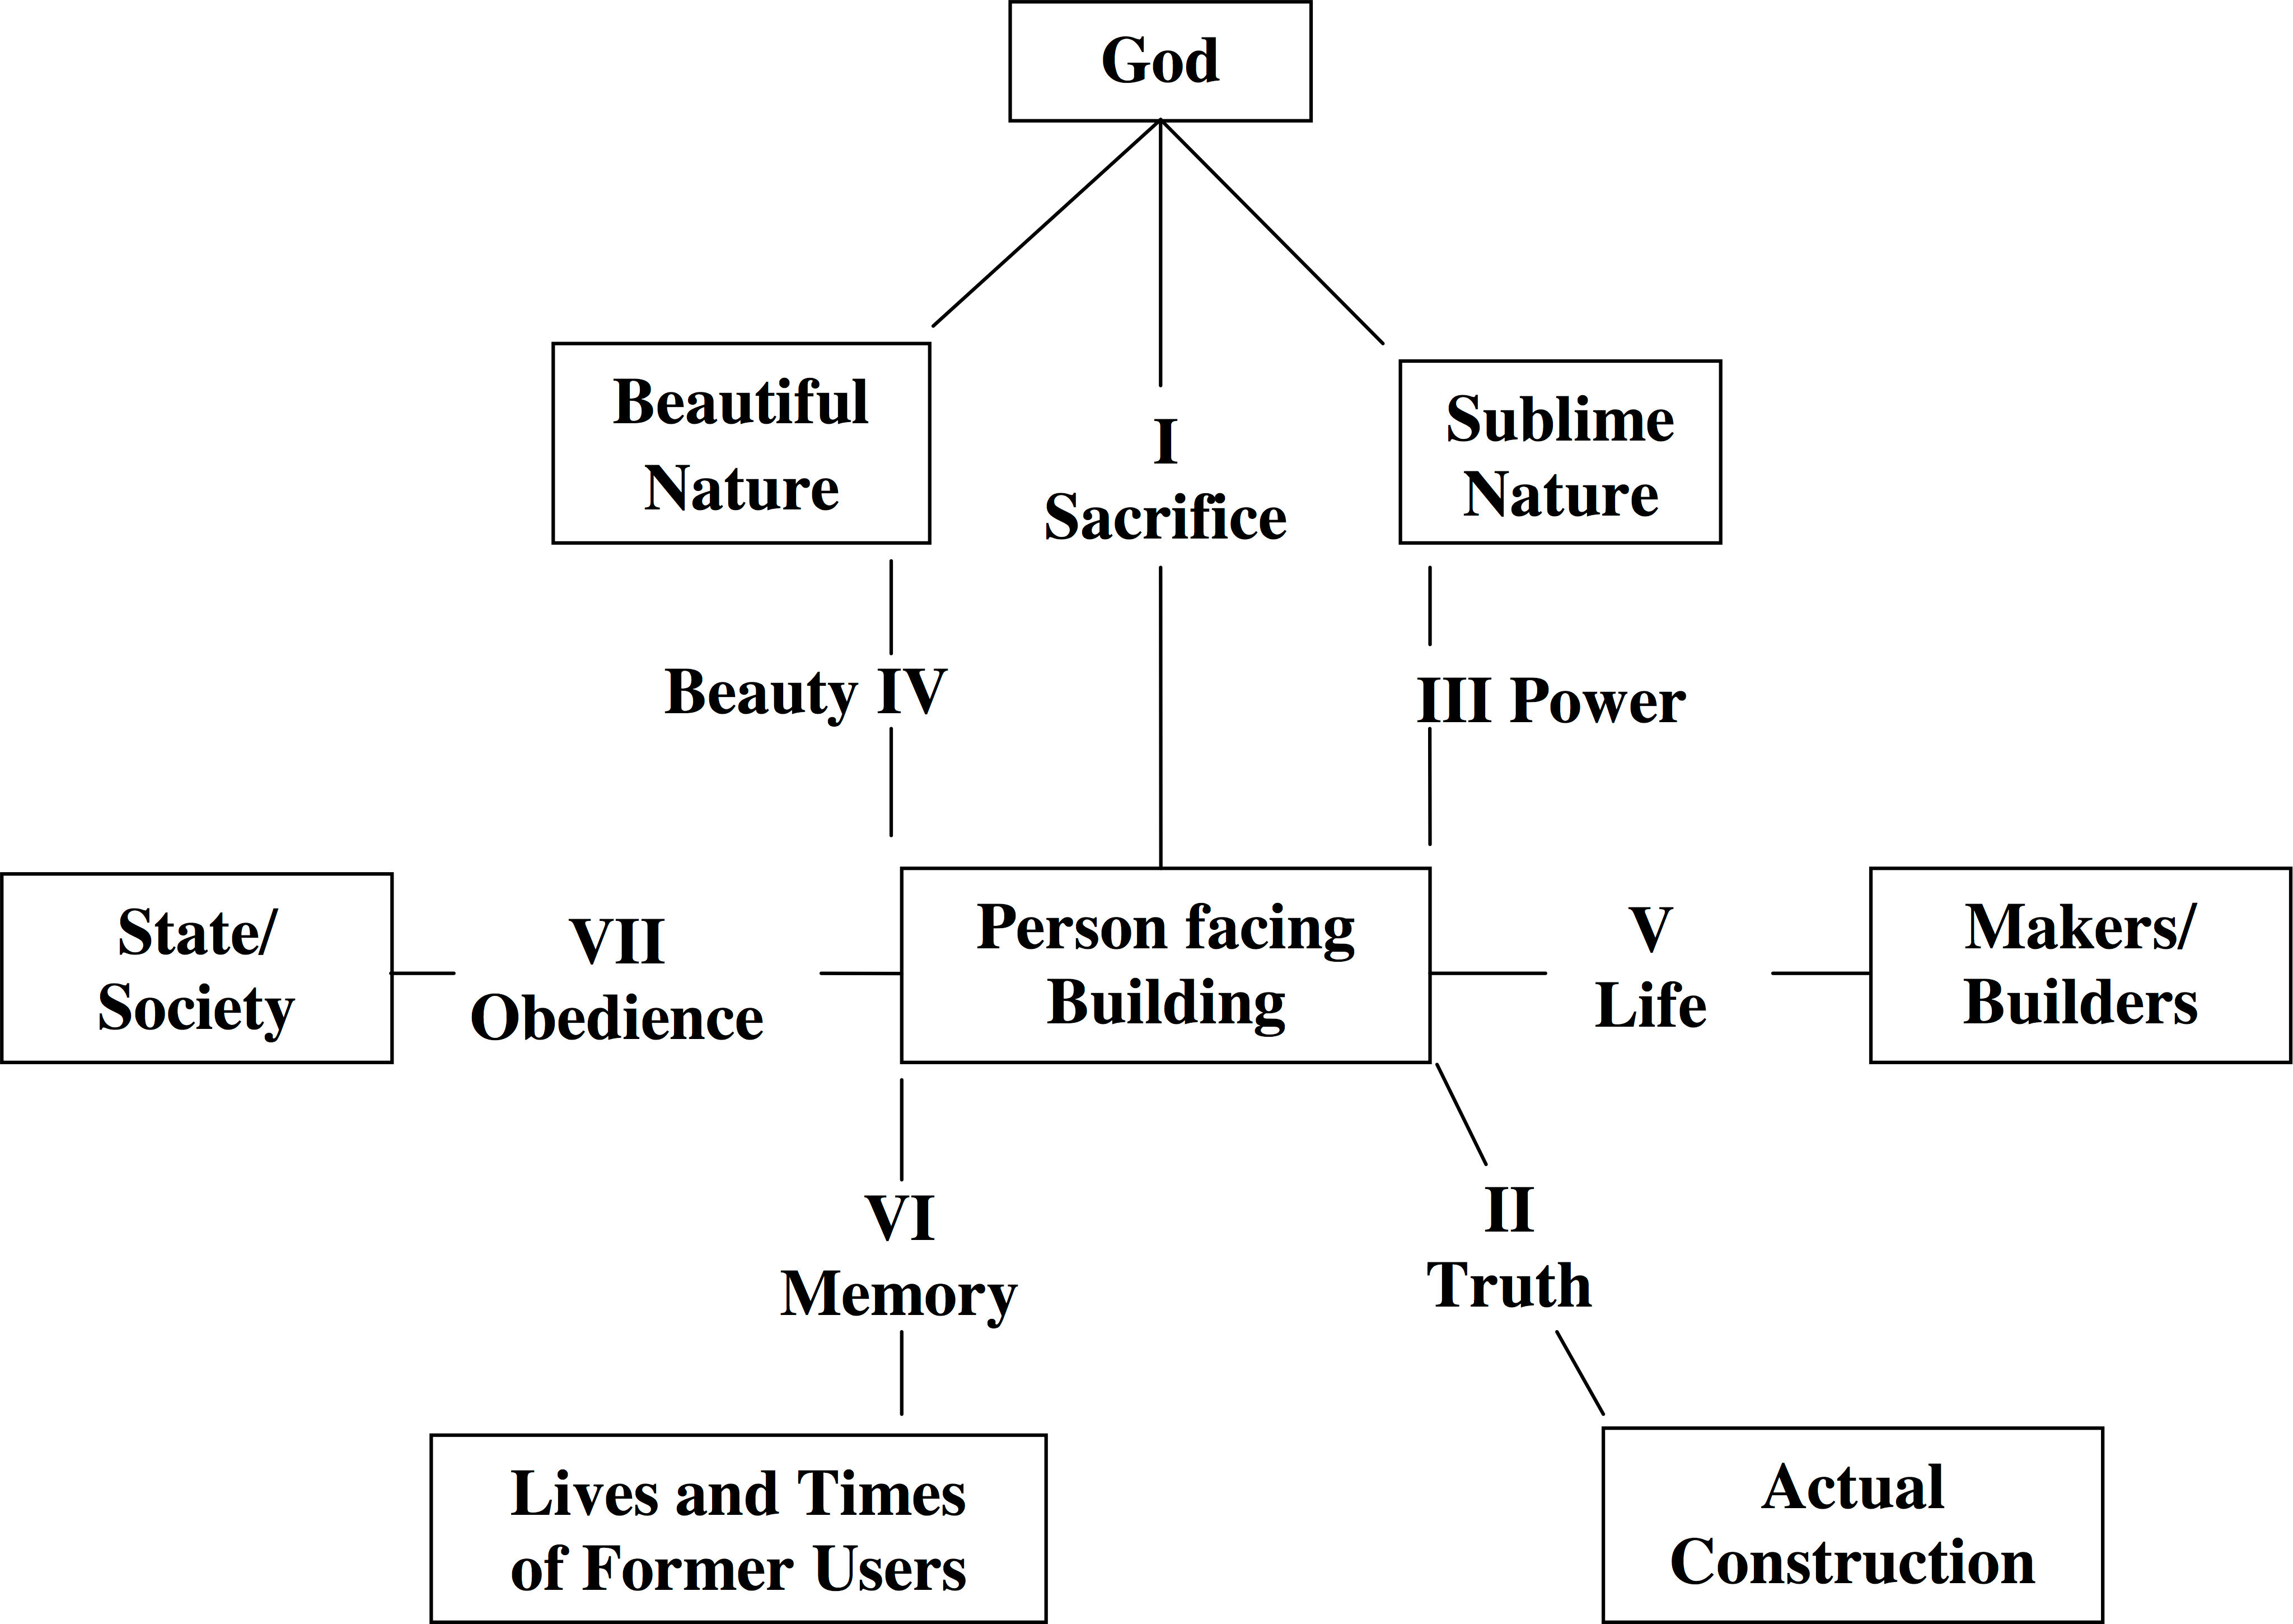
\includegraphics[width=5in]{HallChart.png}
	\caption{Conceptual Scheme of \textit{The Seven Lamps of Architecture}}
	\label{fig:lamps_conceptual}
\end{figure}

Ruskin ties beauty to human beings and their experience with nature in
\textit{The Seven Lamps of Architecture}.  In one diary entry dated
April 19, 1846, Ruskin describes a day in Champagnole, France and then
comments on how nature affected him: 

\index{nature}
\begin{quote}
I felt it more than usual, but it struck me suddenly how utterly
different the impression of such a scene would be, if it were in a
strange land and in one without history.  How dear to the feeling is
the pine of Switzerland compared to that of Canada!  I have allowed too
little weight to these deep sympathies, for I think, if that pine
forest had been among the Alleghanys, or if the stream had been
Niagara, I should only have looked at them with intense melancholy and
desire for home. \citep[][p.~325]{ruskin1956}
\end{quote}

\index{associationism}
\index{beauty}
\index{permanence}
This observation of creation enables Ruskin to embrace the theory of
associationism, especially its connections to history, which influences
his aesthetic appreciation.  George \citet{landow2005} points out that Ruskin’s
emphasis on beauty seems to emerge out of these historical associations
that assist his criticism of contemporary architecture.  Ruskin finds the homes and
public buildings of his England constructed without style, without
regard to permanence and without meaning for the men who inhabit them. 
Since he wishes to correct these deficiencies, he places great emphasis
upon historical associations, whose presence, he says, will insure both
that an edifice influence the life of the inhabitant and that it be
solidly constructed — this latter because if a building is to endure
long enough for historical associations to accrue, then it must be well
made. 

Thus, Ruskin’s establishment of memory as one of his seven laws—with its
focus on the social, historical, and cultural milieu—becomes essential
to his philosophy of architecture. 

\section{Ruskin and \textit{The Stones of Venice}}

\index{St. Mark's Cathedral|(}
\hallfigure{HallImage1.jpg}{St. Mark's Cathedral, by John W. Bunney}{Public Domain}{fig:stmarks}

In \textit{The Stones of Venice,} Ruskin’s vivid description of St.
Mark’s Cathedral (Figure \ref{fig:stmarks}), a most magnificent structure in Venice---“the
most precious building in Europe standing yet in the eyes of men and
the sunshine of heaven”\citep{nyt1880}---and his detailed sketches of the
same (Figures \ref{fig:stmarkssouth}, \ref{fig:stmarksarchivolt}, \ref{fig:stmarksbasket}, \ref{fig:stmarksfacade}, \ref{fig:stmarksnorthwest}, and \ref{fig:stmarkssketch}) demonstrate the ability of the author to pen with
passion and eloquent style, and the artist to draw with precision and
color, the beauty of its architecture: 

\hallfigure{HallImage2.jpg}{The South Side of St. Mark's from the Loggia of the Ducal Palace, Venice, 1851, by John Ruskin}{Public Domain}{fig:stmarkssouth}

\hallfigure{HallImage3.jpg}{Archivolt in St. Mark's, 1853, by John Ruskin}{Public Domain}{fig:stmarksarchivolt}

\hallfigure{HallImage4.jpg}{Basket and Lily Capital, St. Mark's Basilica, Venice, 1849--1852, by John Ruskin}{Public Domain}{fig:stmarksbasket}

\begin{quote}
A multitude of pillars and white domes, clustered into a long low
pyramid of coloured light; a treasure-heap, it seems, partly of gold,
and partly of opal and mother-of-pearl, hollowed beneath into five
great vaulted porches, ceiled with fair mosaic, and beset with
sculpture of alabaster, clear as amber and delicate as ivory —sculpture
fantastic and involved, of palm leaves and lilies, and grapes and
pomegranates, and birds clinging and fluttering among the branches, all
twined together into an endless network of buds and plumes; and, in the
midst of it, the solemn form of angels, sceptred, and robed to the
feet, and leaning to each other across the gates, their figures
indistinct among the gleaming of the golden ground through the leaves
beside them, interrupted and dim, like the morning light as it faded
back among the branches of Eden, when first its gates were
angel-guarded long ago.  And round the walls of the porches there are
set pillars of variegated stones, jasper and porphyry, and deep-green
serpentine spotted with flakes of snow, and marbles, that half refuse
and half yield to the sunshine, Cleopatra-like, ``their
bluest veins to kiss''---the shadow, as it steals back from
them, revealing line after line of azure undulation, as a receding tide
leaves the waved sand; their capitals rich with interwoven tracery,
rooted knots of herbage, and drifting leaves of acanthus and vine, and
mystical signs, all beginning and ending in the Cross; and above them,
in the broad archivolts, a continuous chain of language and of life---angels, 
and the signs of heaven and the labours of men, each in its
appointed season upon the earth; and above these another range of
glittering pinnacles, mixed with white arches edged with scarlet
flowers,—a confusion of delight, amidst which the breasts of the Greek
horses are seen blazing in their breadth of golden strength, and the
St. Mark's Lion, lifted on a blue field covered with
stars, until at last, as if in ecstacy, the crests of the arches break
into a marble foam, and toss themselves far into the blue sky in
flashes and wreaths of sculptured spray, as if the breakers on the Lido
shore had been frost-bound before they fell, and the sea-nymphs had
inlaid them with coral and amethyst.  \citep[][vol. 2, ch. 4, sec. 14]{ruskin1885}
\end{quote}

\hallfigure{HallImage5.jpg}{Northwest Angle of the Fa\c{c}ade, St. Mark's Church, 1851, by John Ruskin}{Public Domain}{fig:stmarksfacade}
\index{St. Mark's Cathedral|)}

\index{beauty}
\index{nature}
These words and drawings reflect the magnificence that resonates in the
actual architecture, authenticating the lamp of beauty, for Ruskin
clearly believes that architecture should reflect the design found in
nature and point towards the ultimate Master Builder.  

\index{aesthetics}
\index{architecture!moral}
\index{architecture!Gothic}
\index{architecture!Renaissance}
With a philosophy based on aesthetics, place, and history, Ruskin
appeals to a moral architecture, encouraging builders to reject the
techniques discovered in the Renaissance and developed in the
Industrial Revolution and to embrace a time when the best buildings
were constructed—the medieval Gothic cathedrals of England and Venice. 
In his later book, \textit{The Stones of Venice }(1851--1853), Ruskin
describes the elements of the Gothic that became foundational for the
kind of architecture he proposes, and he provides many examples to
illustrate.  He points out the three virtues of a building: (1) “That
it act well,” (2) “That it speak well,” and (3) “That it look well” \citep[][vol. 1, ch. 2, sec. 1]{ruskin1885}. 
\index{architecture!virtues}
 
In \textit{The Crown of Wild Olive}, Ruskin
explains the purpose of his writing: 

\hallfigure{HallImage6.jpg}{North West Porch, St. Mark's, Venice, 1877, by John Ruskin}{Public Domain}{fig:stmarksnorthwest}

\index{architecture!Gothic}
\index{architecture!Renaissance}
\begin{quote}
The book I called ``The Seven Lamps'' was to show that certain right
states of temper and moral feeling were the magic powers by which all
good architecture, without exception, had been produced. 
``The Stones of Venice'' had, from beginning to end, no
other aim than to show that the Gothic architecture of Venice had
arisen out of, and indicated in all its features, a state of pure
national faith, and of domestic virtue; and that its Renaissance
architecture had arisen out of, and in all its features indicated, a
state of concealed national infidelity, and of  domestic corruption. 
\citep[][p.~53]{ruskin1866}
\end{quote}

\index{architecture!Gothic}
For Ruskin, moral feeling, states of temperament, and architecture
cannot be separated.  He sees the ``moral elements of Gothic'' as
follows: (1) savageness, (2) changefulness, (3) naturalism, (4)
grotesqueness, (5) rigidity, and (6) redundance, when “belonging to the
building,” and (1) savageness or rudeness, (2) love of change, (3) love
of nature, (4) disturbed imagination, (5) obstinancy, and (6)
generosity, when “belonging to the builder” \citep[][p.~155]{ruskin1885}.
Thus, Ruskin was not arguing for a new style of architecture. 
He was lamenting the plainness and the soullessness of the architecture
designed and built since the Gothic cathedrals of the medieval period. 
He “found certain
styles (e.g., Baroque) unacceptable because they exploited illusions,
and therefore were not `truthful'”\citep[][p.~669]{curl2006}.
Therefore, according to Ruskin, in order for architecture
to be sincerely honest and truly beautiful, it must be connected to
nature, rooted in right history, and constructed by human hands.  
\index{truth}

\section{Review of Ruskin's Reputation}

\hallfigure{HallImage7.jpg}{Part of St. Mark's, Venice, Sketch After Rain, 1846, by John Ruskin}{Public Domain}{fig:stmarkssketch}

\index{architecture!role}
\index{Kerr, Robert}
The appeal of Ruskin’s philosophy of architecture was paramount during
the Victorian period.  Professor Robert Kerr, a contemporary of the art
critic, had previously espoused the same ideas as Ruskin, but he had
left them behind after working twenty years in the field.  He
encouraged experienced architects to deter younger apprentices from the
idealistic and romanticized views of Ruskin, for Kerr viewed the
architect as “a servant of the public for the efficient design of
buildings, precisely like the engineer.”  When he presented a lecture
entitled ``Architectural Criticism'' at the
Royal Institute of British Architects, he severely criticized Ruskin
saying that “Mr. Ruskin's thoughts soar high enough in
the poetry of visionary art, because poetry is his business, but they
cannot stoop down to the plain prosaic details of the structuresque,
because building is not his business” \citep[][pp.~259--260]{collins1998}.  In an
October 1849 review of \textit{The Seven Lamps of Architecture
}published in the \textit{Journal of Design}, Matthew Digby Wyatt
admired “the excellent spirit” that was present in “this thoughtful,
eloquent book.”  However, he quickly points out that Ruskin “either
puts his back against  [. . .] further development, or would attempt to
bring back the world of art to what its course of actions was four
centuries ago!” \citep[][pp.~121,~438]{mallgrave2009}

\index{St. Mark's Cathedral|(}
Ruskin does not hesitate to move from art critic to social critic,
demonstrating how the architecture itself can become a commentary on
the denigration, deterioration, and degradation of society.  Even as he
praises the majesty of St. Mark's in \textit{The
Stones of Venice}, he also notes the ironic contrast that takes place
in its shadows as the masses ignore its beauty and the poor grovel in
their poverty.  

\begin{quote}
And what effect has this splendor on those who pass beneath it?  You may
walk from sunrise to sunset, to and fro, before the gateway of St.
Mark’s, and you will not see an eye lifted to it, nor a countenance
brightened by it.  Priest and layman, soldier and civilian, rich and
poor, pass by it alike regardlessly.  Up to the very recesses of the
porches, the meanest tradesmen of the city push their counters; nay,
the foundations of its pillars are themselves the seats—not “of them
that sell doves” for sacrifice, but of the vendors of toys and
caricatures.  Round the whole square in front of the church there is
almost a continuous line of cafés, where the idle Venetians of the
middle classes lounge, and read empty journals; in its centre the
Austrian bands play during the time of vespers, their martial music
jarring with the organ~notes,—the march drowning the miserere, and the
sullen crowd thickening round them,—a crowd, which, if it had its will,
would stiletto every soldier that pipes to it.  And in the recesses of
the porches, all day long, knots of men of the lowest classes,
unemployed and listless, lie basking in the sun like lizards; and
unregarded children,—every heavy glance of their young eyes full of
desperation and stony depravity, and their throats hoarse with
cursing,—gamble, and fight, and snarl, and sleep, hour after hour,
clashing their bruised centesimi upon the marble ledges of the church
porch.  And the images of Christ and His angels look down upon it
continually. \citep[][vol. 2, ch. 4, sec. 15]{ruskin1885}
\end{quote}

Ruskin observes that society and architecture are invariably connected.

John Matteson makes this observation concerning Ruskin the social
critic: ``The architecture was sublime; the human activity
around it was an obscene mockery.  What good was the building if it
could not transform the debauched children who cast lots on its very
steps?  After \textit{The Stones of Venice}, it was no longer enough
for Ruskin to criticize art.  It was hierarchies of human beings, not
structures of wood and stone, that begged most loudly for his
attention''\citep[][p.~302]{matteson2002}.
\index{St. Mark's Cathedral|)}

\section[Ruskin's Relevance]{Ruskin's Relevance to Contemporary Architecture}

\hallfigure{HallImage8.jpg}{Crystal Palace, Sydenham, by Achille-Louis Martinet}{Public Domain}{fig:crystalpalace}

Clearly then Ruskin spoke to the Victorian period, but the question
inescapably arises, Can the aesthetic and moral philosophies of a
Victorian art and social critic be applicable to design and
construction today?  Is Ruskin relevant to contemporary architecture? 

\index{Crystal Palace}
\hallfigure{HallImage9.jpg}{Queen Victoria Opening the 1862 Exhibition (inside view of Crystal Palace), by Joseph Nash}{Public Domain}{fig:qvopening}

John Matteson discusses this very question.  Citing the building of the
Crystal Palace (Figures \ref{fig:crystalpalace} and \ref{fig:qvopening}), 
whose ``prefabricated components heralded a
revolution,'' which was occurring at the same time as the publication of
Ruskin's \textit{Stones of Venice}, Matteson asserts
that ``Ruskin’s ideas were already destined for quaintness in the
1850s'' \citep[][p.~300]{matteson2002}.  He points out some of the difficulties of
applying Ruskin's first principles to contemporary
architecture: 

\hallfigure{HallImage10.jpg}{Cathedral of St. John the Divine, Wide Angle View}{Copyright \textcopyright\ 2011 Kirpaks and licensed for reuse under the Creative Commons Attribution-ShareAlike License}{fig:stjohnwide}

\begin{quote}
Since Ruskin’s time, populations have grown and economic systems have
expanded with once unimaginable speed.  Construction in our time has to
be fast.  It must be efficient.  It must avoid unnecessary expense.  If
Ruskin foresaw the further mechanization of physical labor, he was at
least spared the sadness of seeing how far that mechanization would
eventually extend.  Ruskin also did not anticipate that the alienation
that he saw as poisoning the life of the worker might someday encompass
not only the process of construction, but also those of conception and
design.  He could never have imagined on-line catalogs of design
components or the idea that an architect might one day resolve
decisions of ornamentation, not with painstaking manual drawing or
model-building, but with the click of a mouse.  Neither could he have
expected that modern buildings would often be commissioned and
designed, not by individuals at all, but by impersonal organizations. 
It would have been strange, indeed, for Ruskin to discover the myriad
ways in which architecture could divorce itself from the simple human
acts of drawing and carving. \citep[][p.~300]{matteson2002}
\end{quote}

\index{Cathedral of St. John the Divine|(}
Yet Matteson does not completely reject Ruskin’s writings about Gothic
architecture, citing the construction of St. John the Divine in
Manhattan (Figures \ref{fig:stjohnwide} and \ref{fig:stjohnwestern}) as an exemplar of Ruskinian ideals.  In 1972,
after no construction had occurred on the building for thirty years,
the dean of St. John the Divine proclaimed that it was time to once
again begin work and that “the stonework [would] be done by our own
unemployed and underemployed neighbors.  We will revive the art of
stonecraft”\citep[][p.~300]{matteson2002}. Matteson observes that both the
process and the product were ``profoundly
Ruskinian'': 

\hallfigure{HallImage11.jpg}{Cathedral of St. John the Divine, The Western fa\c{c}ade, including the Rose Window}{Copyright \textcopyright\ 2008 William Porto and licensed for reuse under the Creative Commons Attribution-ShareAlike License}{fig:stjohnwestern}

\begin{quote}
The spirit of the new construction was profoundly Ruskinian: it
entrusted a sacred Gothic edifice to hands that would begin the project
raw and untutored, in expectation that, as the structure grew and took
shape, so, too, would the skills and souls of the workers.  That the
cathedral actually did become a literal synthesis of stonecutting and
soul-making, an exemplar of Ruskin’s demand that the work must affirm
the passion of the worker, seems to be confirmed in the words of Simon
Verity, one of the master carvers employed in the project: “To be a
carver, you have to have a passion for it, to love it with all your
heart.  It’s a desire to create order out of chaos, to seek 
harmonies.” \citep[][pp.~300--301]{matteson2002}
\end{quote}

For Matteson, unskilled human hands touching and carving stone so that
both are built together reflect the perfect aesthetic and moral for the
Ruskinian model, celebrating Ruskin’s laws of life and truth.  He
concludes, “Surely, Ruskin would have applauded this method of
construction, a combination, someone has said, of outreach and
up-reach.  And yet his applause might have been tempered by the
knowledge of how deeply the impersonality of technology and profit had
insinuated themselves into the building of the cathedral” \citep[][p.~301]{matteson2002}.  
\index{Cathedral of St. John the Divine|)}

\section{Architecture as a Palimpsest}

\hallfigure{HallImage12.jpg}{A Georgian palimpsest of the 5th/6th century}{Public Domain}{fig:georgianpalimpsest}

\index{Carlyle, Thomas}
\index{palimpsest|see{architecture, as palimpsest}}
\index{architecture!as palimpsest|(}
\index{social memory}
During the Victorian era, Thomas Carlyle (1830), like Ruskin, also
demanded that attention be given to history.  In his essay “On History”
(1830), he says that meaning in the present and the future can be known
only as the past is studied.  He writes: ``For though the
whole meaning lies far beyond our ken; yet in that complex Manuscript
covered over with formless inextricably-entangled unknown
characters,---nay which is a \textit{Palimpsest}, and had once
prophetic writing, still dimly legible there,---some letters, some
words, may be deciphered'' (author's emphasis) \citep[][p.~56]{carlyle1971}.  
Uhlig
concurs with Carlyle and maintains that in the intertext, which he
likens to the palimpsest (Figures \ref{fig:georgianpalimpsest}, \ref{fig:archimedes1}, and \ref{fig:archimedes2}), “historically conditioned
tensions come to the fore: tensions not only between calendar time and
intraliterary time but also between the author’s intention and the
relative autonomy of a text, or between the old and the new in general”
\citep[][p.~502]{uhlig1985}.  The presence of the past coexists with the text; thus,
``any text will the more inevitably take on the
characteristics of a palimpsest the more openly it allows the voices of
the dead to speak, thus---in a literary transcription of our cultural
heritage---bringing about a consciousness of the presentness of the
past'' \citep[][p.~502]{uhlig1985}.  Deciphering the present moment of the
text as it relates to many past moments reveals the intertextual
meaning the text seeks to convey and the critic to uncover. 

\index{Archimedes Palimpsest}
\hallfigure{HallImage13.jpg}{Archimedes Palimpsest}{Copyright \textcopyright\ Rochester Institute of Technology, Equipoise Imaging and Boeing LTS and licensed for reuse under the Creative Commons Attribution-ShareAlike License}{fig:archimedes1}
\index{palimpsests!examples|(}
The word ``palimpsest'' derives from
$\pi \alpha \lambda \text{\textgreek{'i}}\mu \psi \eta \sigma \tau
o\varsigma $ (\textit{palimpsestos}) which is Greek in origin and means
``scraped again'' \citep{liddellscott1990} %% FIXME - this said 1929
and can be defined as ``a papyrus or other kind of writing
material on which two or more sets of writing had been superimposed in
such a way that, because of imperfect erasure, some of the earlier text
could be read through over-writing''\citep[][p.~309]{darville2002}.  When
used in the field of archaeology, ``the term is often
applied to landscapes in which traces of earlier arrangements can be
seen amongst and below the modern pattern''\citep[][p.~309]{darville2002}, 
and in architecture palimpsest means the shadow of a past
structure that is in some way incorporated as part of an old one that
has been remodeled or a new one that has been built.  Michael Earle
describes the concept as follows: 

\hallfigure{HallImage14.jpg}{Archimedes Palimpsest}{Copyright \textcopyright\ Rochester Institute of Technology, Equipoise Imaging and Boeing LTS and licensed for reuse under the Creative Commons Attribution-ShareAlike}{fig:archimedes2}

\begin{quote}
Architects use the concept of palimpsest to imply a ghost, an image of
what once was.  Of course, in the built environment, this occurs often,
whenever spaces are shuffled, rebuilt, or remodeled, shadows remain. 
Tarred rooflines remain on the sides of a building long after the
neighboring structure has been demolished and long ago removed stairs
leave a mark where the painted wall surface stopped.  Dust lines remain
from a relocated appliance.  Ancient ruins speak volumes of their
former wholeness.  Palimpsests can inform us of the realities of the
built past. \citep{earle2012}
\end{quote}
\index{palimpsests!examples|)}

\index{dynamism}
\index{stasis}
According to Peter Eisenman, an architect and theorist, the palimpsestic
connection of site history with contemporary design and construction is
essential: ``Any site contains not only presences, but the memory of
previous presences and the immanences of a possible presence.  The
physical difference between a moving thing (dynamism) and a still one
(stasis) is that the moving one contains the trace of where it has been
and where it is going.''  He then connects the history to
the city itself, seeing it as an integral part of the site: “The
introduction of this trace, or condition of absence, acknowledges the
dynamic reality of the living city” \citep[][p.~207]{eisenman2004}.  Eisenman describes an architectural
palimpsestic text as follows: 

\index{architecture!as text|(}
\begin{quote}
In my proposal for rhetorical figures, architecture is no longer
elements but an \textit{other} grammatical counter, proposing an
alternate reading of the idea of site and object.  ~In this sense, a
rhetorical figure will be seen to be inherently contextual in that the
site is treated as a deeply scored palimpsest. [. . .] This text
suggests that there are other meanings which are site specific by
virtue of their pre-existence, however latent within the context. 
\citep[][p.~206]{eisenman2004}
\end{quote}

He explains that the word ``text'' when used
in relationship to architecture 

\begin{quote}
can be used for any and all strategies and conditions which dislocate
architecture from its authorial or natural condition of being; that is,
the detaching of what architecture looks like from the need to
represent function, shelter, meaning and so forth.  It is not so much
that the look of architecture will change (architecture will always
look like architecture) but rather the style and significance of its
look will be different.  The idea of text is not in opposition to the
reality of architecture, just as the imaginary is not the opposite of
the real; it is an \textit{other} discourse.  Text surrounds reality at
the same time that it is internal to reality. \citep{eisenman1988}
\end{quote}

Eisenman, like Ruskin, sees that architecture communicates a text beyond
its outward beauty: ``Thus in architecture it is possible
to say that text is what always exceeds the immediate response to a
visual or sensory image, i.e. that which we see on the surface as the
story, or that which we see as the beautiful.  This is the heart of the
matter''\citep{eisenman1988}.  Thus, a palimpsest can
be defined as that text which underlies another text (an ur-text)---a
present text with origins in a past one (palingenesis) or at least
shaped by an underlying one (ananke)---or a text that influences
something not of its own genre---art, music, architecture \citep[][p.~503]{uhlig1985}. 
\index{architecture!as palimpsest|)}
\index{architecture!as text|)}

\section[Peter Eisenman and \textit{The Memorial}]{Peter Eisenman and \textit{The Memorial for the Murdered Jews of Europe}}

\index{Memorial to the Murdered Jews of Europe|(}
\hallfigure{HallImage15.jpg}{Memorial to the Murdered Jews of Europe, Peter Eisenman}{Public Domain}{fig:memorial1}
Finished in 2004 and inaugurated on May 10, 2005---sixty years after
the conclusion of World War II---The Memorial to the Murdered Jews of
Europe (Figures \ref{fig:memorial1} and \ref{fig:memorial2}), also known as the Holocaust Memorial, was built
in Berlin by Peter Eisenman, an American architect \citep{brunberg2012}. 
Encompassing five and a half acres \citep{ouroussoff2005}, it is designed with
“2,711 pillars, planted close together in undulating waves,
represent[ing] the 6 million murdered Jews” \citep{quigley2005}.  The memorial is
open every day year round and can be entered on each of the four sides
\citep{quigley2005}.  

True to his architectural theory, Eisenman is focused on
incorporating the memorial into its site and to the city itself
\citep{quigley2005}, “acknowledge[ing] the dynamic reality of the living city” \citep[][p.~207]{eisenman2004}

Nicolai Ouroussoff explains: 

\hallfigure{HallImage16.jpg}{Memorial to the Murdered Jews of Europe, Peter Eisenman}{Copyright \textcopyright\ 2005 de:Benutzer:Schreibkraft and licensed for reuse under the Creative Commons Attribution-ShareAlike License}{fig:memorial2}

\begin{quote}
At first, you retain glimpses of the city.  The rows
of pillars frame a distant view of the Reichstag's
skeletal glass dome.  To the west, you can glimpse the canopy of trees
in the Tiergarten.  Then as you descend further, the views begin to
disappear.  The sound of gravel crunching under your feet gets more
perceptible; the gray pillars, their towering forms tilting unsteadily,
become more menacing and oppressive.  The effect is intentionally
disorienting. \citep{ouroussoff2005}
\end{quote}

The construction arises out of the city’s history,
bringing it into the present: “The memorial's grid,
for example, can be read as both an extension of the streets that
surround the site and an unnerving evocation of the rigid discipline
and bureaucratic order that kept the killing machine grinding along. 
The pillars, meanwhile, are an obvious reference to tombstones” \citep{ouroussoff2005}.  
Yet observation alone is not enough; one must
experience the site “as a physical space” in order to truly understand
it: 

\begin{quote}
No clear line, for example, divides the site from the
city around it.  The pillars along its periphery are roughly the height
of park benches.  A few scattered linden trees sprout between the
pillars along the memorial's western edge; at other
points, outlines of pillars are etched onto the sidewalk, so that
pedestrians can actually step on them as they walk by. \citep{ouroussoff2005}
\end{quote}

Sarah Quigley, a novelist and critic, describes her encounter with the
memorial: 

\begin{quote}
Even on bright sunny days, the
stones look sober and drab.  Standing on an uneven piece of land, the
stelae almost fall into the centre of the site, rising up again towards
the edge, forming a myriad of uneven stone corridors.  Walking down one
of these passages is disorientating, and scary; you can’t see who is
approaching you, nor who is behind.  The tilting ground and lack of
vision offers some small idea of the Jewish experience from WWII: your
past snatched away, your future insecure, little hope of escape. \citep{quigley2005}
\end{quote}

In this memorial the past haunts both the present and the future.

Somewhat unexpectedly, Eisenman rediscovered his Jewishness in this
architecture: “[With this work] I came back to the heart of my
identity” \citep{quigley2005}.  Even so, Eisenman is not interested in
viewing the Holocaust with sentimentality.  He does not
``want people to weep and then walk
away with a clear conscience'' \citep{ouroussoff2005}.  He
wants all who visit to realize their culpability, to understand ``the
process that allows human beings to accept such evil as part of the
normal world - the incremental decisions that collectively lead to the
most murderous acts'' \citep{ouroussoff2005}. Eisenman “leaves you standing on the edge of the
abyss.  In so doing, he suggests that the parameters of guilt are not
so easily defined: it includes those who looked the other way,
continued with their work, refused to bear witness.  It is true of
Americans as well as Germans, Roman Catholic clerics as well as Nazi
secretaries” \citep{ouroussoff2005}. 

In contrast to Ruskin who believed that architecture should reflect
beauty and point upward to the ultimate Maker, Eisenman’s design is
plain and its purpose is to cause the viewer to look inward.  Although
Paul Spiegel, a leader of the Jews in Germany, felt that the memorial
was “incomplete” because it did not shock those who saw it with its
history, Eisenman’s desire was to promote and elicit a response that
concerned more than just the Holocaust; he wanted people to focus on
anti-Semitism in general and civilization’s response to it.  This
discussion would broaden the appeal of the memorial and make it a part
of the daily life of the city \citep{quigley2005}.  Perhaps this statement
encapsulates Eisenman’s attitude most of all:
“I think people will eat their lunch on
the pillars. [. . .] I’m sure skateboarders will use it.  People will
dance on top of the pillars.  All kinds of unexpected things are going
to happen” \citep{quigley2005}.  Eisenman’s prediction has already come
true, for Nicolai Ouroussoff writes, “The day I visited the
site, a 2-year-old boy was playing atop the pillars - trying to climb
from one to the next as his mother calmly gripped his hand” \citep{ouroussoff2005}.

The palimpsest of the Holocaust surrounds the site.  Nicolai
Ouroussoff asserts, “The location could not be more
apt.  During the war, this was the administrative locus of
Hitler's killing machine.  His chancellery building,
designed by Albert Speer and since demolished, was a
few hundred yards away just to the south; his bunker lies beneath a
nearby parking lot.” \citep{ouroussoff2005}  Although criticized by some well-known Germans
for its abstract symbolism, its dreary atmosphere, and its sparse
construction \citep{quigley2005} (e.g., no names are etched into the pillars
[\citealp{brunberg2012}]), Eisenman insists that The Memorial for the Murdered Jews
of Europe “is both perfect in its symbolism, and a necessary aid to
atonement.  ‘It stands there, silent,’ he says: ‘the one who has to
talk is you’” \citep{quigley2005}.
\index{Memorial to the Murdered Jews of Europe|)}

\section{Daniel Libeskind and His Architecture}

\index{Libeskind, Daniel|(}
\subsection{\textit{The Jewish Museum Berlin}}

\index{The Jewish Museum Berlin|(}
\hallfigure{HallImage17.jpg}{The Jewish Museum Berlin, to the left of the old Kollegienhaus.  Designed by Daniel Libeskind}{Copyright \textcopyright\ 2008 Daniel Libeskind and licensed for reuse under the Creative Commons Attribution-ShareAlike License}{fig:jewishmuseum}

Opened in 2001, The Jewish Museum Berlin (Figure \ref{fig:jewishmuseum}) showcases 1700
years of the history of the Jews in Germany.  Two buildings house the
exhibits, the old \textit{Kollegienhaus}, once used as a courthouse,
and a new one designed by Daniel Libeskind.  The museum covers 166,840
square feet \citep{libeskind2011} and is constructed as a twisted zig-zag
to remind museum-goers of a warped Star of David \citep{muellerkroll2011}.  It
is entered through an underground tunnel.  A
``Void''---a space with nothing in it except
10,000 iron faces that are called ``Fallen Leaves,'' created by
an artist from Israel,
Menashe Kadishman---is part of the memorial \citep{berlin2012}.
One visitor describes his experience in this manner:

\begin{quote}
On the floor, thousands of pieces of heavy metal cut
into shapes of the faces of screaming holocaust victims.  The visitor
is encouraged to walk across the void.  Clank, clank, clank echoing up
into and all around the void.  The noise rings in your head but there
is no escape because as you are tempted to look down the screaming
faces stare into your psyche.  Very simple, very effective.  Haunting. \citep{gold2004}
\end{quote}

The memorial has three intersecting tunnels that are said to represent
three pathways of German life for the Jew: the Axis of Continuity (with
German history), the Axis of Emigration (from
Germany), and the Axis of the Holocaust.  Then the participant moves
into the Garden of Exile with its 49 pillars that reminds visitors of
the people expelled from Germany, which according to Libeskind, is
designed ``to completely disorient the visitor.  It
represents a shipwreck of history.''  Even so, Russian
willow oak trees that represent hope have been planted on top of the
stelae \citep{berlin2012c}.

Libeskind’s design entitled “Between the Lines” was chosen from a
world-wide competition of 165 entries \citep{levenson2005}, and, of course, the
architect was ecstatic when he won: “It was a thrilling moment when I
was selected.  The jury recognized that my plan was neither dogmatic
nor glib; that it served as an individualized mirror, which each
visitor could read in a different way.  They valued its authenticity
and celebrated its originality. I felt honored and elated” \citep[][p.~85]{libeskind2004}.

Because of his own personal background and experience, Daniel Libeskind
knew that the architecture must first connect the place to its history
and then take visitors from the past to the present and propel them to
the future, experiencing a sense of alienation: 

\begin{quote}
You struggle to find the most immediate way to get at the truth.  What
was needed, as I saw it, was a building that, using the language of
architecture, speaking from its stones, could take us all, Jews and
non-Jews alike, to the crossroads of history, and show us that when the
Jews were exiled from Berlin, at that moment, Berlin was exiled from
its past, its present, and—until this tragic relationship is resolved—
its future.  \citep[][p.~83]{libeskind2004}
\end{quote}

At this museum, Daniel
Libeskind believes history and architecture are joined, for this place
``thematizes and integrates, for the first time in
post-war Germany, the history of the Jews in Germany, the repercussions
of the Holocaust and spiritual displacement.  It is also just a museum
with exhibits on the wall'' \citep{muellerkroll2011}.
\index{The Jewish Museum Berlin|)}

\subsection{\textit{The One World Trade Center}}

\index{The One World Trade Center|(}
\hallfigure{HallImage18.jpg}{Ground Zero Master Plan (2006)}{Copyright \textcopyright\ Silverstein Properties}{fig:groundzeroplan}

Winning the design competition in 2003 out of more than 10,000
entrants with his Memory Foundations plan (titled this, per Libeskind, “because it’s
about memory and at the center of it is a foundation for
21\textsuperscript{st} century New York” [\citealp{nessen2011}])—originally known as the Gardens of the World \citep{hirschkorn2003, swanson2011, ny1news2003}, Daniel Libeskind was chosen as the
architect to create the Ground Zero Master Plan for the reconstruction
of the World Trade Center (Figure \ref{fig:groundzeroplan}) \citep{libeskind2011}.  As he put
together the design, he realized, ``We have to be able to
enter this hallowed, sacred ground while creating a quiet, meditative
and spiritual space''\citep{libeskind2012}.  He was very
sensitive to the site and to New Yorkers, desiring for his plan to
fully memorialize what had happened there: 

\begin{quote}
When I first began this project, New Yorkers were divided as to whether
to keep the site of the World Trade Center empty or to fill the site
completely and build upon it.  I meditated many days on this seemingly
impossible dichotomy.  To acknowledge the terrible deaths which
occurred on this site, while looking to the future with hope, seemed
like two moments which could not be joined.  I sought to find a
solution which would bring these seemingly contradictory viewpoints
into an unexpected unity.  So, I went to look at the site, to stand
within it, to see people walking around it, to feel its power and to
listen to its voices. \citep{libeskind2012}
\end{quote}

For Libeskind, this project was personal: “What happened on 9/11 was
not something abstract, it happened to me” (qtd. in
Earle). In fact, on the day Libenskind opened his
Jewish Museum in Berlin, the Twin Towers in New York were attacked and
then collapsed.  As soon as he received word around 2:30 p.m., he left
for the States.  He still  remembers that day, ``I turned
to all my colleagues [. . .] and I do not know where it came from, but
I said, `I'm returning to Lower
Manhattan{'}'' \citep{huffpost2012}.
%% FIXME - quote within a quote - should I switch to textit?

Because of disagreements among all those involved, the project was
eventually removed from Libenskind \citep{huffpost2012}.  Even though
many architectural changes were made, the WTC Masterplan (Figure \ref{fig:groundzeroplan}) as
delineated by Libeskind was still basically followed: 

\begin{quote}
``The WTC Masterplan serves as both the conceptual
basis and the technical foundation for the entire complex
re-development of ground zero.  The Masterplan defines the spirit of
the approach to re-building and creates a meaningful conceptual
framework for the site.  It also defines the spatial organization of
all elements of the development within the site with an emphasis on the
human experience and the public realm.  The Masterplan dictates the
location and massing of each program element, building height and
relative size, as well as proximity and relationship to one another. 
The WTC Masterplan also supplies the framework for the site’s
infrastructure, transportation, sustainability standards and security
strategy and lays out the functional relationship between all the site
elements with respect to the surrounding context of the immediate
neighbourhoods and the surrounding city.'' \citep{libeskind2011}
\end{quote}

Michael Arad, the final designer, credits Libeskind as
the one who “‘established the broad parameters’ of what is now the new
World Trade Center and ‘acted as a guidestar.  If
you're going to build something,
you need to start some place.’”  Libeskind acknowledges his part in the
process: ``I'm so happy to be able to
design a piece of this city.''  He observes,
``If you're a conductor or a composer,
Stravinsky or Copland, and the New York Philharmonic is performing your
piece and you're conducting it, do you regret that
you're not playing the first violin?  That
you're not playing the tuba?  Of course not'' \citep{huffpost2012}.
Therefore, he
asserts confidently, “In the end, the public will see the symbolism of
the site.  [. . .] Of course, compromises had to be made, but a master
plan is not about a few lines drawn on paper.  It’s about an idea, and
how to express that idea through the turmoil of politics and the
creativity of all the other architects.  In the end, the result will be
pretty close to my original rendering” \citep{davidson2007}.

\index{architecture!symbolism|(}
Libenskind’s
original plan reflects his intense interest in symbolism.  He wanted
the foundations of the former buildings to be part of the memorial site
(“We need to journey down, some 70 feet into Ground Zero, onto the
bedrock foundation, a procession with deliberation into the deep
indelible footprints of Tower One and Tower Two”),
and he emphasized
their connection to the nation itself. 

\begin{quote}
The great slurry walls are the most dramatic elements which survived the
attack, an engineering wonder constructed on bedrock foundations and
designed to hold back the Hudson River.  The foundations withstood the
unimaginable trauma of the destruction and stand as eloquent as the
Constitution itself asserting the durability of Democracy and the value
of individual life. \citep{libeskind2012}
\end{quote}

Libeskind imagined “the sky” as “home again” to “vertical gardens” on “a
towering spire of 1776 feet high” (symbolic of the founding of the
country, the year when the Declaration of Independence was signed)—the
“Gardens of the World,” filled with plants from all parts of the earth
 \citep{libeskind2012, ny1news2003, nessen2011}.
He explains, “Why gardens?  Because gardens are a constant affirmation of
life.  A skyscraper rises above its predecessors, reasserting the
pre-eminence of freedom and beauty, restoring the spiritual peak to the
city, creating an icon that speaks of our vitality in the face of
danger and our optimism in the aftermath of tragedy” \citep{libeskind2012}.
\index{architecture!symbolism|)}

\index{Statue of Liberty}
Reminiscent of the
Statue of Liberty, the tower would be off-center in its northwest
corner, designed to pay homage to the Statue of Liberty’s torch which
Libeskind remembers seeing when he was 13 years old in 1959 when he
came to the United States from Poland \citep{swanson2011}.  Indeed Libeskind’s
ideas emerge out of his experience as an immigrant.  He explains in his
proposal for the reconstruction of Ground Zero: ``I
arrived by ship to New York as a teenager, an immigrant, and like
millions of others before me, my first sight was the Statue of Liberty
and the amazing skyline of Manhattan.  I have never forgotten that
sight or what it stands for.  This is what this project is all about'' \citep{libeskind2012}.

\index{Wedge of Light}
\index{Park of Heroes}
The Wedge of Light piazza and the Park of Heroes open spaces were
significant places in Daniel Libeskind's plan
\citep{manhattan2003}.  Libeskind explains how his design
remembers the ones who died: “Those who were lost
have become heroes.  To commemorate those lost lives, I created two
large public places, the Park of Heroes and the Wedge of Light.  Each
year on September 11th between the hours of 8:46 a.m., when the first
airplane hit and 10:28 a.m., when the second tower collapsed, the sun
will shine without shadow, in perpetual tribute to altruism and
courage” \citep{libeskind2012}.  Once again, the symbolism
is paramount.  

\hallfigure{HallImage19.jpg}{One World Trade Center design released in May 2012}{Public Domain}{fig:oneworld}

\index{social history}
The construction of the lynchpin building finally started in 2006
and is scheduled to be finished in 2014.  The One World Trade Center,
or the 1 WTC, previously called the Freedom Tower (Figure \ref{fig:oneworld}), will
occupy the place where the original 6 World Trade Center stood.  When
completed, the 1 WTC will be the tallest building in the Western
Hemisphere rising 1,776 feet as originally envisioned by Libeskind \citep{habitat2012}.  Like Ruskin and Eisenman, Libeskind’s design is
inextricably linked to history.  As Michael Earle observes, ``In terms
of design, his best buildings are connected strongly to history and are
deeply influenced by it.''  His masterplan is ``a palimpsest of the site
itself''\citep{earle2012}.  The past coexists with the architectural texts, and
thus reaffirms that ``any text will the more inevitably take on the
characteristics of a palimpsest the more openly it allows the voices of
the dead to speak, thus [. . .] bringing about a consciousness of the
presentness of the past'' \citep[][p.~502]{uhlig1985}.  Earle acknowledges
the changes made to the masterplan but affirms its influence:
``While some other
parts of the masterplan have been eliminated or changed in political
wrangling, the design remains true to itself.  As I write this, we are
4 days from the 10th anniversary of September 11th 2001 and the plan
that Libeskind created has enough remaining power to make the place
where so many people perished, a historical site whose architecture
proudly defends its memories'' \citep{earle2012}.
As demonstrated through his symbolism, the design has been connected to
memory, one of the seven laws of architecture delineated by Ruskin, as
he affirms that architecture must respect the social, historical, and
cultural character of its surroundings.  Earle concludes, ``The design
stands as a true description of palimpsest.  As this important
anniversary comes and goes, we can appreciate the work of great
architecture and design which helps to commemorate that awful moment
when the world changed forever'' \citep{earle2012}. The One World Trade Center
stands---arising from the palimpsest of September 11, 2001---and reflects
both the tragedy and the triumph of the site.
\index{The One World Trade Center|)}
\index{Libeskind, Daniel|)}

\index{social history}
In architecture, site and design are inseparably linked to
produce a structure that focuses on the lamps of truth, power, beauty,
life, and memory, as delineated by John Ruskin.  These ideals have in
some profound ways become the palimpsest for contemporary architects,
such as Peter Eisenman and Daniel Libeskind, demonstrating that “any
site contains not only presences, but the memory of previous presences
and the immanences of a possible presence” \citep[][p.~207]{eisenman2004}.  In
these structures built to commemorate the Holocaust and the tragedy of
9-11, history haunts the visitors---the past informs the present that
prepares the participants for the future.  They experience the horrible
events that happened there and are forced to embrace what lies ahead. 
\index{Ruskin, John|)}

\eandmbibliography{HallLibrary}


\eandmchapter{Algorithmic Specified Complexity}{Algorithmic Specified Complexity}{Winston Ewert, William A. Dembski, and Robert J. Marks II}{Baylor University\\Discovery Institute}

\index{information|see{complexity}}

\begin{abstract}
\index{complexity!metrics!Kolmogorov complexity}
\index{complexity!metrics!conditional Kolmogorov complexity}
Engineers like to think that they produce something different from that of a chaotic system. The Eiffel tower is  fundamentally different from the same components lying in a heap on the ground. Mt. Rushmore is fundamentally  different from a random mountainside. But engineers lack a good method for quantifying this idea. This has led some to reject the idea that engineered or designed systems can be detected. Various methods have been proposed, each of which has
various faults. Some have trouble distinguishing noise from data, some are subjective, etc. For this study, conditional Kolmogorov complexity is used to measure the degree of specification of an object. The Kolmogorov complexity of an object is the length of the shortest computer program required to describe that object. Conditional Kolmogorov complexity is Kolmogorov complexity with access to a  context. The program can extract information from the context in a variety of ways allowing more compression. The more compressible an object is, the greater the evidence that the object is specified. Random noise is  incompressible, and so compression indicates that the object is not simply random noise. 
This model is intended to launch further dialog on use of conditional Kolmogorov complexity in the measurement of specified complexity.
\end{abstract}

\section{Introduction}
\index{Mount Rushmore}
Intuitively, humans identify objects such as the carved faces at Mount Rushmore as qualitatively different from that of a random mountainside.
However, quantifying this concept in an objective manner has proved difficult.
Both mountainsides are made up of the same material components.
They are both subject to the same physical forces, and will react the same to almost all physical tests.
Yet, there does appear to be something quite different about Mount Rushmore.
There is a special something about carved faces that separates it from the rock it is carved in.

\begin{figure}
\centering
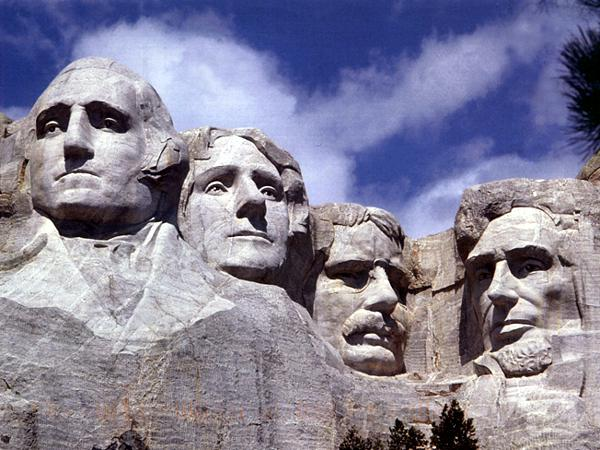
\includegraphics[width=4in]{MountRushmore.jpg}
\caption{The faces of Mount Rushmore---Public Domain}
\end{figure}

\index{information}
This ``special something'' is information.
Information is what distinguishes an empty hard disk from a full one.
Information is the difference between random scribbling and carefully printed prose.
Information is the difference between car parts strewn over a lawn, and a working truck.

\index{Shannon information|see{complexity, metrics, Shannon information}}
\index{complexity!metrics!Shannon information}
While humans operate using an intuitive concept of information, attempts to develop a theory of information have thus far fallen short of the intuitive concept.
Claude Shannon developed what its today known as Shannon information theory \citep{Shannon1948}.
Shannon's concern was studying the problem of communication, that of sending information from one point to another.
However, Shannon explicitly avoided the question of the meaningfulness of the information being transmitted, thus not quite capturing the concept of information as defined in this paper.
In fact, under Shannon's model a random signal has the highest amount of information, the precise opposite of the intuitive concept.

\index{algorithmic information theory}
Another model of information is that of algorithmic information theory \citep{Chaitin1966, Solomonoff1960, Kolmogorov1968a}.
\index{Kolmogorov complexity|see{complexity, metrics, Kolmogorov complexity}}
\index{complexity!metrics!Kolmogorov complexity}
Techniques such as Kolmogorov complexity measure the complexity of an object as the minimum length computer program required to recreate the object; Chaitin refers to such minimum length programs as \textit{elegant} \citep{Chaitin2002}.
As with Shannon information, random noise is the most complex because it requires a long computer program to describe.
In contrast, simple patterns are not complex because a short computer program can describe the pattern.
But neither simple patterns nor random noise are considered conceptual information.
As with Shannon information, there is a disconnect between Kolmogorov complexity and conceptual information.

Other models are based on algorithmic information theory, but also take into account the computational resources required for the programs being run.
\index{complexity!metrics!Levin complexity}
Levin complexity adds the log of the execution time to the complexity of the problem \citep{Levin1976}.
\index{complexity!metrics!logical depth}
\index{logical depth|see{complexity, metrics, logical depth}}
\textit{Logical depth}, on the other hand, is concerned with the execution time of the shortest program \citep{Bennett1988}.
There is a class of objects which are easy to describe but expensive to actually produce.
It is argued \citep{Bennett1988} that objects in this class must have been produced over a long history.
Such objects are interesting, but do not seem to capture the intuitive concept of information in its entirety.
English text or Mount Rushmore correspond to what is usually considered as information, but it is not clear that they can be most efficiently described as long running programs.

\index{complexity!metrics!specified complexity}
\index{specified complexity|see{complexity, metrics, specified complexity}}
\index{chance}
\index{necessity}
\index{agency}
\index{intelligence}
One approach to information is \textit{specified complexity} as expressed by Dembski \citep{Dembski1998}.
Dembski's concern is that of detecting design, the separation of that which can be explained by chance or necessity from that which is the product of intelligence. 
In order to infer design, an object must be both complex and specified.
Complexity refers, essentially, to improbability.
The probability of any given object depends on the chance hypothesis proposed to explain it.
Improbability is a necessary but not sufficient condition for rejecting a chance hypothesis.
Events which have a high probability under a given chance hypothesis do not give a reason to reject that hypothesis.

\index{specification}
Specification is defined as conforming to an independently given pattern.
The requirement for the pattern to be independent of the object being investigated is fundamental.
Given absolute freedom of pattern selection, any object can be made to seem specified by selecting that object as the pattern.
It is not impressive to hit a bullseye if the bullseye is painted on after the arrow has hit the wall.
It is impressive to hit the bullseye if the bullseye was painted before the arrow was fired.

\index{self-replication}
Investigators are often not able to choose the target prior to investigating the object.
For example, life is a self-replicating process, and it would seem that an appropriate specification would be self-replication.
Self-replication is what makes life such a fascinating area of investigation as compared to rocks.
Human beings know about self-replication \emph{because of} their knowledge of life, not as an independent fact.
Therefore, it does not qualify as an independent specification.
% If we did not already have examples of self-replicating entities, we would not have picked as the specification.

The same is true of almost any specification in biology.
It is tempting to consider flight a specification, but the pattern of flight would only be defined because flying animals have been observed.
As with life in general, specific features in biology cannot be specified independently of the objects themselves.

\index{specification|(}
\index{complexity!metrics!conditional Kolmogorov complexity}
\index{complexity!metrics!algorithmic specified complexity}
\index{algorithmic specified complexity|see{complexity, metrics, algorithmic specified complexity}}
The concept of specification has been criticized for being imprecisely defined and unquantifiable.
It has also been charged that maintaining the independence of the patterns is difficult.
But specification has been defined in a mathematically rigorous manner in several different ways \citep{Dembski1998, Dembski2002, Dembski2005a}.
Kolmogorov complexity, or a similar concept, is a persistent method used in these definitions.
Our goal is to present and defend a simple measure of specification that clearly alleviates these concerns.
Towards this end, this paper proposes to use \textit{conditional Kolmogorov complexity} to quantify the degree of specification in an object.
Conditional Kolmogorov complexity can then be combined with complexity as a measurement of specified complexity. This approach to measuring specified complexity is called \textit{algorithmic specified complexity}.

As noted, Kolmogorov complexity has been suggested as a method for measuring specification.
The novelty in the method presented in this paper is the use of conditional Kolmogorov complexity.
However, this paper also elucidates a number of examples of algorithmic compressibility demonstrating wider applicability than is often realized.

\section{Method}

\subsection{Kolmogorov}

\index{complexity!metrics!Kolmogorov complexity|(}
Kolmogorov complexity is a method of measuring information.
It is defined as the minimum length computer program, in bits, required to produce a binary string.
\begin{equation}
    K(X) = \min_{U(p,) = X \mid p \in P} |p|
\end{equation} where
\begin{itemize}
    \item $K(X)$ is the Kolmogorov complexity of X
    \item $P$ is the set of all possible computer programs
    \item $U(p,)$ is the output of program $p$ run without input
\end{itemize}
The definition is given for producing binary strings.

Kolmogorov complexity measures the degree to which a given bitstring follows a pattern.
The more a bitstring follows a pattern, the shorter the program required to reproduce it.
In contrast, if a bitstring exhibits no patterns, it is simply random, and a much longer program will be required to produce it.

\index{bitstrings}
Consider the example of a random binary string, {\tt 100100000010100000001010}.
It can be produced by the following Python program:

\begin{figure}[H]
\begin{mdframed}
\begin{verbatim}
    print '100100000010100000001010'
\end{verbatim}
\end{mdframed}
\caption{A Python program to produce an unpatterned bit string}
\end{figure}

In contrast, the string {\tt 000000000000000000000000} can be produced by

\begin{figure}[H]
\begin{mdframed}
\begin{verbatim}
    print '0' * 24
\end{verbatim}
\end{mdframed}
\caption{A Python program to produce a patterned bit string}
\end{figure}

Both strings are of the same length, but the string following a pattern requires a shorter program to produce,
thus a technique exists for measuring the degree to which a binary string follows a pattern.

Specification is defined as following an independently given pattern.
Kolmogorov complexity provides the ability to precisely define and quantify the degree to which a binary string follows a pattern.
Therefore, it seems plausible that a specification can be measured using Kolmogorov complexity.
The more compressible a bitstring, the more specified it is.

However, Kolmogorov complexity seems unable to capture the entirety of what is intended by specification.
Natural language text is not reducible to a simple pattern; however, it is an example of specification.
The design of an electronic circuit should also be specified, but it is not reducible to a simple pattern.
In fact, the cases of specification that Kolmogorov complexity seems able to capture are limited to objects which exhibit some very simple pattern.
But these are not the objects of most interest in terms of specification.
\index{complexity!metrics!Kolmogorov complexity|)}

\index{complexity!metrics!conditional Kolmogorov complexity}
There is also an extension of Kolmogorov complexity known as {\it conditional Kolmogorov complexity} which can be used \citep{Kolmogorov1968}.
With conditional Kolmogorov complexity, the program now has access to additional data as its input.
\begin{equation}
    K(X|Y) = \min_{U(p,Y) = X \mid p \in P} |p|
\end{equation} where $U(p,Y)$ is the output of running program $p$ with input $Y$.

In this calculation, the input provides additional data to the program.
As a result, the program is no longer restricted to exploiting patterns in the desired output but can take advantage of the information provided by the input.
\index{context}
Henceforth, this input is referred to as the {\it context}.

The use of context allows the measure to capture a broader range of specifications.
It is possible to describe many bitstrings by combining a short program along with the contextual information.
A useful range of specifications can be captured using this technique.
\index{specification|)}

\subsection{Algorithmic Specified Complexity}

\index{complexity!metrics!algorithmic specified complexity|(}
The following formula for algorithmic specified complexity (ASC) combines the measurement of specification and complexity.
\begin{equation}
    \label{ASC}
    A(X,C,p) = -\log p(X) - K(X|C)
\end{equation} where
\begin{itemize}
    \item $X$ is the bitstring being investigated
    \item $C$ is the context as a bitstring
    \item $p$ is the probability distribution which it is supposed that $X$ has been selected from
    \item $p(X)$ is the probability of $X$ occurring according to the chance hypothesis under consideration
\end{itemize}
Since high compressibility corresponds to specification, the compressed length of the string is subtracted.
Thus, high improbability counts for specified complexity, but incompressible strings count against it.

For this number to become large requires $X$ to be both complex (i.e., improbable) and specified (i.e., compressible).
Failing on either of these counts will produce a low or negative value.
Since Kolmogorov complexity can, at best, be upper bounded, the ASC can, at best, be lower bounded.

At best this measure can reject a given probability distribution.
It makes no attempt to rule out chance-based hypotheses in general.
However, it can conclude that a given probability distribution does a poor job in explaining a particular item.
The value of ASC gives a measure of the confidence available for rejecting a chance hypothesis.

\subsection{Functionality}

\index{functionality}
Perhaps the most interesting form of specification is that of functionality.
It is clear that machines, biological structures, and buildings all have functionality,
but quantifying that functionality in an objective manner has proven difficult.
However, ASC provides the ability to do this.

Any machine can be described in part by tests that it will pass:
The functionality of a car can be tested by seeing whether it accelerates when the gas or brake pedals are pushed;
the functionality of a cell by seeing whether it self-replicates.
A test, or a number of tests, can be defined to identify the functionality of an object. 
The existence of a test supplies the ability to compress the object.
Consider the following pseudocode program.

\begin{figure}[H]
\begin{mdframed}
\begin{verbatim}
counter = 0
for each possible building design
    if building won't fall over
        counter += 1
        if counter == X
             return building design
\end{verbatim} 
\end{mdframed}
\caption{A pseudocode program which uses a functional test to compress the specification of an object by its functionality}
\end{figure}
This program will output the design for a specific building based on a given value for $X$.
Different values of $X$ will produce different buildings.
But any building that will not fall over can be expressed by this program.
It may take a considerable amount of space to encode this number.
However, if few designs are stable, the number will take much less space than what would be required to actually specify the building plans.
Thus the stability of the building plan enables compression, which in turn indicates specification.

Kolmogorov complexity is not limited to exploiting what humans perceive as simple patterns.
It can also capture other aspects such as functionality.
Functionality can be described as passing a test.
As a result, functional objects are compressible.

\section{Examples}
\subsection{Natural Language}
\index{English text}
Consider the sentence: ``The quick brown fox jumps over the lazy dog.''
This sentence can be encoded as UTF-32, a system for encoding that allows the encoding of symbols from almost any alphabet.
Since each character takes 32 bits, the message will be encoded as a total of 1376 bits.
In this example, the context will be taken to be the English alphabet along with a space.
This is a minimal level of information about the English language.

To specify one of the 27 characters requires $\log_2 27$ bits. 
To specify the 43 character in the sentence will thus take $43 \log_2 27$ bits.
The number of characters are recorded at $2 \log_2 43 \approx 10.85$ bits. 
\footnote{A more compact representation for numbers is available. See the $log^*$ method in \citet{Cover2006}.}
Altogether, the specification of the message requires $43 \log_2 27 + 2 \log_2 43 \approx 215.32$ bits. 


However, in order to actually give a bound for Kolmogorov complexity, the length of the computer program which interprets the bits must also be included.
Here is an example computer program in Python which could interpret the message
\begin{figure}[H]
\begin{mdframed}
\begin{verbatim}
    print ''.join(alphabet[index] for index in encoded_message)
\end{verbatim}
\end{mdframed}
\caption{An example Python program to interpret the encoded message}
\end{figure}

This assumes that the alphabet and encoded message are readily available and in a form amenable to processing within the language.
It may be that the input has to be preprocessed, which would make the program longer.
Additionally, the length of the program will vary heavily depending on which programming language is used.
However, the distances between different computers and languages only differs by a constant \citep{Cover2006}.
As a result, it is common practice in algorithmic information theory, to discount any actual program length and merely include that length 
as a constant, $c$. 
Consequently, the conditional Kolmogorov complexity can be expressed as 
\begin{equation}
    \label{kc.alpha}
    K(X|C) \leq 215.32 \mbox{ bits} + c \mbox{.}
\end{equation}
The expression is less than rather than equal because it is possible that an even more efficient way of expressing the sentence exists.
However, at least this efficiency is possible.

The encoded version of the sentence requires 32 bits for each character, giving a total of 1376 bits.
Using a simplistic probability model, supposing that each bit is generated by the equivalent of a coin flip,
the complexity, $-\log P(X)$, would be 1376 bits.
Using equation~\ref{ASC},
\begin{equation}
    A(X,C,p) = -\log(p) - K(X|C) \geq 1376 \mbox{ bits} - 215.32 \mbox{ bits} - c  = 1160.68 \mbox{ bits} - c \mbox{.}
\end{equation}
This shows 1166 bits of algorithmic specified complexity by equation~\ref{ASC}.
Those 1166 bits are a measure of the confidence in rejecting the hypothesis that the sentence was generated by random coin flips.
The large number of bits gives a good indication that it is highly unlikely that this sentence was generated by randomly choosing bits.

The hypothesis that the sentence was generated by choosing random English letters can also be analyzed.
In this case the probability of this sentence can be calculated as
\begin{equation}
    P(X) = \left(\frac{1}{27}\right)^{43} \mbox{.}
\end{equation}
The complexity is then
\begin{equation}
    -\log P(X) = -\log \left(\frac{1}{27}\right)^{43} = 43 \log 27 \approx 204.46 \mbox{ bits,}
\end{equation}
in which case the algorithmic specified complexity becomes
\begin{equation}
    A(X,C,p) = - \log p(X) - K(X|C) \geq 204.46 \mbox{ bits} - 215.32 \mbox{ bits} - c = -10.85 \mbox{ bits} - c \mbox{.}
\end{equation}
The negative bound suggests no reason to suppose that this sentence could not have been generated by a random choice of English letters.
The bound is negative as a result of two factors.
In the specification, $10.85$ bits were required to encode the length.
On the other hand, the probability model assumes a length.
Hence, the negative bits indicate information which the probability model had, but was not provided in the context.
Since the only provided context is that of English letters, this is not a surprising result.
No pattern beyond that explained by the probability model is identified.

The context can also be expanded.
\index{dictionary}
Instead of providing the English alphabet as the context, the word list of the Oxford English Dictionary can be used \citep{Oxford2012}.
In the second edition of that dictionary there were 615,100 word forms defined or illustrated.
For the purpose of the alphabet context, each letter is encoded as a number corresponding to that character.
In this case, a number corresponding to words in the dictionary is chosen.
Thus the number of bits required to encode the message using this context can be calculated:
\begin{equation}
    \label{kc.dict}
    K(X|C) \leq 9 \log_2  615,100 + 2 \log_2 9 + c \approx 179.41 + c \mbox{.}
\end{equation}
Access to the context of the English dictionary allows much better compression than simply the English alphabet as comparing equations~\ref{kc.alpha} and ~\ref{kc.dict} shows.

Using equation~\ref{ASC} yields
\begin{equation}
    A(X,C,p) = - \log p(X) - K(X|C) \geq 204.46 \mbox{ bits} - 179.41 \mbox{ bits} - c = 25.05 \mbox{ bits} - c \mbox{.}
\end{equation}
This provides confidence to say this sentence was not generated by randomly choosing letters from the English alphabet.

It is possible to adopt a probability model that selected random words from the English language.
Such a probability model would explain all of the specification in the sentence.
It is also possible to include more information about the English language such that the specification would increase.

This technique depends on the fact that the numbers of words in the English language is much smaller then the number of possible combinations of letters.
If the dictionary contained every possible combination of letters up to some finite length, it would not allow compression, and thus be of no help to finding evidence of specification.
A language where all possible combinations of letters were valid words could still show specification, but another technique would have to be used to allow compression.

But one could also use a much smaller dictionary.
A dictionary of 10 words would be sufficient to include all the words in this sentence.
The ASC formula would give a much smaller compressed bound:
\begin{equation}
    K(X|C) \leq 9 \log_2 10 + 2 \log_2 9 \approx 36.24 \mbox{ bits.}
\end{equation}
This is a reduction of over 100 bits from equation~\ref{kc.dict}.
Because the sentence is much more closely related to the context
it takes about 16 bits less to encode each word when the dictionary is this small.
In other words, it requires much less additional information to use the context when it is closely related to the message.

But it is possible to include words not included in the dictionary.
The program would have to fall back on spelling the word one letter at a time.
Only the bounds of the ASC can be computed.
It is always possible a better compression exists, i.e.,\ the object could be more specified than first realized.

\subsection{Random Noise}
\index{randomness}
While natural language is an example of something that should be specified, random noise is an example of something which should not.
Consider a random bitstring containing 1000 bits, where each bit is assigned with equal probability 1 or 0.
Since randomness is incompressible, calculating the Kolmogorov complexity is easy.
The only way of reproducing a random bitstring is to describe the whole bitstring.
\begin{equation}
    K(X) \leq 2 \log_2 1000 + 1000 + c \approx 1020 \mbox{ bits} + c
\end{equation}
The probability of each bitstring is $2^{-1000}$, and thus the complexity will be 1000 bits.
Calculating the ASC:
\begin{equation}
    A(X,C,p) = - \log p(X) - K(X|C) \geq 1000 \mbox{ bits} - 1020 \mbox{ bits} - c = -20 \mbox{ bits} - c \mbox{.}
\end{equation}
As expected, the ASC is negative, and there is therefore no evidence of patterns in the string that are not explained by the probability model.

However, consider also the case of a biased distribution.
That is, 1 and 0 are not equally likely.
Instead, a given bit will be 1 two thirds of the time, while 0 only one third of the time.
The entropy of each bit can be expressed as
\begin{equation}
    H(X_i) = - \frac{1}{3} \log_2 \frac{1}{3} - \frac{2}{3} \log_2 \frac{2}{3} \approx 0.6365 \mbox{ bits}
\end{equation} for any $i$.
The entropy of a bit is the number of bits required in an optimal encoding to encode each bit.
This means the whole sequence can be described as
\begin{equation}
    K(X) \leq 2 \log_2 1000 + 1000*H(X_i) + c \approx 656.5 \mbox{ bits} +c \mbox{.}
\end{equation}
Using the uniform probability model, the complexity is still 1000 bits and
\begin{equation}
    A(X,C,p) = - \log p(X) - K(X|C) \geq 1000 \mbox{ bits} - 656.5 \mbox{ bits} - c = 343.3 \mbox{ bits} -c \mbox{.}
\end{equation}
This random sequence has a high bound of algorithmic specified complexity.
It is important to remember that the ASC bound only serves to measure the plausibility of the random model.
It does not exclude the existence of another more accurate model that explains the data.
In this case, using the actual probability model used to generate the message yields
\begin{equation}
    -\log_2(p) = H(X_i) * 1000 \approx 636.5 \mbox{ bits.}
\end{equation}
and the resulting ASC:
\begin{equation}
    A(X,C,p) = - \log p(X) - K(X|C) \geq 636.5 \mbox{ bits} - 656.5 \mbox{ bits} - c = -20 \mbox{ bits} -c \mbox{.}
\end{equation}
The bound of ASC provides reason to reject a uniform noise explanation for this data, but not the biased coin distribution.

\index{ballot rigging}
Dembski \citep{Dembski1998} has considered the example of ballot rigging where a political party is almost always given the top billing on the ballot listing candidates.
Since the selection is supposed to be chosen on the basis of a fair coin toss, this is suspicious.
ASC can quantify this situation.
The outcome can be described by giving the numbers of heads and tails, follow by the same representation as for the biased coin distribution.
\begin{equation}
    K(X) \leq 2 \log X_h + 2 \log X_t + \log {X_t + X_h \choose X_h} + c
\end{equation} where $X_h$ is the number of heads, $X_t$ is the number of tails
Assuming a probability model of a fair coin yields
\begin{equation}
    -\log_2(p) = X_h + X_t \mbox{bits.}
\end{equation}
This results in the following:
\begin{align}
    A(X,C,p) &= X_h + X_t - 2 \log X_h -  2 \log X_t - \log {X_t + X_h \choose X_h} - c \nonumber \\
    &= X_h + X_t - \log \left( X_h^2 X_t^2 {X_t + X_h \choose X_h} \right) - c \mbox{.}
\end{align}
\begin{figure}
    \begin{center}
        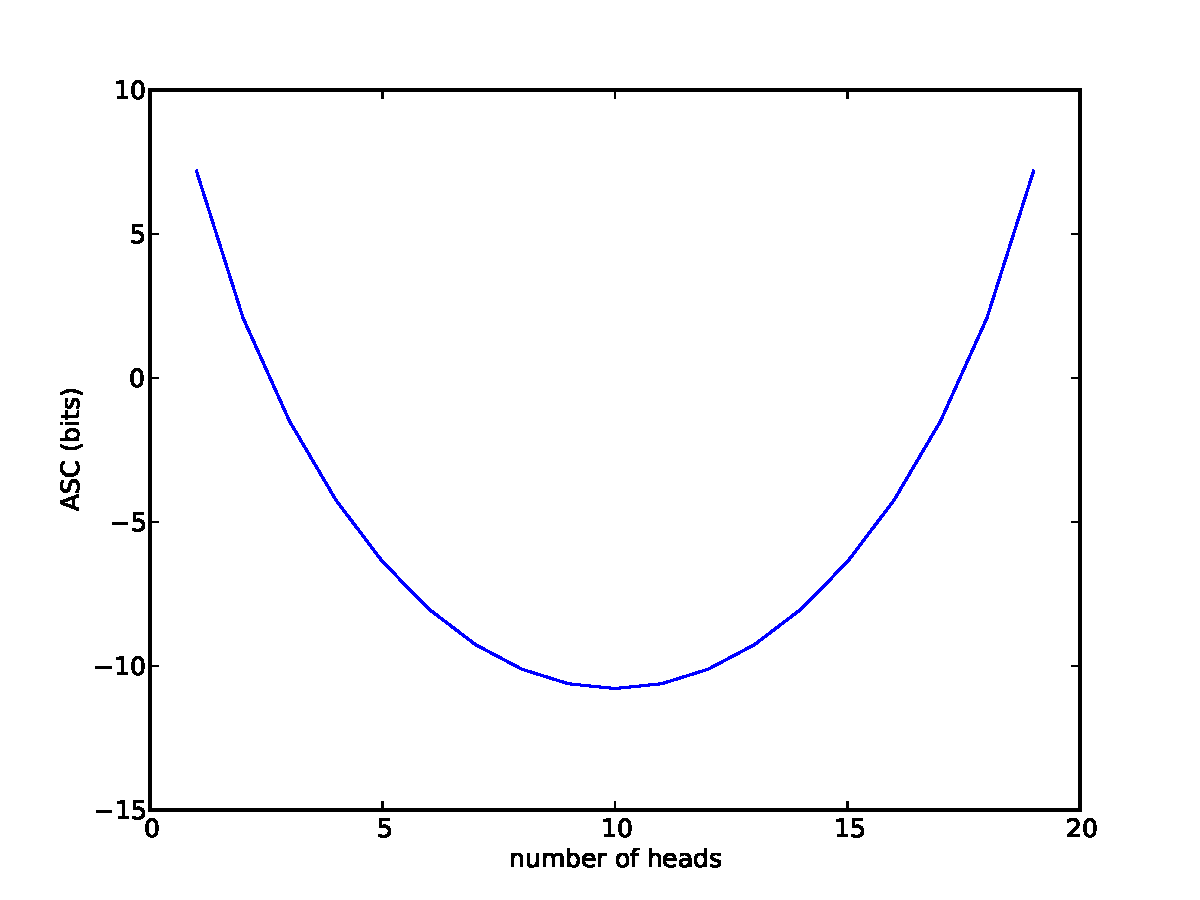
\includegraphics[width=.5\textwidth]{EwertCoin}
    \end{center}
    \caption{ASC for varyingly biased coin sequences and 20 coin tosses}
    \label{fig_coins}
\end{figure}
Figure~\ref{fig_coins} shows the result of plotting this equation for varying numbers of head and tails given 20 coin tosses.
As expected, for either high numbers of tails or high number of heads, the bound of ASC is high.
However, for an instance which looks like a random sequence, the ASC is minimized.


\subsection{Playing Cards}

\index{poker}\index{cards}
Another interesting case is that of playing cards in poker.
In playing cards, if the distribution is not uniform, somebody is likely cheating.
For the purpose of investigating card hands, a uniform random distribution over all five-card poker hands is assumed.

\begin{table}
    \begin{center}
    \begin{tabular}{ll}
        Name & Frequency \\
        \hline
        Royal Flush & 4 \\
        Straight Flush & 36 \\
        Four of a Kind & 624 \\
          Full House & 3744 \\
               Flush & 5108 \\
            Straight & 10200 \\
     Three of a Kind & 54912 \\
            Two Pair & 123552 \\
            One Pair & 1098240 \\
            None & 1302540 \\
    \end{tabular}
    \end{center}
    \caption{Poker hand frequency}
    \label{poker}
\end{table}
In the game of poker,
a poker hand is made up of 5 cards.
Some categories of hands are rarer then others.
Table~\ref{poker} shows the frequency of the different hands.

Given a uniform distribution, every poker hand has the same probability, and thus the same complexity.
There are 2,598,960 possible poker hands. 
For a single hand, this yields a complexity of
\begin{equation}
    -\log_2{p(X)} = -\log_2(\frac{1}{2,598,960}) \approx 21.3 \mbox{ bits.}
\end{equation}
While the probability of every poker hand is the same, the Kolmogorov complexity is not.
\index{royal flush}
To describe a royal flush requires specifying that it is a royal flush, and which suit it is in.
However, describing a pair requires specifying the paired value as well as both suits in addition to the three cards not involved in the pair.
In general, describing a hand requires specifying the type of hand, and which particular hand of all the possible hands of that type.
This can be used to calculate the conditional Kolmogorov complexity for the hand.
\begin{equation}
    \label{kc.card}
    K(H_i|C) \leq \log_2 10 + \log_2 |H| + c \mbox{.}
\end{equation} where $10$ is the number of types of hands. $H$ is the set of all hands of a particular type, and $H_i$ is a particular hand in that set.

There are 1,098,240 possible pairs.
Putting this in Equation~\ref{kc.card} gives:
\begin{equation}
    K(H_i|C) \leq \log_2 10 + \log_2 |H| + c \approx 23.39 \mbox{ bits} + c \mbox{.}
\end{equation}
On the other hand, describing a pair without using the context gives
\begin{equation}
    K(H_i|C) \leq \log_2 2,598,960 + c \approx 21.3 \mbox{ bits} + c \mbox{.}
\end{equation}
Single pairs are so common that the space required to record that it was a pair is more than the space required to record the duplicate card straightforwardly. 
Accordingly, the best approach is to take the minimum of the two methods
\begin{equation}
    K(H_i|C) \leq \min(\log_2 10 + \log_2 |H|, \log_2 2,598,960) + c \mbox{.}
\end{equation}

\begin{table}
    \begin{center}
    \begin{tabular}{lllll}
        Name & Frequency & Complexity & Compressed Length & ASC \\
        Royal Flush&4&21.310&5.322&15.988 \\
Straight Flush&36&21.310&8.492&12.818 \\
Four of a Kind&624&21.310&12.607&8.702 \\
Full House&3,744&21.310&15.192&6.117 \\
Flush&5,108&21.310&15.640&5.669 \\
Straight&10,200&21.310&16.638&4.671 \\
Three of a Kind&54,912&21.310&19.067&2.243 \\
Two pair&123,552&21.310&20.237&1.073 \\
One pair&1,098,240&21.310&21.310&0.000 \\
None&1,302,540&21.310&21.310&0.000 \\

    \end{tabular}
    \end{center}
    \caption{The ASC of the various poker card hands}
    \label{asc.hands}
\end{table}
Table~\ref{asc.hands} shows the ASC for the various poker hands.
Rare hands have large ASC, but common hands have low ASC.
This parallels expectations, because with a rare hand one might suspect cheating, but with a common hand one will not.

\index{trump}
In other card games, a card is turned over after hands have been dealt to determine trump.
The suit of the card is taken to trump for that round of the game.
If the same suit is repeatedly chosen as trump, someone may ask what the odds are for that to occur.
This question can be difficult to answer because every possible sequence of trump suits is equally likely.
Yet, it is deemed unusual that the same suit is a trump repeatedly.
Algorithmic specified complexity allows this to be modeled.

The suits are represented as a bit sequence, using two bits for each suit.
\begin{equation}
    K(X) = \log_2 4 + \log_2 H + c = 2 + \log_2 H + c
\end{equation} where 4 is the number of suits, and H is the number of hands played.
The complexity of the sequence is 
\begin{equation}
    -\log P(X) = 4^\frac{-|X|}{2} = 2H \mbox{.}
\end{equation}
The ASC is then
\begin{equation}
    ASC(X,p) = 2H - 2 - \log_2 H - c \mbox{.}
\end{equation}
Note that this equation becomes $-c$ when $H=1$.
A pattern repeating once is no pattern at all, and does not provide specification.
\begin{figure}
    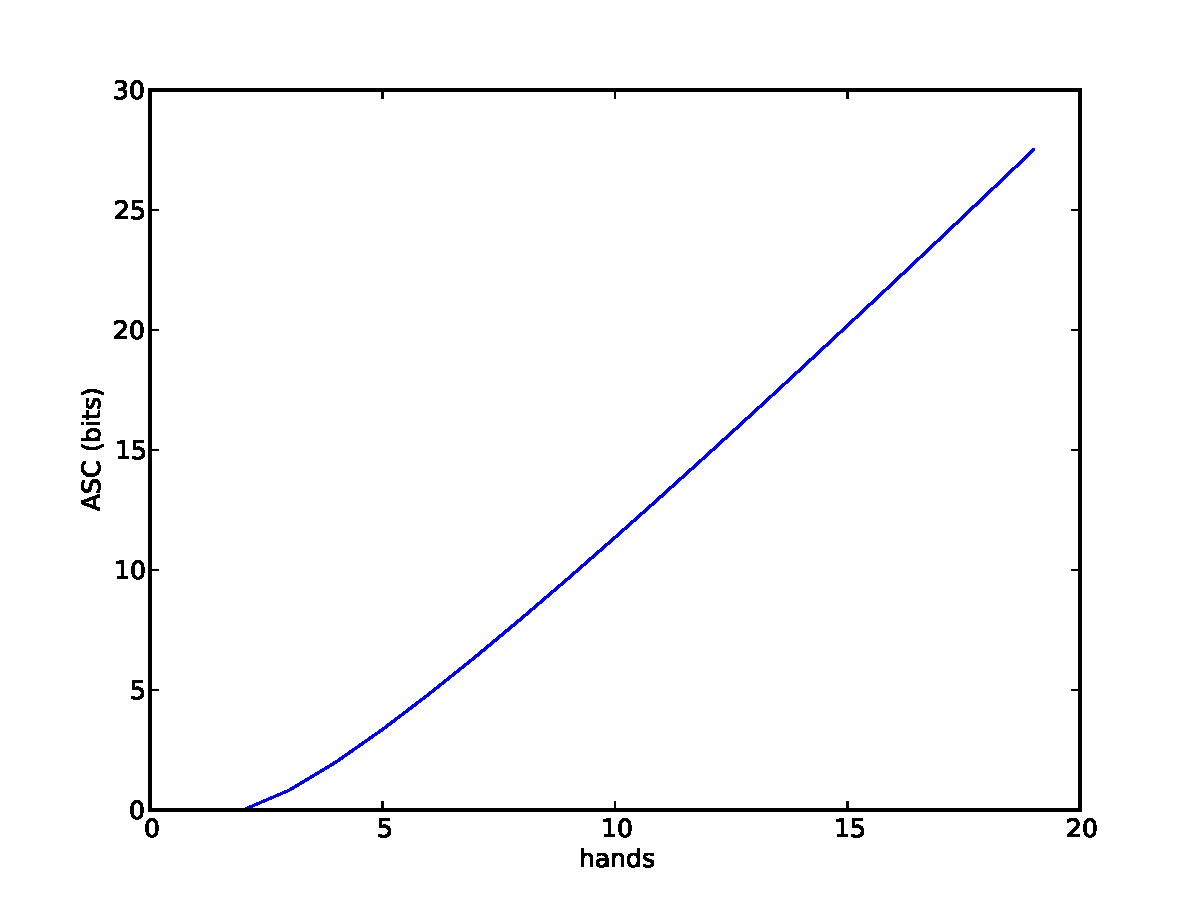
\includegraphics[width=\textwidth]{EwertRepeat}
    \caption{A plot of ASC for getting the same suit repeatedly}
    \label{suit.plot}
\end{figure}
Figure~\ref{suit.plot} shows the ASC for increasing numbers of hands.
The more times the same suit is chosen as trump, the larger the number of bits of ASC.
The same trump for many rounds becomes less and less probable.
\index{complexity!metrics!algorithmic specified complexity|)}

\subsection{Folding Proteins}
\label{sec_folding}

\index{proteins!folding}
In biology, an important prerequisite to a protein being functional is that it folds.
The fraction of all possible protein sequences that fold has been estimated: ``the overall prevalence of sequences performing a specific function by any domain-sized fold may be as low as 1 in $10^{77}$'' \citep{axe2004}.

A program can be created which uses the laws of physics to output a particular foldable protein.
\begin{figure}[H]
\begin{mdframed}
\begin{verbatim}
for all proteins of length L
    run protein in a physics simulator
    if protein folds
        add to list of folding proteins
output the Xth protein from the list
\end{verbatim}
\end{mdframed}
\caption{A pseudocode program which uses a functional specification to compress the specification of a protein}
\end{figure}

Given different choices of $L$ and $N$, this program will output any particular folding protein.
This means that the protein can be described by providing those two numbers.  Thus, the conditional Kolmogorov complexity can be calculated using these two numbers.
\begin{equation}
    K(X|C) = 2 \log_2 L + \log_2 F_L + c
\end{equation} where $C$ is the context, in this case the law of physics,
and $F_L$ is the number of folding proteins of length $L$.
Taking Axe's estimate \citep{axe2004}, and assuming simplistically that it applies for all lengths of proteins:
\begin{equation}
    F_L = 10^{-77} 4^L 
\end{equation}
\begin{equation}
    \log F_L = -77 \log 10 + L \log 4
\end{equation}
so
\begin{equation}
    K(X|C) = 2 \log_2 L + \log_2 F_L + c = 2 \log_2 L + -77 \log 10  + L \log 4 \mbox{.}
\end{equation}

\index{DNA}\index{protein}
The probability model will be chosen by supposing that each base along the DNA chain for the gene encoding the protein is uniformly chosen.
It should be emphasized that according to the Darwinian model of evolution, the bases are not uniformly chosen.
This supposition only serves to test a simplistic chance model of protein origin.
The probability can be calculated as
\begin{equation}
    -\log_2 \Pr(X) =  -\log_2 4^{-L} = L \log_2 4 \mbox{.}
\end{equation}
Caution should be used in applying this formula.
It assumes that the proportion of functional proteins is applicable for all lengths, and implies that a fractional number of proteins fold.

\index{complexity!metrics!algorithmic specified complexity}
Finally calculating the ASC,
\begin{align}
    ASC(X,p) &= L \log 4 - 2 \log_2 L + 77 \log_2 10 - L \log_2 4 - c \nonumber \\
    &= - 2 \log_2 L + 77 \log_2 10 - c \mbox{.}
\end{align}
The final bound for ASC depends little on the length of the protein sequence which only comes to play in the logarithmic term.
The significant term is the $77 \log_2 10 \approx 255.79 \mbox{ bits}$.
Thus, there is good reason to believe that folding sequences were not generated randomly from a uniform distribution.

\subsection{Functional Sequence Complexity}
\index{functional sequence complexity|see{complexity, metrics, functional sequence complexity}}
\index{complexity!metrics!functional sequence complexity|(}
\index{complexity!metrics!algorithmic specified complexity|(}
Kirk Durston et al. have defined the idea of {\it functional sequence complexity} \citecustom{Durston2007}{Durston, Chiu, Abel, \& Trevors}.
Functional sequence complexity is related to a special case of algorithmic specified complexity.

A protein is made from a sequence of amino acids.
Some sequences have functionality, and some do not.
The case considered in section \ref{sec_folding} above of folding is one particular case.
Perhaps more interesting is considering the case of various proteins which perform useful biological functions.

Let $\Omega$ be the set of all proteins.
Let $F$ be the set of all proteins which pass a functionality test.
Let $f(x)$ be a probability distribution over $F$.
Both $F$ and $f(x)$ can be produced by a simple algorithm using a functionality test on each element of $\Omega$.
Consequently, $F$ and $f(x)$ can be described using a constant program length.

Consider the average for ASC over all elements in $F$.
\begin{align}
    \label{ASC.FSC.1}
    \sum_{x \in F} f(x) A(x,C,p) 
    &= \sum_{x \in F} f(x) (-\log p(x) - K(x|C))  \nonumber \\
    &= \sum_{x \in F} -f(x)\log p(x) - \sum_{x \in F} f(x) K(x|C))
\end{align}

Any element $x$ can be described given the probability distribution and $\log f(x) \mbox{ bits}$.
Given that $f(x)$ and $F$ can be calculated with a constant program, the conditional Kolmogorov complexity can be calculated as
\begin{equation}
    K(x|C) \leq \log -f(x) + c  \mbox{.}
\end{equation}
Place this into equation~\ref{ASC.FSC.1}.
\begin{equation}
    \sum_{x \in F} f(x) A(x,C,p) 
    \geq \sum_{x \in F} -f(x)\log p(x) - \sum_{x \in F} - f(x) \log f(x) - \sum_{x \in F} c
\end{equation}
The middle term is recognized as the Shannon entropy.
\begin{equation}
    \sum_{x \in F} f(x) A(x,C,p) 
    \geq \sum_{x \in F} -f(x) \log p(x) - H(f) - c \sum_{x \in F} f(x)
\end{equation}
If the distribution $p$ is uniform, $p(x) = \frac{1}{|\Omega|}$,
\begin{equation}
    \sum_{x \in F} f(x) A(x,C,p) 
    \geq \log_2 |\Omega| \sum_{x \in F} f(x) - H(f) - c \sum_{x \in F} f(x)  \mbox{.}
\end{equation}
The two summations over F, are summations over a probability distribution and therefore 1.
\begin{equation}
    \sum_{x \in F} f(x) A(x,C,p) 
    \geq \log_2 |\Omega| - H(f) - c 
\end{equation}
Equation 5 in Durston's work, adjusting for notation is
\begin{equation}
    \log |\Omega| - H(f)  \mbox{.}
\end{equation}
This equation derives from making the same uniformity assumption made above.
Thus, for the uniform probability distribution case,
\begin{equation}
    \sum_{x \in F} (f(x) A(x,C,p) ) + c
    \geq \log |\Omega| - H(f)  \mbox{.}
\end{equation}
This establishes the relationship between ASC and FSC.
The difference is that the ASC is a lower bound and includes a constant.
This is the same constant as elsewhere: the length of the program required to describe the specification.
\index{complexity!metrics!functional sequence complexity|)}
\index{complexity!metrics!algorithmic specified complexity|)}

\section{Objections}

\subsection{Natural Law}
\index{natural law}
\index{compressibility}
\index{information}
We have argued that compressibility in the presence of context is a necessary condition for information.
This is in contrast to others who have argued that lack of compressibility is a necessary condition for information \citep{Abel2005}.
But compressible objects lack complexity.
Because a compressible object is describable as some simple pattern, it is amenable to being produced by a simple process.
Many objects in the real world follow simple patterns.
Water tends to collect at lower elevations.
Beaches follow a sloping pattern.
Sparks fly upwards.
But these patterns are the result of the operation of simple law-like processes.
Even if the explanations for these patterns were unknown, the simplicity of the pattern suggests that some simple explanation existed.

\index{redundancy}
\index{patterns}
\index{algorithms}
\index{compressibility}
The premise behind this use of compressibility is that it identifies what human would see as simple patterns.
Abel writes: ``A sequence is compressible because it contains redundant order and patterns'' \citep{Abel2005}.

The problem is that algorithms are very versatile and allow the description of many patterns beyond that which humans would see as patterns.
As has been shown by the various examples in this paper, many objects which do not exhibit what humans typically identify as redundant order and patterns are in fact compressible.
Significantly, functionality actually allows compressibility.
Contrary to what Abel states, functional sequences are compressible by virtue of the functionality they exhibit.
All of the sequences that Abel holds to be mostly incompressible are actually compressible.

But are compressible objects amenable to explanation by simple processes?
Do all compressible objects lack complexity?
If this were true, it would be problematic for algorithmic specified complexity because all specified objects would also not be complex, and no object would ever be both specified and complex.
But many compressible objects do not appear amenable to explanation by a simple process.

As discussed, English text is compressible given a knowledge of the English language.
This does not somehow make it probable that English text will appear on a beach carved out by waves.
Ninety degree angles are very compressible; yet, they are not typically found in nature.
The existence of an explanation from the laws of nature does not appear to follow from compressibility.

\index{complexity!metrics!Kolmogorov complexity}
Kolmogorov complexity deliberately ignores how long a program takes to run.
It is only concerned with the length of the program's description.
A program may be short but take an astronomical amount of time to run.
Many of the specifications considered in this paper fall into that category.
These objects are compressible, but that compression does not give a practical way to reproduce the object.
But if there is no practical way to reproduce the object, there is no reason to suggest law-like processes as a plausible explanation.

\subsection{Context is Subjective}
\index{context}\index{subjectivity}
The ASC of any object will depend on the context chosen.
Any object can be made to have high ASC by using a specifically chosen context.
But this appears to be the way that information works.
If the authors, who do not understand Arabic, look at Arabic text, it appears to be no better then scribbling.
The problem is not that Arabic lacks information content, but that the reader is unable to identify it without the necessary context.
As a result, this subjectivity appears to capture something about the way information works in the human experience.

\index{specification}
As with specification, it is important that the context be chosen that is independent of the object under investigation.
While a specification will rarely be independent of the object under investigation, it is much easier to maintain this independence in the case of a context.

\subsection{Incalculability}
\index{incomputability}
It is not possible to calculate the Kolmogorov complexity of an object.
However, it is possible to upper-bound the Kolmogorov complexity and thus lower-bound the algorithmic specified complexity.
This means that something can be determined to be at least this specified, although the possibility that it is even more specified cannot be ruled out.
Therefore, even though detecting a specification cannot be achieved mechanically, it can be objectively identified when found.

%\section{Conclusions}
%
%\index{complexity!metrics!specified complexity}
%\index{complexity!metrics!algorithmic specified complexity}
%Dembski argued that information can be detected by looking for specified complexity.
%We propose that all or most forms of specification can be represented as algorithms, using Kolmogorov complexity.
%The shorter the algorithm, the more specified the object is.
%In order to measure a broader range of specification, we include the context and thus make use of conditional Kolmogorov complexity.
%We have defined the concept of Algorithmic Specified Complexity which takes into account the probabilistic complexity as well as the Kolmogorov complexity. 
%We have presented a number of examples showing how this can represent the specification in a variety of cases.
%We hope that this paper introduces discussion on the use of conditional Kolmogorov complexity as a method for measuring specification as well as the use of Algorithmic Specified Complexity.

\unnumberednotocsection{Acknowledgements}{Acknowledgements}

The approach of using compressibility as a measurement of specification was suggested to the authors by Eric Holloway.
The authors have attempted to extend the approach to apply to many more types of specifications.
The authors are grateful for his initial suggestion and answer to our initial objections to the idea.

\eandmbibliography{EwertLibrary}


%% FIXME - check use of n-dashes - shouldn't most of them just be hyphens?  Is it typesetting the hyphens correctly?
\eandmchapter{Using Turing Oracles}{Using Turing Oracles in Cognitive Models of Problem-Solving}{Jonathan Bartlett}{The Blyth Institute}

\begin{abstract}
\index{problem-solving}
\index{Turing Oracle}
\index{computation!theory}
\index{cognition}
At the core of engineering is human problem-solving.  Creating a cognitive model of the task of problem-solving is helpful for planning and organizing engineering tasks.  One possibility rarely considered in modeling cognitive processes is the use of Turing Oracles.  \citet{copeland1998} put forth the possibility that the mind could be viewed as an oracle machine, but never applied that idea practically.  Oracles enable the modeling of processes in the mind which are not computationally-based.  Using oracles resolves many of the surprising results of computational problem-solving which arise as a result of the Tractable Cognition Thesis and similar mechanistic models of the mind.  However, as research into the use of Turing Oracles in problem-solving is new, there are many methodological issues.
\end{abstract}

\section[Broad Views of Cognition]{Broad Views of Cognition and Their Historic Consequences in Cognitive Modeling}

\index{cognition}
\index{cognitive modeling}
\index{physicalism|see{cognition, metaphysics, physicalism}}
\index{cognition!metaphysics!physicalism}
In the philosophy of mind, three main overarching theories exist concerning how the mind works---physicalism, dualism, and emergentism.  These are ways of understanding cognitive processes in their broadest view.  Physicalism is the idea that there is nothing going on in the mind that is not describable through standard physical processes.  There may yet be physical processes that we do not currently understand or are even aware of, but, in the long run, there should not be anything involved in causal processes that is not physical and understandable through physics.  Some physicalists allow for the non-reduction of mental states to physical states, or at least an epistemological reduction, but they are all clear in the closed causality of the physical \citep{horgan1994}.

\index{cognition!metaphysics!dualism}
\index{dualism|see{cognition, metaphysics, dualism}}
Dualism is the primary contender for this area.\index{dualism}  Dualism is the idea that the mind and the body are not equivalent---that there exists at least some part of human cognition that is beyond what is describable by physics or using physical entities.  It holds that a reduction of the mind to brain physics does not capture the entirety of what the mind is doing.  It also says that there is a causal element being left out---that the mind, while not itself entirely physical, participates in the causal chain of human action.  In other words, it is not a purely passive element but has a causal role \citep{heart1994}.

\index{emergence|see{cognition, metaphysics, emergence}}
\index{cognition!metaphysics!emergence}
A third theory is emergentism.  Emergentism tries to split the line between physicalism and dualism.  However, it is a very fluid term and is difficult to distinctly identify.  Some forms of emergentism (especially ``weak emergence'' or ``epistemological emergence'') are essentially physicalism, while others (for instance, ``strong emergence'' or ``ontological emergence'') propose outside laws of emergence which transform the character of initial properties in certain configurations \citep{oconnorwong2012}.  Therefore, strong emergence tends to be essentially a form of dualism except that the dualistic properties are captured in a set of laws of emergence.  The question then is whether these laws themselves can be considered material.  Since the question posed in this study concerns whether or not physical causation is sufficient for an explanation, most views of emergence can be classified as either physicalist or dualist.

\index{cognition!metaphysics|(}
\index{metaphysics|see{cognition, metaphysics}}
Historically, aspects of cognition that were considered to be part of the non-physical mind were left unmodeled by dualists.  By contrast, the goal of physicalism is to force all phenomena into explicitly physical models, a process not easily accomplished.

To begin with, defining physicalism and dualism are not easy tasks. For a dualist to say that there is more than one mode of causation, at least one of those modes needs to be clearly and explicitly described.  Similarly, if a physicalist says that all causes are physical, such a statement is meaningless without a solid definition of what counts as physical and what does not \citep{stoljar2009}.

Several insufficient definitions of physicalism are often suggested. For example, one definition is that physicalism deals only with material causes.  However, no clear explanation is given as to what counts as a material cause.  Another definition is that physicalism deals only with observable phenomena.  This could have two meanings, both of which are problematic.  If it means that it deals only with things which can be observed directly, then this would remove most of modern physics from the physical---direct observation is not possible for atoms, molecules, forces, and the like.  If, on the other hand, the definition includes indirect observations, then there is no reason to suppose that only physical entities are observable.  It is precisely the contention of the dualists that there are non-physical modes of causation which have real effects in the world.  If dualism is true, then non-physical causes should be indirectly observable.  Therefore, observability can't be a distinguishing factor.  A third definition is that physical things are testable.  However, this fails for the same reason that the observable definition fails.  Testing simply means looking at observations, and determining whether or not they match the expectations of the theory.  Therefore, any observable phenomena should be testable in the same way.

\index{Turing, Alan}
\index{Godel@G\"{o}del, Kurt}
\index{Tractable Cognition Thesis}
\index{computability}
\index{Principle of Computational Equivalence}
\index{incomputability}
\index{cognition!metaphysics|)}
One distinguishing factor proposed by physicalists to distinguish between physical and non-physical behavior is computability.  With computability, physical processes are those whose results can (at least in theory) be calculated by computational systems, while non-physical processes are those which cannot.  This has been proposed by Iris van Rooij in his \textit{Tractable Cognition Thesis} as well as Stephen Wolfram in his \textit{Principle of Computational Equivalence} \citep{vanrooij2008, wolfram2002}.  By using this well-defined theory of computability and incomputability, developed in the early 20th century by G\"{o}del, Church, Turing, and others, it becomes at least possible to make meaningful statements about physical and non-physical processes.  In addition, because of the groundwork laid by the same pioneers of computability and incomputability, further advances can be made beyond
previous dualist conceptions of the mind which actually include non-physical elements in models of cognition.

\section[A Primer on Computability]{A Primer on Computability and Incomputability}

\index{incomputability}
Incomputability generally refers to the question of whether or not a given function can be computed given a set of operators.  So, for instance, given only the addition, subtraction, and summation operators, division cannot be computed.  However, given those same operators, a multiplication function can be computed.  

\index{self-reference}
One place where incomputability reigns is on self-referential questions.  There are numerous questions that can be asked about a set of mathematical operators which cannot be answered solely by the functions of the operators themselves.  For example, let's say you have a set of operators ($O$) and a list ($L$) of all of the valid functions that take a single value as a parameter, yield a single value as a result, are of finite length, and can be defined using the operators in $O$, listed in alphabetic order.  This is a countable infinity because each function in $L$ can be identified by an ordinal number, which is its index into the list.  Now, because all of $L$ are valid functions, there exists a function $F(x)$ which takes the function from $L$ at index $x$ and yields the value of that function with $x$ as the parameter.  The question is, is $F(x)$ in $L$?  

The answer, perhaps surprisingly, is no.  This means that defining $F(x)$ will require operators not in $O$.  Another example will help demonstrate why. Take another function, $G(x)$, which returns $F(x) + 1$.  If $F(x)$ is in $L$, then, $G(x)$ is also in $L$ (assuming that the addition operator is in $O$).  If $G(x)$ is at index $n$ of $L$ and has a result $r$ when computed using its own index (which is defined as $n$), by definition, since $n$ is the index of $G$, then $F(n)$ must return the same result as $G(n)$, which we have defined to be $r$.  However, the definition of $G(x)$ says that it must be $F(x) + 1$!  Since $F(n)$ returns $r$ and $G(n)$ returns $r$, this leads to a contradiction, because $r$ cannot be equal to $r + 1$.  Therefore, $F(x)$ cannot be computed using the operators in $O$.  This proof is quite independent of what operators exist in $O$, provided they are singly-valued and include the addition operator.  Thus, $F(x)$ is a true function of $x$, but is incomputable with fixed-length programs of operators in $O$.

\index{Church-Turing thesis}
Using the example given above, it seems that computability questions are based on the set of operators being used to define it.  This is largely true.  So, if computability is operator-dependent, how can it help us in the case of answering questions about the physicality of the process?  The Church-Turing thesis provides a solution, stating that all finitary mathematical systems are computationally equivalent to some Turing machine \citep{turing1937,turing1939}.\footnote{Turing machines are important because their functions can be explicitly described and their operations can be concretely implemented in the real world using machines, and as such they are both verifiable and unambiguous.  A Turing machine consists of four parts---an (theoretically) infinitely long tape (i.e., memory), a read/write head for the tape, a state register, and a fixed state transition table.  The only unimplementable feature of Turing machines is the requirement for an infinitely long tape.  However, in the absence of an infinite tape, we can at least detect when a given process requires more tape than we actually have.  One of the purposes of Turing machines was to make explicit what was meant by the terms ``algorithm,'' ``effectively calculable,'' and ``mechanical procedure.''  In other words, the original purpose of developing Turing machines was to delineate between what was calculable and what was not.}

\begin{figure}[H]
\centering
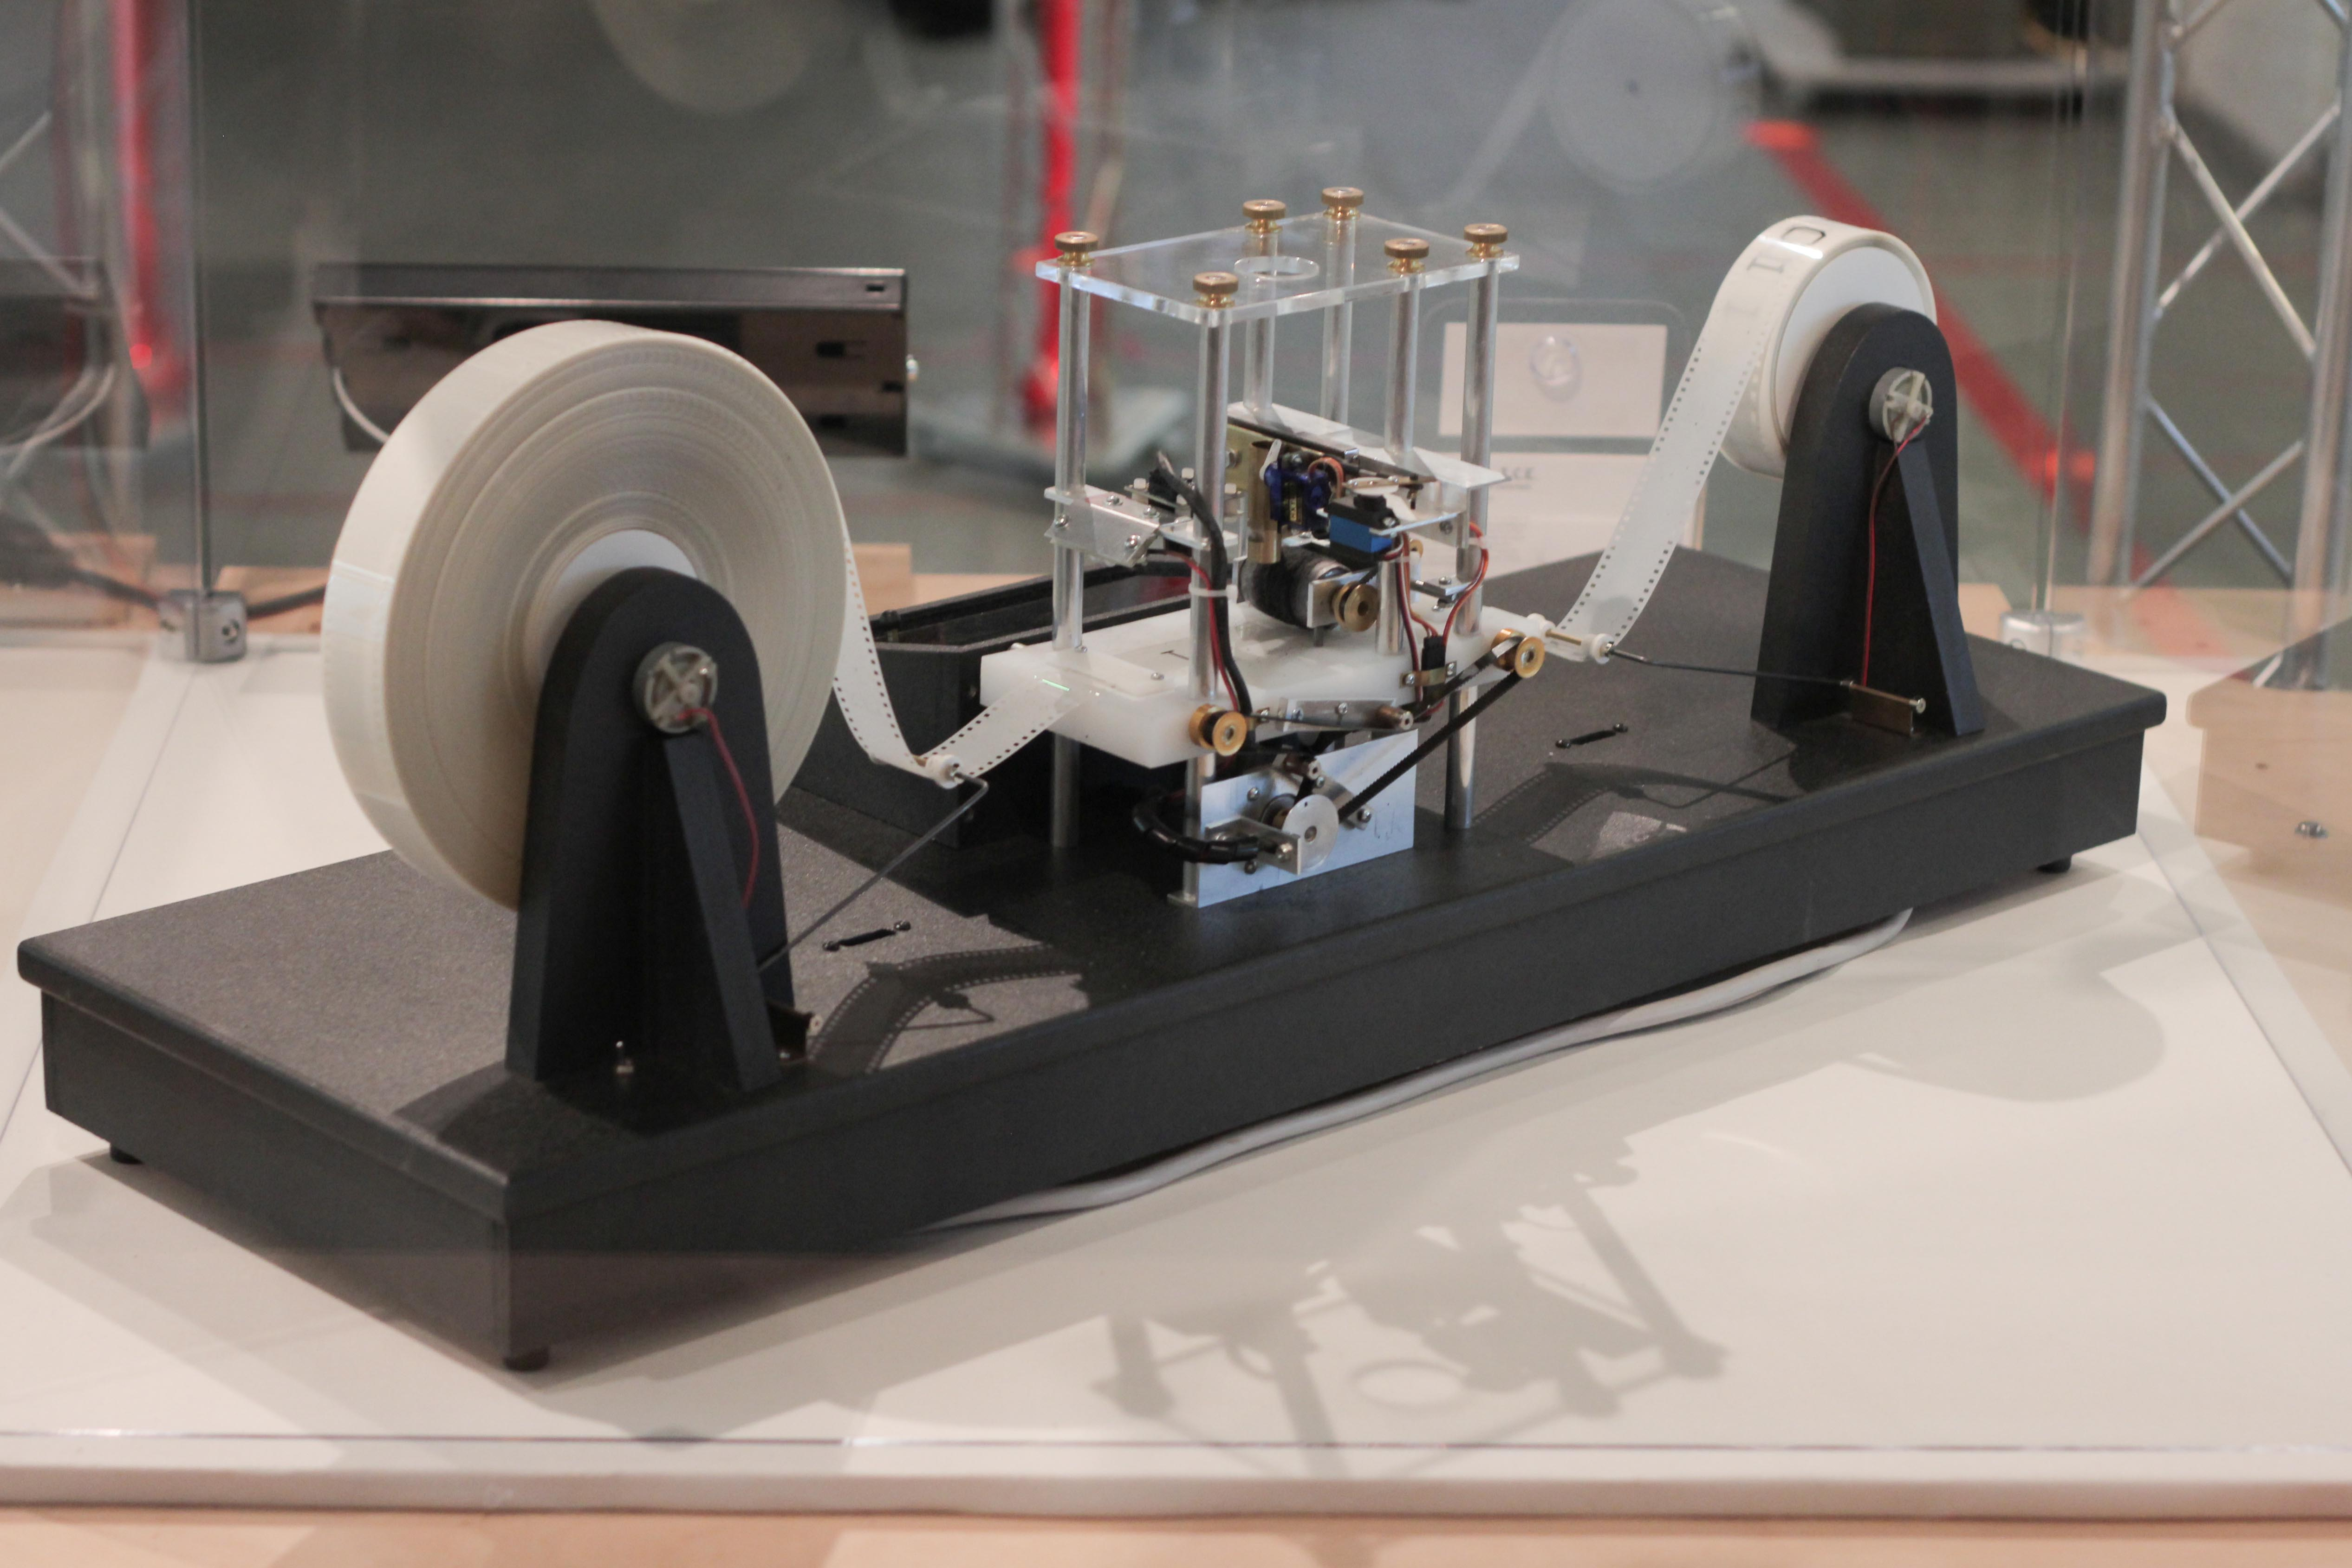
\includegraphics[width=4in]{TuringMachineDavey.jpg}
\caption{An example of a working Turing machine, constructed by Mike Davey---Copyright \textcopyright 2012 Rocky Acosta and licensed for reuse under the Created Commons Attribution License}
\end{figure}

\index{Church-Turing thesis}
\index{Turing, Alan}
The Church-Turing thesis was discovered when several finitary logic systems were developed independently, including Church's lambda calculus \citep{church1936,turing1937}.  It is hard to imagine two systems so different in approach as Church's lambda calculus and the Turing machine.  Yet, in the end, it was proven that they have the exact same computational abilities.  To be technically correct, especially with Turing machines, it is their maximum abilities which are equivalent.  A Turing machine can be defined with equivalent or less computational power than the lambda calculus, but not with more.  Thus, the computational power of finitary systems do imply a fixed set of operators.  

Such finitary systems which have this maximal computational power are known as universal machines, or universal computation systems, since they can be programmed to perform any calculation that is possible on a finitary computation system.  Thus, any computability question that would be true for one of them would be true for all of them.  Therefore, when used without qualification, incomputability usually refers to something which is incomputable on a universal computation system.

\index{Principle of Computational Equivalence}
Wolfram and van Rooij both use universal computation to set a maximal level of sophistication available in nature.  Wolfram explains his Principle of Computational Equivalence:

\begin{quote}
One might have assumed that among different processes there would be a vast range of different levels of computational sophistication.  But the remarkable assertion that the Principle of Computational Equivalence makes is that in practice this is not the case, and that instead there is essentially just one highest level of computational sophistication, and this is achieved by almost all processes that do not seem obviously simple...For the essence of this phenomenon is that it is possible to construct universal systems that can perform essentially any computation---and which must therefore all in a sense be capable of exhibiting the highest level of computational sophistication \citep[][p.~717]{wolfram2002}.
\end{quote}

\index{Tractable Cognition Thesis}
Wolfram is thus stating that within nature, computability is the limiting factor of what is possible.  Van Rooij, while restricting his comments to the nature of the mind, makes basically the same point:

\begin{quote}
Human cognitive capacities are constrained by computational tractability.  This thesis, if true, serves cognitive psychology by constraining the space of computational-level theories of cognition \citep[][p.~939]{vanrooij2008}
\end{quote}

\index{Church-Turing thesis}
In other words, if the brain is constrained by computational tractability, then it limits the possible set of models which could be used when modeling cognition.  Van Rooij specifically traces this back to the idea that the Church-Turing thesis is not merely a limitation of finitary computation, but is a limitation of reality as a whole, or, as van Rooij puts it, ``the Church-Turing Thesis is a hypothesis about the state of the world'' \citep[][p.~943]{vanrooij2008}.

Wolfram similarly applies his ideas specifically to the brain, saying:

\begin{quote}
So what about computations that we perform abstractly with computers or in our brains?  Can these perhaps be more sophisticated?  Presumably they cannot, at least if we want  actual results, and not just generalities.  For if a computation is to be carried out explicitly, then it must ultimately be implemented as a physical process, and must therefore be subject to the same limitations as any such process \citep[][p.~721]{wolfram2002}.
\end{quote}

\index{physicalism}
Thus, physicalism, when defined sufficiently to distinguish it from anything else, has been defined by its supporters as being equivalent to computationalism.  This allows a more methodical examination of physicalism and dualism to determine which is likely to be true.

\section{The Halting Problem}

\index{halting problem}
\index{programming languages!JavaScript}
One of the classic unsolvable problems in computability is the ``halting problem.''  In universal computation systems, there are ways to cause computations to repeat themselves.  However, this leads to a possible problem---if a function is poorly written, the function may get caught in a repetitive portion and not be able to leave.  This computation would be a non-halter, and therefore, left to itself, would never complete.  Most familiar computations are halting computations, as demonstrated in the following computer program. All programming examples are given in JavaScript for readability.

\begin{figure}[H]
\begin{mdframed}
\begin{verbatim}
function double(x) {
  var y;
  y = x * 2;
  return y;
}
\end{verbatim}
\end{mdframed}
\caption{A function to double a value}
\end{figure}

This program defines a function called $double$ which obviously doubles its input.  It creates a temporary variable called $y$ to hold the result of the computation and then returns $y$ as the final value for the function.  So, after defining it, the function can be used by saying $double(4)$ which would give $8$, or $double(z)$ which would take the value currently denoted by $z$ and return whatever is double of $z$.

\index{factorial function}
The next example will demonstrate the operation of a loop.  This program computes the factorial of a number which is the result of multiplying a number by all of the numbers below it down to 1.  For instance, $factorial(5)$ is $5 * 4 * 3 * 2 * 1$.  $factorial(3)$ is $3 * 2 * 1$.  So, the number of computations performed, while always finite for a finite number, varies with the value given.  A typical way to program a factorial function follows:

\begin{figure}[H]
\begin{mdframed}
\begin{verbatim}
function factorial(x) {
  var val;
  var multiplier;

  val = 1;
  multiplier = x;

  while(multiplier > 1) {
    val = val * multiplier;
    multiplier = multiplier - 1;
  }

  return val;
}
\end{verbatim}
\end{mdframed}
\caption{A function to compute the factorial of a number}
\end{figure}

This function defines two temporary variables---$val$, which holds the present state of the computation, and $multiplier$, which holds the next number that needs to be multiplied.  Unlike algebraic systems, in most computer programming languages, variables do not have static values but can change over the course of the program.  The $=$ is not an algebraic relationship, but rather it means assignment (e.g.,  $val = 1$ means that we are assigning the value $1$ to the variable $val$).  

In this program, the value of $multiplier$ is set to the number given.  Then, the computation enters the loop.  The $while$ command tells the computer that while the value in the $multiplier$ variable is greater than $1$, perform the given computation contained in the curly braces.  For example, if the function is performed with the value of $3$, $multiplier$ will start will be assigned the value $3$, which is greater than $1$.  Then the computation within the $while$ loop will be performed---it will multiply $val$ (which starts off at $1$) with $multiplier$ (which is currently $3$), and then assign that result back into $val$.  $val$ now has the number $3$.  $multiplier$ is then decreased by one, and now has the value $2$.  The bracket indicates the end of the loop computation, so the condition is re-evaluated.  $multiplier$'s value of $2$ is still greater than one, so we perform the loop again.  $val$ (which is now $3$) is multiplied by $multiplier$ (which is now $2$) and the value ($6$) is assigned back into $val$.  $multiplier$ is again decreased and is now $1$.  Now that the computation is at the end of the loop, the condition will be evaluated again, and this time $multiplier$ is no longer greater than $1$.  Because the condition is no longer true, the loop does not run again, and the computation process goes on to the next statement.  

The next statement returns the value in $val$ as the result of the entire computation.  Thus, since $val$ currently holds $6$, this function returns $6$ as the result of $factorial(3)$, which is the correct result.  Since it does eventually return a value, it is considered a halting program.  It will take longer to return a value if the input is bigger (since it has to run the loop computation process more times), and it will return invalid values if the input is less than one (or not an integer), but it will always return a value.  Therefore, since it will always complete in a finite number of steps, it is a halter.

If the programmer writing this function forgot a step, (e.g., to write the instruction that decreases $multiplier$), then instead of the previous program, the program might read as follows:

\begin{figure}[H]
\begin{mdframed}
\begin{verbatim}
function factorial(x) {
  var val;
  var multiplier;

  val = 1;
  multiplier = x;
  while(multiplier > 1) {
    val = val * multiplier;
  }

  return val;
}
\end{verbatim}
\end{mdframed}
\caption{An incorrect function to compute the factorial of a number}
\end{figure}

\index{infinite loops}
In this example, since $multiplier$ is never decreased, then, for any input greater than $1$, this function will never stop computing!  Therefore, in terms of the halting problem, it doesn't halt.

\index{universal machines}
Functions on universal computation systems are convertible to numbers.  In fact, that's how computers work---the computer stores the program as a very large number.  One example of how this can work is that each character in the above program can be converted to a fixed-size number and then joined together to a large number to denote the program.  And this is, in fact, how some programming languages work.  Most of the time, however, the conversion of a program into a number actually works by doing a more intensive conversion of the program into a numeric language that the computer understands.  

Nonetheless, in each case, the program gets converted into a (usually very large) number.  Therefore, since any program can be converted into a counting number, there are only a countably infinite number of possible programs.  But more importantly, it means that this program, since it is (or can be represented by) a number, can itself be an input to a function!

\index{decision problem}
\index{halting problem}
Some functions halt on certain inputs, but do not halt on other inputs.  The halting question can only be asked on a combination of both the program and the input since some inputs may halt and others may not.  Therefore, the halting problem is a function of two variables---the program $p$ and the input $i$.  Every program/input combination either will halt or it will not.  There is no in-between state possible on finitary computations.  Therefore, $H(p, i)$ can be denoted as a function which takes the program $p$ and input $i$ and gives as a result a $1$ if $p(i)$ halts, or a $0$ if $p(i)$ does not halt.  This is known as a ``decision problem''---a problem which takes inputs and decides if the inputs have a particular feature or match a given pattern.  Interestingly, the program $H(p, i)$ cannot be formed using a universal computation system.  This can be proved similarly to the early proof of incomputability.  

To test this, first assume that $H(p, i)$ is a program that can be implemented with a universal computation system.  If $H(p, i)$ can be implemented, then it can also be used by a longer program.  A program which does this, $N(p)$, is described below:

\begin{figure}[H]
\begin{mdframed}
\begin{verbatim}
function N(p) {
  if(H(p, p) == 1) {
    while(1 == 1) {
    }
  }

  return 1;
}
\end{verbatim}
\end{mdframed}
\caption{A theoretical function using the halting function which demonstrates its impossibility}
\end{figure}

This function starts by evaluating the halting problem of its input, $p$, given itself as the value.  If the halting problem of a program $p$ with itself as the input says ``Yes it halts'' (i.e., it gives a value of $1$), an infinite loop (i.e., a computation which does not halt) will be performed.  If not, the computation should return a value of $1$, completing the computation (i.e., the program will halt with that value).  One can ask the question, does $N(N)$ halt?  If it does, then this program will loop forever, but it can't, because we have already determined that it does not halt!  Hence a contradiction.  Likewise the reverse.  If $N(N)$ does not halt, then $N(N)$ will halt. Therefore, $H(p, i)$ cannot be solved using a universal computation system.

This process may seem like an equivocation on the nature of the functions being described
since all of the programs so far have a single input while $H(p, i)$ has two inputs.  However, any number of inputs can be encoded onto a single input using delimiters.  Therefore, specifying multiple inputs is just an easier way to write out the function than the required steps for encapsulating the inputs together into a single value.

\section[Turing Oracles as Solutions]{Turing Oracles as Solutions for Incomputable Problems}

\index{Turing Oracle|(}
\index{oracle|see{Turing Oracle}}
\index{oracle machine|see{Turing Oracle}}
\index{o-machine|see{Turing Oracle}}
Turing recognized that although the value of $H(p, i)$ was not computable, it was in fact a true function of its variables---that is, for every input set, it yielded a single output.  Thus, the halting problem was a hard problem---it had a solution, but not one that was determinable through finitary computation.  Some important questions arose from this.  Might there be other problems which are harder?  Might there be problems which require the solution to the halting problem to figure out?  If so, how does one go about reasoning about the computational difficulty of an unsolvable problem?  The answer is in Turing Oracles.

A Turing Oracle (hereafter oracle) is a black-box function (i.e. no implementation description is given) which solves an incomputable function and yields its answer in a single step.  An oracle machine is a combination of a normal computational system which also has access to an oracle.  If the oracle is well-defined in its abilities, it can be used to reason about the process even if the process as a whole is incomputable.  An oracle machine, then, is a regular machine (i.e., a normal computable function) which is connected to an oracle (i.e., the function has access to an operation which is incomputable).

Alan Turing describes the oracle machine as follows:

\begin{quote}
Let us suppose that we are supplied with some unspecified means of solving number theoretic problems; a kind of oracle as it were.  We will not go any further into the nature of this oracle than to say that it cannot be a machine.  With the help of the oracle we could form a new kind of machine (call them o-machines), having as one of its fundamental processes that of solving a given number theoretic problem. \citep[][\S{}4]{turing1939}
\end{quote}

\index{busy beaver problem}
Even though the values of functions based on oracle machines cannot be computed (since they are by definition incomputable), it is still possible to reason about which problems are reducible to oracles and which oracles they are reducible to.  Posed another way, if a programmer had an oracle for a given problem, what other problems could be solved?  For instance, there is an incomputable function called Rado's Sigma Function (affectionately known as the ``busy beaver'' function).  This function says, given $n$, what is the longest non-infinite output of any program of size $n$?  This is an incomputable function, but it can be shown to be computable given an oracle for $H(p, i)$.

\index{problem-solving}
\index{cognition}
\index{cognition!metaphysics}
If dualism is true, then at least some aspects of human cognition are not computable.  However, given the discussion above, even if human cognition is partially incomputable, cognition may be at least representable if oracles are included in the allowable set of operations.  Several researchers have previously discussed the possibility that the human mind may be an oracle machine (i.e., \citep{copeland1998}).  However, none of them have suggested including oracles as a standard part of cognitive modeling, or how one might apply oracles to cognitive modeling \citep{bartlett2010a, bartlett2010b}. The goal of this paper is to present the concept of modeling cognition via oracle machines and its application to a model of human problem-solving on insight problems.
\index{Turing Oracle|)}

\section[Partial Solutions to Incomputable Functions]{Partial Solutions to Incomputable Functions Using Additional Axioms}

\index{incomputability}
\index{axioms|(}
Incomputable functions are unpredictably sensitive to initial conditions.  In other words, there is no way to computably predict ahead of time the difference in behavior of the function from the differences in changes to the initial conditions.  If this were possible, they would by definition not be incomputable!  However, partial solutions to these functions can be made by incorporating additional axioms.

An axiom is a truth that is pre-computational.  In other words, it is a truth about computation rather than a result of computation.  Chaitin has shown that additional axioms can be used to make partial solutions of incomputable functions \citep{chaitin1982}.  For instance, if God were to say that there are 30 programs less than size $n$ that halt for a given programming language, then that fact could be used to determine exactly which of those programs were the ones that halt.  This is not a complete solution, but rather a partial solution.  Nonetheless, it is a solution larger than what was originally determinable without the additional axiom.

Now, most axioms do not come in this form, but instead state that programs that have a certain pattern of state changes will never halt.  This would not generate an exclusive list, but the list of additional programs that would be known non-halters through this axiom may be infinitely large.  Therefore, by adding axioms, one could potentially be adding infinite subsets of solutions to incomputable problems.  Axiom addition is also by definition non-algorithmic, for if axioms could be added algorithmically, then the halting problem would be solvable.  Since this is not the case, axiom addition is not an algorithmic endeavor.

Once an axiom is known, however, then the computation of halters and non-halters for which sufficient axioms are known becomes an algorithmic problem.  Therefore, the discovery of new axioms converts subsets of problems from non-algorithmic to algorithmic forms.
\index{axioms|)}

\section[Towards Defining a Turing Oracle]{Towards Defining a Turing Oracle for Modeling Human Problem-Solving on Insight Problems}

\index{problem-solving}
\index{insight problems}
\index{cognition}
The next step after investigating computability theory is to relate this theory to problems in cognitive science---namely problem-solving for insight problems.

\index{insight problems}
\index{analysis problems}
Cognitive science usually breaks problem-solving into two broad categories---analysis problems and insight problems.  Analysis problem are problems which can be solved using a known algorithm or set of known heuristics and are usually characterized by the subject being aware of how close he is to solving the problem, the benefits of continuous effort, and the use of pre-existing ideas to solve the problem.  Insight problems, on the other hand, are problems which require a reconceptualization of the process in order to solve them \citep{chronicleetal2004}. 

\index{nine-dot problem}
An example of a classic insight problem is the nine-dot problem.  In short, the problem is to take a 3x3 square of dots, and draw four lines that connect every dot without picking up the pencil.  In order to solve the puzzle, the person must realize that the solution is to extend one of the lines beyond the confines of the box, and make a ``non-dot turn.''  This reconceptualization of the problem is rare, the subject cannot gauge his or her own progress, and continuous effort is usually not as helpful as taking breaks.

\index{incomputability}
Insight problems like these have significant structural similarity with incomputable functions.  Incomputable functions can be partially solved through adding axioms to the mix.  Axioms function a bit like reconceptualizations---they allow the problem to be worked from a different angle using a different approach.  Because axioms cannot be generated algorithmically, it is difficult to conclude how close the solution is.  Likewise, because the person is not following an algorithm (which is impossible for generating an axiom), continuous effort along the same path is not likely to be helpful.

\index{problem-solving!training}
Research on the nine-dot problem has shown that training on certain ideas such as non-dot turns in similar problems produces an increased success rate in solving the problem \citep{kershawandohlsson2001, kershaw2004}.  This effectively mirrors the way axioms function in mathematical problem-solving---by increasing the number of axioms available to the subject, experimenters were able to greatly reduce the difficulty of the nine-dot problem for participants.

Because it is mathematically impossible for a person to take an algorithmic approach to the general halting problem, it cannot be classed as an analysis problem.  Because of this and its many similarities with other insight problems, the halting problem should be classified as an insight problem.  As such, the discoveries that are made for how humans solve the halting problem will help us formulate more generally a theory of human insight.

\section{Human Solutions to the Halting Problem}

As mentioned previously, if humans are able to solve incomputable functions, then the physicalism hypothesis is false.\footnote{Penrose and others have suggested that physical processes are non-computational.  However, they do so without a rigorous definition of what counts as ``physical.''  The goal is to make the definition of physical rigorous enough to be testable, and therefore have used computational tractability as the requirement.  See the section~\ref{sec:final_considerations} for additional discussion.}  The halting problem makes a good test case for this idea because it is one of the most widely studied class of incomputable problems on both a theoretical and a practical level.

Software development provides the first piece of insight into the process. In software development, humans have to develop software programs on universal computation systems, and those programs must halt.  If they do not, their programs will be broken.  Therefore, they must solve problems on at least some subset of the halting problem in order to accomplish their tasks.  In addition, the problems that they are given to solve are not of their own design, so it is not a selection bias.  It is simply not true that programmers are only choosing the programs to solve based on their intrinsic abilities to solve them because someone else (usually someone without the computational background needed to know the difference) is assigning the programs.  In addition, it is incorrect to assert that programmers are working around their inabilities to solve certain types of halting problems, because, while the programmer might add some extrinsic complexity to a program, the complexity of the problem itself has an intrinsic minimum complexity regarding a given programming language.  Likewise, simply writing it in another language doesn't help, because there exists a finite-sized transformer from any language to any other language, so being able to solve it in one language is de facto evidence of being able to solve it in another.

One may then conclude from the experience of the process of programming that significant evidence exists that humans are able to at least solve a similar problem to the halting problem.  However, there are some important caveats.

A minor caveat is that machines in real life do not exhibit true universal computation as defined in the abstract.  Universal computation systems have an infinite memory and can run forever without breaking down.  However, there are two primary reasons why this is relatively unimportant to this discussion.  The first is that even with fixed-size memory, the halting problem is still practically intractable.  That is, the reason why fixed-size memories allow the halting problem to be solved is that a programmer could do an exhaustive search of machine states to determine if the machine state contains cycles (i.e., two exactly equivalent machine states) before halting.  If so, then the program will halt.  However, calculating the result of the halting problem even using finite-sized memory would require either enormous amounts of time or memory, on the order of $2^n$, where n is the number of bits in memory.\footnote{As an example, one could solve the halting problem on fixed-size memories using a counter \citep{gurari1989}.  Since the number of possible machine states is $2^n$, then if machine states are counted, we could determine that it must be a non-halting program if the program performs more than $2^n$ computations.  A faster way of checking for cycles can be implemented, but it would generally require $2^n$ amount of memory.}  In addition, the reasoning usually given by programmers as to why something should not halt is more similar to a proof than to an exhaustive set of attempts.  If humans are regularly solving the halting problem for a large number of programs, then it is not because they are being aided by fixed-size computer memories.

The main caveat is that there exist programs (even very short programs) for which humans have not solved the halting problem.  Many open problems in number theory can be quite simply converted into a halting problem so that the answer to the problem can be solved by knowing whether or not a given computation will halt.  If humans have immediate access to a halting problem oracle, why do these programs give such trouble?

As an example, a perfect number is a number which is equal to the sum of its divisors excluding itself.  For instance, 6 is a perfect number because 1, 2, and 3 are all divisors, and they add up to 6.  It is not known if there are any odd perfect numbers.  A program could be written to search and find an odd perfect number, and halt if it finds one.  Such a program can be fairly simply expressed as:

\begin{figure}[H]
\begin{mdframed}
\begin{verbatim}
function odd_perfect_divisor_exists() {
  var i = 3;

  while(true) { // This means to loop forever unless terminated 
                // within the loop
    var divisors = all_divisors_of(i);
    var divisor_sum = sum(divisors);
    if(divisor_sum == i) {
      return i; // i.e. Halt
    } else {
      i = i + 2; // Go to the next odd number
    }
  }
}
\end{verbatim}
\end{mdframed}
\caption{A function which returns upon finding an odd perfect number}
\end{figure}

Therefore, if the above program halts, then there is an odd perfect number.  If it does not halt, then there is not one.  However, no human currently knows the answer to this question.  Therefore, whatever it is that humans are doing, it is not directly knowing the answer to the halting problem.

Will humans ever be able to solve this problem?  If humans possessed the same limitations on computation as computers, then they would never be able to solve this (and many other) problems.  However, math and science, as disciplines, assume that unknown problems with definite answers will eventually be knowable.  Simply stated, the progress of science depends on the ability of humans to eventually solve such problems as these.

In other words, if this is a fundamental limitation of humans, then the search for more and more mathematical truths may be madness---they will never be known.  This has led some theorists such as Gregory Chaitin to suppose that theorists should, in some cases, simply assume the truth or falsity of some claims as axioms, even in absence of proofs of their truth \citep{chaitin2006}.  This seems to be a dangerous road to travel.  Chaitin uses the fact that different geometries can be made from different axioms about the nature of the world to justify the arbitrariness of choosing axioms.  In the case of geometry, for instance, the two different answers to the question of whether parallel lines can intersect generates two different geometries.  However, choosing axiomatic truths for geometry is different than finding axiomatic truths for solving incomputable problems such as the halting problem, because in the former the axiom is unconstrained within the system and in the latter it is constrained but unprovable within the system.  If an axiom is unconstrained, then given the remaining axioms, a fully consistent system can be maintained with either choice of axiom.  In other words, either axiom is equally consistent with the remaining axioms.  If an axiom is constrained but unprovable, then the truthfulness of an axiom is dependent on the remaining axioms.  In other words, one axiom is true and another is false given the remaining axioms.  In the case of reasoning about the halting problem, programmers are dealing entirely with constrained but unprovable axioms.  It might be a worthwhile endeavor to provisionally accept an axiom and see where it leads, but it is dangerous to include a provisionally accepted axiom on equal ground with other types of axioms in formal mathematics.

Another option, however, is that humans are able to incrementally arrive at solutions to halting problems.  This would mean that humans have access to an oracle which is more powerful than finitary computational systems, but less powerful than a halting oracle.

\section{An Oracle for Insight Problems}
\index{hyper-computation}
Selmer Bringsjord has argued for the mind being hyper-computational on the basis of his research into human ability to solve the halting problem.  His group claims that they could always determine the halting problem for Turing machines of size $n$ if they took into account the determination of the halting problem for Turing machines of size $n - 1$ \citecustom{bringsjord2006}{Bringsjord, Kellet, Shilliday, and Taylor}.

Bringsjord's group has quite a bit of experience with the halting problem, but it is impossible to tell if his formulation is completely true based on the size of the problem space when $n$ goes beyond 4---there are then too many programs for humans to analyze (when $n$ is 5 there are 63,403,380,965,376 programs).  What he found, though, is that his group could formulate halting proofs for programs of size $n$ based on previous patterns which were identified for size $n - 1$.  They used the proofs that they made for size $n - 1$ as a basis for the proofs in programs of size $n$.  This is itself an interesting result, though it is hard to say that these are necessarily based on program size, since there is nothing in the halting problem that is program-size dependent.  A better interpretation is that the proofs were built by introducing constrained axioms.  The larger programs utilized the axioms introduced in smaller programs, but potentially required more axioms to solve.  Therefore, the proofs utilized the smaller programs because they utilized the axioms demonstrated there.  As the programs became larger, the number of axioms required to determine a solution also grew.

This explanation actually fits surprisingly well---it is non-algorithmic (it is determining unprovable axioms), it is incremental (each axiom gives more explanatory power), and it is weaker than a halting oracle.

To put this more formally, let's define some values: 

\begin{description}
\item{$A$}
the minimum set of axioms required to solve $Q(p, i)$

\item{$Q$}
a decision problem (such as the halting problem)

\item{$p$}
a program

\item{$i$} 
the input to program $p$

\item{$B$}
a set of axioms such that the size of the set of the intersection of $A$ and $B$ is one smaller than $A$.  In other words, $B$ contains all of the axioms required to solve $Q(p, i)$ except one.
\end{description}

From these definitions human insight can be described by the following oracle:

\begin{equation}
A = I(Q, p, i, B)
\end{equation}

\index{axioms}
In other words, if a human is given a decision problem over a certain input, and he or she knows all of the axioms needed to solve the problem except one, then human insight will reveal the remaining axiom.  If true, this would explain why insight is both incremental and non-computational.  It goes beyond what is available to computation, but still has prerequisites. In this proposal, all axioms are known except one.  Thus, in the case of finding odd perfect numbers, the problem of finding the solution to the problem is that there are not enough pre-existing axioms to infer the final axiom.

\section{Problems and Directions}

The main problem with the description as stated is that there are different kinds of axioms, yet there is insufficient mathematical theory (at least known to the author) to differentiate types of axioms.  At present, a distinction should be made between bottom-up and top-down axioms.  As mentioned earlier, if God would say that there are $x$ halting programs of size $n$, a programmer could determine which ones they were by running all of them simultaneously until $x$ of them halt.  This kind of axiom, a ``top-down'' axiom, requires prior knowledge of the entire spectrum of the problem to determine.  Another kind of axiom, a ``bottom-up'' axiom, requires a minimum of understanding in order to be apprehended. Its truth is knowable even if not provable within its own formalism, and its application is not intrinsically bounded.  

\index{analysis problems}
\index{insight problems}
\index{logic!second order}
\index{logic!first order}
An example of a bottom-up axiom is an axiom which says that if a program has a loop whose control variable is monotonically decreasing and has a termination condition which is greater than its start value then that program will never halt.  That axiom, which is provable by induction, will then allow a programmer to determine the value of the halting problem for an infinite subset of programs.\footnote{Some may claim that, since it is proved using an inductive proof, this statement becomes a theorem rather than an axiom.  However, it is only a theorem from second-order logic, since general induction requires second-order logic and can only be imported to first-order logic as an axiom \citep{enderton2012}.  Since the machine itself is a first-order logic machine \citep{turing1936}, it is an axiom from the perspective of the first-order system.}  Thus, it acts as a bottom-up axiom.  In addition, as should be obvious, the introduction of such an axiom converts an infinite subset of problems from insight problems to analysis problems.  Knowing such axioms allows the programmer to proceed algorithmically!

As a result, several open questions emerge:

\begin{enumerate}
\item Are there other properties of axioms which are important to the sequence in which they may be found?
\item Are there other prerequisites for finding these axioms?
\item In what ways (if any) do axioms relate to program size?
\item Is there a proper way to measure the size of an axiom?
\end{enumerate}

\index{Omega}
\index{OmegaSymbol@$\Omega$|see{Omega}}
Chaitin's proposal for measuring axioms is related to his $\Omega$ probability.  $\Omega$ is the probability for a given Turing machine as to whether or not it will halt, which, for the sake of his theory, is written out as a string of bits.  Chaitin measures axioms by the number of bits of $\Omega$ they are able to compute.  If an axiom can deduce two bits of $\Omega$, then the axiom is two bits long \citep{chaitin2007}.  A naive approach to using this definition might say that humans are able to deduce a single bit of $\Omega$ when needed.  However, these bits are much ``smaller'' than the types of axioms that humans tend to develop, which are much wider in extent, as each bit of $\Omega$ is a single program, rather than a collection of programs. There seems to be, based on experience, some intrinsic ordering on the discoverability of axioms present within $\Omega$.  An algorithm can discover 1s (halts) within omega, with an implicit ordering based on length of program and the program's running time.  For instance, a program could be written which started program 1 at time 1, program 2 at time 2, etc.  Each iteration would run one cycle of each current program and start one new program.  Each program that halts gives one bit of omega.  Therefore, by exhaustive search, solutions to $\Omega$ can be discovered one bit at a time.  However, this does not match the way humans arrive at the solution, which is a more generalized axiomatic approach (covering multiple cases of programs at a time---not just a single instance like $\Omega$).  Likewise, such algorithms can never discover the 0s (non-halters).   Therefore, although $\Omega$ is a powerful conceptualization of the solution to the halting problem, it is unlikely to be helpful in the types of axioms that humans appear to be discovering.

\index{axioms}
Another possible way to measure the size of an axiom is to measure the size of the recognizer function needed to recognize instances of the axiom.  But again, it is unclear whether or not that would be the measurement which would give us the proper ordering of axiom determination.  It may be harder to implement a recognizer than it is to intuitively recognize an axiom. 

Therefore, in order to proceed further, additional research is needed into the nature of axioms themselves, and different ways that they can be categorized and quantified in order to find a natural sizing and ordering for them.


Again, two questions emerge that relate to the embodiment of the oracle itself:

\begin{enumerate}
\item How reliable is the axiom-finding oracle?
\item What are individual differences in this oracle?
\end{enumerate}

The answers to such questions will lead to more understanding about how the oracle interacts with the rest of the mind's systems.

\section{Generalizing the Oracle Method}

\index{Turing Oracle}
\index{cognition!metaphysics!physicalism}
Although important, the main focus of this paper is not the specific oracle outlined above.  The larger point is that if an operation in the mind is non-physical, this does not preclude it from being modeled.  Specifically, oracles seem to fit the bill for a wide variety of non-physical operations.  There are probably other operations which will require other formalisms, but formalisms should not be avoided simply because the formalism is not physically computable.  

So how does one make a general application of oracles to modeling the mind?  First of all, it is important that the operation under consideration be well-defined in terms of what it is doing.  It is not worthwhile to simply state ``something occurs here''---such is not a well-specified description.  In the example above, specific preconditions (a decision problem, a program, its input, and a set of existing axioms) and a specific postcondition (the needed axiom to solve the problem) have been postulated.  William Dembski's concept of specification could be used to determine whether or not the given specification is too broad or if it is reasonably constraining.  Dembski's measurement is basically a relationship of the potentially described target states to the specification length.  If a specification doesn't sufficiently limit the target space of possibilities, it is not a useful specification \citep{dembski2005}.  

Second, specific reasons must exist in order to believe that the proposed process is incomputable.  Since solving the halting problem is known to be incomputable, and adding axioms is incomputable by definition (otherwise they would be theorems), then specific evidence indicates that the proposed process is incomputable.  

\index{testability}
The hard part then comes in testing the theory.  Because the results are incomputable, and not even likely reducible to a probability distribution, testing it is more difficult.  In the case of computable causes, a specific end-point prediction can be established by computation, and then the result can be validated against that computation.  In this case, the result is not computable, and therefore validation is more difficult.  Validation will often be based on the qualitative description of the process rather than a quantitative prediction.  Parts of it may still be quantifiable, but only with difficulty.  For instance, to test the example presented, a method of identifying and counting the number of axioms within a person's mind is needed in order to come up with a quantifiable prediction.  However, since this is not possible, it can only be tested based on secondary quantifications.  Thus, testability on proposed oracles becomes much more dialectic.

\section{Applications}

\index{traveling salesman problem}
This method of using oracles for modeling human cognition has many applications to both psychology and engineering, as well as to the history of technology.  For psychology, it introduces a new way of evaluating mental causes, and a new formalism for modeling and testing them.  In several known cases, human problem solving outperforms what is expected from computationalism.  For example, one group of researchers
reported that human performance on the Traveling Salesman Problem scales linearly with the number of nodes, which far surpasses any computational estimator for the problem \citecustom{dryetal2006}{Dry, Lee, Vickers, and Hughes}.  Therefore, modeling human performance in terms of an oracle machine may allow more accurate predictions of performance.

\index{complexity!metrics}
For engineering, oracles can be used to better identify and measure complexity.  If axioms become quantifiable, and the number of axioms required to solve problems becomes quantifiable, then this can transform the practice of complexity estimation.  One such method to use these ideas to calculate software complexity is given in \citet{bartlett2012}.  

\index{software development}
\index{software game development}
This idea can also be applied to software computer games.  Many computer games are organized by ``levels'' so that each level is harder than the previous one.  One could use axioms as a measure of hardness, and construct the levels so that each one introduces a new axiom used to complete the game.  This would allow a more rigorous approach to game level design at least in certain types of computer games.

\index{technological history}
\index{independent discovery}
A final way of using this idea is in understanding the history of technology, including science and mathematics.  It has been a curious feature that many ``leaps'' in scientific or mathematical thought have been made simultaneously by multiple people.  Isaac Newton and Gottfried Leibniz both independently invented calculus, Gregory Chaitin and Andrey Kolmogorov both independently invented algorithmic information theory, Elisha Gray and Alexander Graham Bell both filed a patent for the telephone on the same day, and the list goes on and on \citecustom{aboitesetal2012}{Aboites, Boltyanskii, and Wilson}.\footnote{Appendix A of \citet{aboitesetal2012} contains quite an impressive list of codiscoveries.}  This model, if correct, would validate the view of T. D. Stokes that ``even though there is no algorithm of discovery, there are logical elements present in the process whereby a novel hypothesis is devised\ldots{}'' \citep[][p.~111]{stokes1986}.  This model presents a non-algorithmic process and shows the logical elements which are within its prerequisites.  Therefore, when ideas are widespread, multiple people will each be a single axiom away from discovery.  Consequently, faced with the same problem, many different people will be able to realize the same missing axiom.

\section{Final Considerations}
\label{sec:final_considerations}

\index{cognition!metaphysics}
\index{cognition!metaphysics!physicalism}
\index{cognition!metaphysics!dualism}
There is good evidence human cognition goes beyond what has been traditionally considered as ``physical,'' and a lack of physicality does not preclude cognitive modeling.  ``Physical'' has been defined as ``computable'' in order to avoid the ambiguities of the term.  This is important because someone might try to assert that humans have a separate soul and that it is simply physical.  Without a solid definition of what is and is not physical, nothing prevents such a formulation.   

\index{Turing Oracle}
\index{consciousness}
Roger Penrose and Jack Copeland have both made a similar suggestion \citep{copeland1998, hodges2000}.  Both have agreed that humans seem to be oracle machines, but in a purely physical sense.  However, neither of them provided a sufficient definition of what counted as physical or non-physical to make a proper distinction.  Nothing that either of them has said would contradict what is defended in this paper, though Penrose argues that there is even more to human consciousness than is representable through oracle machines---a position also not in contradiction to the claims defended here.   For instance, it is hard to consider the act of true understanding as a process involving numbers at all, as John Searle's Chinese Room argument shows \citep{searle1980}.

\index{idealism}
Another possible objection, then, is to say that the universe as a whole isn't physical.  It could be possible, for instance, that even the fundamental laws of matter are only fully describable using oracles, and none of them at all are computable with finitary methods, and therefore finitary methods can only be used to solve certain macro-systems which are the exception rather than the rule.  However, even if true, that would not lead to the conclusion that physicalism is true and incomputable functions should be classified as physical along with computable ones.  Instead it would reveal that the idealists such as Richard Conn Henry \citeyearpar{henry2005}, who believe that the physical is a mere epiphenomenon and the non-physical is what is really real, were the ones who were right all along.  Douglas Robertson \citeyearpar{robertson1999} comments:

\begin{quote}
The possibility that phenomena exist that cannot be modeled with mathematics may throw an interesting light on Weinberg's famous comment: ``The more the universe seems comprehensible, the more it seems pointless.'' It might turn out that only that portion of the universe that happens to be comprehensible is also pointless.
\end{quote}

In any case, while it is certainly an improbable proposition, it is a logical possibility that physicalism is not true even for physics!  

\index{insight problems!animals}
While the present discussion focuses on models of \textit{human} insight, that limitation is purely practical---there is no known way of detecting or measuring insight behavior on non-human creatures---and there is no philosophical, theoretical, or theological reason why such processes could not be occurring in other creatures at a much lower level.  Nothing in this proposal limits itself either to modeling humans or even organisms.  However, in humans it seems most obvious and evident that restricting reality to only computable functions is incorrect.

\eandmbibliography{Bartlett1Library}

\chapter{Calculating Software Complexity Using the Halting Problem}
\author{Jonathan Bartlett}

\begin{abstract}
Calculating the complexity of software projects is important to software engineering as it helps in estimating the likely locations of bugs as well as the amount of resources required to modify certain program areas.  Cyclomatic complexity is one of the primary estimators of software complexity which operates by counted branch points in software code.  However, cyclomatic complexity assumes that all branch points are equally complex.  Some types of branch points require more creativity and foresight to understand and program correctly than others.  Specifically, when knowledge of the behavior of a loop or recursion requires solving a problem similar to the halting problem, that loop has intrinsically more complexity than other types of loops or conditions.  Halting-problem-like problems can be detected by looking for loops whose termination conditions are not intrinsically bound in the looping construct.  These types of loops are counted to find the program complexity.  This metric is orthogonal to cyclomatic complexity (which remains useful) rather than as a substitute for it.
\end{abstract}

\section{Complexity Metrics in Software}

Managing software development is often about managing risks - knowing which tasks are likely to take more time than others, which features are more likely to impact others, how much testing will be required to make sure that a feature is solid, and whether a bug fix or a feature implementation requested right before release will be more likely to make the code more stable or lead to other bugs.

One of the key considerations of risk management is software complexity.  Complex software is inherently more difficult to build, test, and maintain.  Therefore, it is critical for software development managers to know which parts of code are most complex and therefore more likely to incur failures if modified.

\section{A Brief History of Software Complexity Metrics}

Early complexity metrics were based almost entirely on the amount of code produced.  Therefore, a function which contained 10 lines of code was considered more complex than one which contained only 5.  However, since ``lines'' of code is often includes stylistic approaches, Halstead developed a set of measures based on the number of operators and operands present within the code.\cite{kearney}  

Lines of code and related metrics are still often used for software effort estimation, but its use in analyzing code complexity has fallen away.  It quickly became clear that not all code is the same, and some operators are inherently more complex than others.  Specifically, the decision structure of the program was inherently more complex than the computations.  Cyclomatic complexity was created to measure the size of the decision structure of the program.\cite{mccabe}  This is done by creating a graph of all basic code blocks as nodes, and then edges which show how control can move between them.  The formula for calculating the complexity is:

$$E - N + T$$

$E$ is the number of edges, $N$ is the number of nodes, and $T$ is the number of terminating nodes (entry and exit points - usually 2).   

Cyclomatic complexity is extremely useful in determining how to test software.  The cyclomatic complexity of a program is also the minimum number of tests needed to cover every control flow branch of a program.  If the cyclomatic complexity of a program is 5, then at least 5 tests must be devised to test every branch of code.  Such tests do not guarantee total coverage of all possible test conditions, but they will verify that every statement in the program will contribute to at least one test.

The ABC metric is a simplified metric combining aspects of both lines of code and cyclomatic complexity.  It works by simply counting the number of assignment statements, the number of branches (direct flow control shifts - i.e. function calls), and the number of conditionals.\cite[pg.~2--3]{fitzpatrick}  These can then be analyzed on a whole program, per-module, or per-function basis, to give an overview of complexity and size of a software program.

\section{Deeper Difficulties in Software}

While each of the previously-mentioned metrics have their usefulness, none of them get at the deeper difficulties that make software projects complex.  Many programming languages have attempted to remove the inherent difficulties within software.  Some, like COBOL, attempted to remove the mathematical notation common to programming languages.  Others, like Java, attempt to simplify software by encapsulating related methods into objects.  Visual programming languages, such as Flowcode, turn all software into visual representations, allowing the user to drag and drop flowchart-like components to accomplish programming tasks.  The idea is that it is the text-based nature of the software which causes complexity and confusion within software.

While each of these actually do relieve certain specific problems in software development, none of them are able to remove the complexity of software development, because the complexity is inherent in the nature of software development itself.  What makes software difficult is their open-ended nature.  Most general-purpose programming languages today are Universal in nature - that is, they can perform any computable function that any other programming language can perform.  Thus, they are open-ended - the types of operations that they perform are entirely specifiable by the programmer, and are not restricted.

Universal programming languages are chaotic - that is, there is no easy mapping between programs, data, and results.  Therefore, predicting the output over a wide swath of code and data can be difficult.  

So what parts of a language cause a language to be chaotic?  Arbitrary looping structures.  Interestingly, this is precisely the same part that causes it to be open-ended.  Arbitrary looping structures allow a programmer to generate any possible computable function.  As such, they also allow a programmer to write programs whose results are chaotic.  In practical terms, arbitrary looping structures are \verb+while+ statements, \verb+jump+/\verb+goto+ statements, recursive functions, and continuations, though others may be possible.

Occasionally, the solution to this problem has been to reduce the scope of the language.  SuperGlue is one language which is specifically designed to be as expressive as possible while avoiding constructs that lead to complexity.\cite{mcdirmid}  However, ultimately, to get beyond the originally conceived computational bounds of the programming language, Universality, as well as the complexity that goes with it, are required.

\section{The Halting Problem as an Insight Problem}

As discussed elsewhere in this volume, some problems are not amenable to analytical analysis, and require insight in order to solve them.\cite{bartlett1}\cite{holloway}  Neither are such problems computable - no computer is capable of calculating these problems.  One such problem that is relevant for us is the halting problem.

The halting problem states that, given a Universal language, there is no program that can be written which will tell if any arbitrary program written in that language will ever complete (i.e. halt).  This is not based on the size of the program code, but rather of the nature of the constructs available.  This is not to say that one couldn’t write a program to tell if certain subsets of programs written in that language will halt, but there could not be a program to tell if any given program would halt.

The interesting thing about this, as noted by Bartlett\cite{bartlett1}, is that computer programmers seem to be able to possess this power to some degree.  Since the complexity of problems assigned to them are arbitrarily hard (i.e. management, not the programmer, often decides what must be done), and the reason that arbitrarily hard programs are possible is because of the open-ended nature of Universal programming languages (the parts of the language which *create* the chaos are precisely the ones *required* for programs of arbitrary complexity), we can say that human programmers are generally reliable halting problem solvers.

There are cases (usually coming from number theory) where programs (even very simple ones!) are not known whether or not they halt.  These are interesting, and it certainly seems that there are different levels of hardness and different levels of insight required to make determinations.  Nonetheless, the advancement of science and mathematics actually depends on the ability of humans to be able to accomplish this.  In other words, if we doubt the ability of humans to figure out such problems, then we should cast doubt on the progress of science itself.  Should we tell mathematicians to stop looking for answers in number theory?   Or should we assume that the insight will come one day?  I argue that the ability of programmers to reliably solve halting problems in their daily work should lend hope to the mathematicians that someone will be able to have the insight to solve their problems as well.

\section{Using the Halting Problem to Measure Software Complexity}

The trouble with insight problems is that they are not reliably solved by individuals.  They are unreliably solvable - in other words, we can trust that a solution is possible, but we can’t rely on an analytic procedure to do so.  Even worse, if a programmer doesn’t realize that they are looking at an insight problem, they might not know that special care must be taken.

So how can we recognize an insight problem in code?  Since we have already determined the types of programming structures which make a program universal (arbitrary looping structures), we can therefore detect those structures in code.

For most programming languages, the main structures which must be detected are:

\begin{enumerate}
\item Loops where the iterations are not implicit in the control structure
\item Recursive functions (which are just another way of implementing \#1)
\end{enumerate}

For \#1, consider the following two programs that each print out the square of every number in an array:

\begin{figure}[H]
\begin{verbatim}
ary.each{|x| puts x * x}
\end{verbatim}
\caption{A program with an implicitly-terminating loop}
\label{fig:impterm}
\end{figure}

\begin{figure}[H]
\begin{verbatim}
i = 0
while(i < a.length) {
	puts x * x
	i = i + 1
}
\end{verbatim}
\caption{A program with an arbitrary looping structure}
\label{fig:expterm}
\end{figure}

The implementation in Figure \ref{fig:expterm} is more complex than the one in Figure \ref{fig:impterm}, but not because of the size of the program.  What makes it more complex is that it utilizes an arbitrary looping structure - the while statement.  In Figure \ref{fig:impterm}, the looping in inherently bound by the loop operator.  In Figure \ref{fig:expterm}, the programmer must specifically act to make the loop terminate appropriately.  There is no way an \verb+each+ statement on its own will fail to halt.  There are many ways in which a while statement can fail to halt.  The termination is decoupled from the loop construct itself.

Therefore, as a first pass to measure software complexity, we will simply count the number of open-ended looping structures (either as loops or recursive functions) which occur in the program.   

\section{Adding Axioms to Minimize Insight}

However, as is obvious from the simple example above, there are many well-understood conventions which mitigate the complexity of certain kinds of open-ended looping structures.  In the example above, starting at zero, monotonically increasing, and then terminating at a predetermined stopping point, while it may not be codified within the language, is a well-understood looping convention that, if followed correctly, will result in the loop’s termination.

Chaitin formalized this idea in his algorithmic information theory.  He pointed out that while certain problems were unsolvable given a base set of axioms, by incorporating additional axioms into the problem, solutions can be found.  For instance, following Chaitin, if God were to tell us how many programs of size N halted, we could use that information to solve the halting problem for programs of size N.\cite{chaitin}\footnote{For a proof of this, consider that the issue that makes the halting problem difficult is that if you follow the execution of the program, the ones which don’t halt will never finish, but we won’t ever \emph{know} that it will never finish, since at any moment it may still finish.  However, if we know that X programs of size N will halt, you can simply run all programs of size N simultaneously.  Then, we can wait until those X programs finish, and we will know that the rest of the programs will never finish.  Therefore, we know that we can know the answer to all the halting problems in a finite length of time - the length of time will be the maximum runtime of the longest-running halting program.}

In the same way, when a convention for constraining repetition is discovered, it can be incorporated into a canon of axioms which are also known to halt.  And thus it should be treated almost on the same level as a language construct which produces close-ended loops.  I say ``almost'' because language constructs enforce the validity of the axiom by force, while conventions require that the programmer follow the convention correctly.

This cannon of axioms can be codified into an extensible static analysis tool to check program complexity.  Such a tool could consist of the set of potential non-terminating constructs, as well as a ``book of conventions'' which are the known conventions for ensuring termination.  The tool would then measure the potential number of non-terminating constructs which do not conform to a pattern in the ``book of conventions.''\footnote{A similar procedure was independently developed by Bringsjord et al\cite{bringsjord}, Hertel\cite{hertel}, and Harland\cite{harland}, though differing in many aspects and applications.  Their solutions were to categorize non-halters rather than halters, and to do it based on runtime patterns rather than a static analysis of structural patterns in the program.  They identified well-known patterns, data-mined for others, and then used a symbolic induction prover to match potential programs with these patterns. In addition, their purpose was for answering questions about computer science theory (specifically, the busy beaver problem) rather than assessing program complexity.}

In addition to the constructs which can be statically analyzed, some conventions (often termed as ``patterns'') will not be easily amenable to inference by software.  They should, however, at least be documented, and they can be manually marked or removed after-the-fact.  However, if the construct is not amenable to static analysis, extra effort should be taken to review all implementations of the construct manually.

It should also be recognized that these axioms should be treated as first-class insights.  That is, the ``book of conventions'' should be considered a set of valuable intellectual assets.  As solutions to insight problems, the ``book of conventions'' is by definition a set of solutions which are not immediately obvious, and, therefore, if a convention is not recorded, and is therefore ``lost'', it could well be a permanent loss of insight for an organization.

\section{Using the Metric}

The ultimate goal of the metric is to reduce the complexity of the software to zero.  Remember, when a pattern which solves a restricted subset of the halting problem is discovered, it can be incorporated as a new axiom into the ``book of conventions''.  Therefore, if there are any areas in the program which are marked as being complex, that means that it is still not known if the program will even finish!  If a developer has a new insight into why a certain section of code will finish, this should be documented in the ``book of conventions''.  If the programmer cannot state why they think that the program will finish, it should be reviewed or rewritten.  If the code cannot be reworked, and the program cannot be proven to terminate, it should be considered highly suspicious.

In addition, areas of code which are complex given the constructs, but found in the ``book of conventions'' should be flagged for a second-pass review, to make sure the conventions were followed appropriately.  Also, those sections should also be flagged for programmers making modifications, to be sure that their modifications do not upset the assumptions of the conventions.

\section{Further Considerations}

While this metric is very useful, it is obviously not the last word on complexity metrics.  It does not technically supersede the other complexity metrics mentioned.  Lines of code is still a useful planning tool.  Cyclomatic complexity is still a useful test coverage tool.  However, this metric can be useful in identifying programming patterns which are intrinsically problematic, and help mitigate possible problems with documentation, code review, and testing.  

For future development, similar ideas could be applied not just to the halting complexity, but also to the complexity that variables are derived from.  When the value of a variable is determined by multiple loops, or conditions within loops, or other sorts of non-linear mechanisms, the value of variables can be chaotic, even when they are not themselves what determines if the problem halts.  Extending these ideas to variable calculation could allow for an even more comprehensive look at where program complexity lies.

\bibliographystyle{plain}
\bibliography{Bartlett2Library}




%% \documentclass[cmfonts]{witpress}
%% \usepackage{algorithmic}
%% \usepackage{algorithmextra}
%% \usepackage{lscape}
%% \usepackage{graphicx}
%% \usepackage{psfrag}
%% \usepackage{amsmath}
%% \usepackage{amsfonts}
%% \usepackage{amsthm}
%% \usepackage{cite}
%% \usepackage{makeidx}
%% \usepackage{longtable}
%% \usepackage{amssymb}
%% \usepackage{balance}
%% \usepackage[lastname]{authorindex}
%% \usepackage{subfigure}
%% \usepackage{listings}
%% \usepackage{color}
%% \usepackage{rotating}
% declare the path(s) where your graphic files are
%% \graphicspath{{./}}
%% \DeclareGraphicsExtensions{.eps,.png}

\eandmchapter{CSI Collecting}{Complex Specified Information (CSI) Collecting}{Eric Holloway}{Independent Scholar}

\begin{abstract}
Intelligent Design Theory makes use of the concept of intelligent agency as a distinct causal mode, distinct from chance or algorithmic modes of causation.  The influence of such agency is often detected by the contribution of information to a search process.  Assuming humans are capable of such causal roles, then it should be possible to measure the amount of information that a human is contributing to such a process.  This is done by measuring the success rate for a search for a solution to a computationally hard problem by both humans and computers.  The methodology used for this experiment was not successful, but it is hoped that the experimental setup and methodology will inspire further improvement and research in this area.
\end{abstract}

\section{Introduction}
Research comparing human cognitive capabilities to computer algorithms suggest humans possess \index{supra-computational cognition}supra-computational cognition.  Humans are capable of finding good solutions to computationally intractable problems, and this capability scales at a faster rate with larger problems than the best known algorithms \citecustom{dry06:_human_perfor_visual_presen_travel}{Dry, Lee, Vickers, and Hughes}.  Many popular games are algorithmically intractable to solve \citep{viglietta11:_gamin_is_hard_job_but}.  Programmers appear capable of solving halting problems \citep{bartlett11:_calcul_softw_compl_using_haltin_probl}.  People can solve insight problems, for which there is currently no known computational method \citep{bartlett11:_using_turin_oracl_in_cognit_model}.  Observers can pick out targets in a picture relevant to their goal independently of the target's features \citecustom{gue12:_featur_indep_neural_codin_of}{Gue, Preston, Das, Giesbrecht, and Eckstein}.  Such capabilities either have never been algorithmically emulated, or violate well known and well substantiated computational constraints, such as the computational complexity of the problem \citecustom{cormen01:_introd_to_algor}{Cormen, Leiserson, Rivest, and Stein}, the \index{No Free Lunch Theorem (NFLT)}No Free Lunch Theorem (NFLT) \citep{wolpert96:_no_free_lunch_theor_for_optim,wolpert95:_no_free_lunch_theor_for_searc} and the halting problem \citep{cover06:_elemen_of_infor_theor}. 

\index{Intelligent Design Theory (IDT)}Intelligent Design Theory (IDT) provides a formal language to account for observations of supra-computational cognition.  According to IDT, intelligent agents, such as humans, are capable of creating a new form of information called \index{complex specified information (CSI)}complex specified information (CSI) \citep{dembski:_specif}. Dembski's work on \index{search algorithms}search algorithms \citep{dembski06:_conser_of_infor_in_searc} implies that if human interaction can be incorporated into a search and \index{optimization}optimization algorithm, these algorithms can surpass the limitations of the NFLT  over a wide variety of hard problems.  This is possible due to the unique ability of \index{intelligent agents}intelligent agents, such as humans, to create CSI.  A further implication is the user does not need specialized interfaces or training for each type of problem.  The possibility of such a \index{generalized interface}generalized interface is suggested by research demonstrating \index{context independent problem solving}context independent problem solving by humans \citecustom{sperber95:_relev_theor_explain_selec_task}{Sperber, Cara, and Girotto}, and suggested by IDT's implications.

\section{Problem Description}

In the computational domain, it is problematic to identify whether human interactions can be defined by an algorithm.  Since all the interactions with the computer are defined by a series of 1s and 0s, i.e., a \index{bit string}bit string, the interaction can be codified by an algorithm that outputs the same bit string.  Consequently, on first analysis, trying to computationally distinguish human interaction from algorithm output seems impossible.  If human interaction is indistinguishable from algorithmic output, then it is not plausible human interaction can surpass the No Free Lunch Theorem (NFLT).  Such is the basic problem addressed: How is it possible to \index{distinguish human interaction}distinguish human interaction from algorithm output?

Even though it is always possible to codify a series of events in a finite domain after the fact, the question is whether such codification is possible prior to the event's occurrence.  A prior codification is not possible in all cases; otherwise, it violates the \index{halting problem}halting problem \citep{cover06:_elemen_of_infor_theor}.  This means the possibility of codifying a human's interaction after the interaction has occurred does not necessarily entail it can be codified before the interaction.  Consequently, it is possible that with the right experimental design a human's interaction can be distinguished from an algorithm output.

\section{Background}\label{sec:background}

The question is, what is the experimental design that can make the distinction between human and algorithm?  One approach is to use the NFLT.  The theorem sets precise, rigorous boundaries on the \index{mathematical capabilities}mathematical capabilities of algorithms. Anything performing outside of these boundaries is by logical necessity \index{non-algorithmic}non-algorithmic.  To show \index{humans are supra-computational}humans are supra-computational, one need simply show they do not abide by the NFLT.  Unfortunately, such a demonstration may be impossible.  The NFLT only applies across all problems within a very small, specialized subset of problem types.  As such, the NFLT is quite difficult to apply in practice.

The \index{Almost No Free Lunch Theorem (ANFLT)}Almost No Free Lunch Theorem (ANFLT) \citecustom{droste02:_optim_with_random_searc_heuris}{Droste, Jensen, and Wegener} provides a solution.   The theorem shows while the original NFLT does not apply to most particular problem domains, the expected performance for most algorithms on many real world problems does not vary significantly between algorithms.  There is almost no free lunch for a large portion of \index{real world problems}real world problems. 

The ANFLT result implies that given a search algorithm, as long as the algorithm is selected independently of the problem, it is unlikely the choice of algorithm  makes a significant difference in search performance.  Consequently, if \index{human interaction capability} human interaction discovers a solution significantly better than search algorithms, it is very likely the interaction was non-algorithmic, and therefore supra-computational.\footnote{Throughout this paper, the term \index{solution}``solution'' refers to both the best/true solution to a problem, as well as substandard solutions to a problem.  Even in the case where there is only one true answer to a problem, there may be other answers that are approximations of the true answer.  The two types of solutions are distinguished in terms of their optimality.  The true solution is the \index{optimal solution}optimal solution.}

According to William Dembski's research on search algorithms \citep{dembski10:_searc_for_searc}, this supra-computational interaction takes the form of active information creation.  \index{active information}Active information is the information necessary to improve a search algorithm's expected speed in finding a target solution beyond that of a random search.  That is, with more active information fewer search queries are necessary to find the target solution.   

\index{active information creation}Active information can be inserted into the algorithm from an existing source of external information or may be created.  In the case of the ANFLT, if the search algorithm exhibits significant amounts of active information (i.e., finds a target much faster than statistically expected), this information must be created since the conditions of the ANFLT prohibit the information from being merely transferred from an external source.  

Since the information is created, it cannot come from either \index{chance and necessity}chance or necessity, as these sources can only degrade or transfer already existing information.  Additionally, the information is \index{specification}specified by the degree it reduces the number of search queries to find the target solution.  Information that is neither the product of chance nor necessity and is specified, is complex specified information (CSI) \citep{dembski:_specif} as defined by Intelligent Design Theory (IDT).  Furthermore, IDT claims CSI can come from intelligent agents.

\section{Approach}\label{sec:solution-approach}

The approach in this paper is to develop and test a general technique for integrating \index{human interaction integration} human interaction into search and optimization algorithms.  By incorporating human interaction in this way, it is possible to determine whether humans violate the algorithmic search constraints of the ANFLT, and consequently create CSI as predicted by IDT.  This technique's implementation consists of a software framework that can be integrated with many different kinds of algorithms and problems, including both single and multi-objective problems.  The technique is referred to as \index{CSI Collecting (CSIC)} CSI Collecting (CSIC) throughout the rest of this paper.

CSIC is demonstrated as a proof of concept by using it to find public and private keys for the 
\index{RSA}RSA 
\index{asymmetric cryptography systems}asymmetric cryptography system 
\citep{cormen01:_introd_to_algor}.  The algorithm used in CSIC is a multi-objective genetic algorithm \citecustom{coello07:_evolut_algor_for_solvin_multi_objec_probl}{Coello, Lamont, and Veldhuizen}.  The human users will use CSIC through Amazon's \index{Mechanical Turk}Mechanical Turk service.  

\index{success metric} \index{FI} \index{Fitness/Informatio} Success in the experiment is measured by the rate of solution improvement (fitness increase) compared with problem information discovered, which is Fitness/Information or FI for short.  Solution improvement is measured by an objective function in the genetic algorithm.  The amount of problem information discovered is measured by the number of solutions evaluated.  The improvement due to human interaction is compare to the improvement due to the genetic algorithm as measured by FI.  

Since the project is currently in the exploratory stage, the comparison is informal.  It is assumed the algorithm discovers problem domain information at an exponentially greater rate compared to human agents.  Consequently, any greater or equivalent improvement of fitness by the human agents compared to the algorithm produces a very high FI value in favor of the human agents.  Thus, the comparison between human agents and the genetic algorithm is based purely on fitness increase.

\section{Implementation}
The general technique used is as follows.  A standard \index{genetic algorithm} \index{multi-objective genetic algorithm}multi-objective genetic algorithm is used, a type of \index{stochastic global search}stochastic global search algorithm (Algorithm \ref{alg:stochastic_global_solution_search}).  A genetic algorithm takes a set of solutions, measures how good each solution is according to some fitness valuation function, varies the solutions to generate a new set using variation operators such as mutation and crossover, and then from both sets of solutions selects an output set according to some criteria.  The algorithm then reiterates this process on each subsequent ouput set until a stopping criteria is reached.  The \index{solution representation}solutions themselves are represented to the algorithm as fixed length bit strings.  

\begin{algorithm}
  \caption{Stochastic global solution search}
  \label{alg:stochastic_global_solution_search}
  \begin{algorithmic}
    \STATE $\mathcal{S}^p_i \leftarrow \{\emph{init}()\};$
    \STATE $\mathcal{S}^f_o[0] \leftarrow \{\};$
    \STATE $t := 0;$
    \ENSURE $\forall s^p \{s^p \in \mathcal{S}[t] \rightarrow s^p \in \mathcal{S}^p_i\}$
    \ENSURE $\forall s^f \{s^f \in \mathcal{S}^f[t] \rightarrow s^f \in \mathcal{S}[t] \wedge \mathcal{F}(s^f)\}$
    \ENSURE $\forall s^f \{s^f \in \mathcal{S}^f_o[t] \rightarrow s^f \in \mathcal{S}^f[t] \wedge \mathcal{C}(s^f, \mathcal{S}^f_o[t - 1])\}$
    \WHILE {$\mathcal{O}(\mathcal{S}^f_o[t],t) \neq TRUE$}
    \STATE $t := t + 1;$
    \STATE $\mathcal{S}[t] := \mbox{\emph{generate}}(\mathcal{S}^p_i,\mathcal{S}[t-1])$
    \STATE $\mathcal{S}^f[t] := \mbox{\emph{feasible}}(\mathcal{S}[t])$
    \STATE $\mathcal{S}^f_o[t] := \mbox{\emph{select}}(\mathcal{S}^f[t], \mathcal{S}^f_o[t-1])$
    \ENDWHILE
  \end{algorithmic}
  \begin{tabular}{|l|l|}
  \hline
    $p$ & partial solution \\
    $f$ & feasible solution \\
    $i$ & input set \\
    $o$ & output set \\
    $\mathcal{S}$ & set of solutions, can be either partial or feasible \\
    $\mathcal{F}$ & feasibility, function of solution feasibility, returning true or false \\
    $\mathcal{C}$ & comparison, whether solution is selected when compared to solution set \\
    $\mathcal{O}$ & objective, function of both output solution set and current iteration count \\
  \hline
  \end{tabular}
\end{algorithm}

The functions \emph{generate} and \emph{select} in Algorithm \ref{alg:stochastic_global_solution_search} can each incorporate an intelligent agent.  In the implemented version of CSIC, only the \emph{select} function incorporates human interaction (Figure \ref{fig:website_UI}), even though the more idealized version can incorporate human interaction in the \emph{generate} phase of the algorithmic process (Figure \ref{fig:CSIC_UI}).  

\subsection{Data Flow}
The data flow between the human and the algorithm is demonstrated in Figure \ref{fig:data_flow}.  Both the unguided and guided algorithms are run in tandem on the same solution set for greater effectiveness in discovering new solutions.  For experimental purposes, this does muddy the data to an extent, but not irrevocably.  Human-provided solutions are uniquely identified, and the \index{solution phylogeny}phylogeny of each solution is tracked, making it possible to derive the impact of human interaction.  

The two processes are combined into a \index{hybrid system}hybrid system because for real world use algorithms and humans work well together.  The algorithmic side is very good at checking many solutions very quickly, thereby providing the user with better information for making decisions on new areas of the problem to explore.

\begin{figure}[!t]
  \centering
  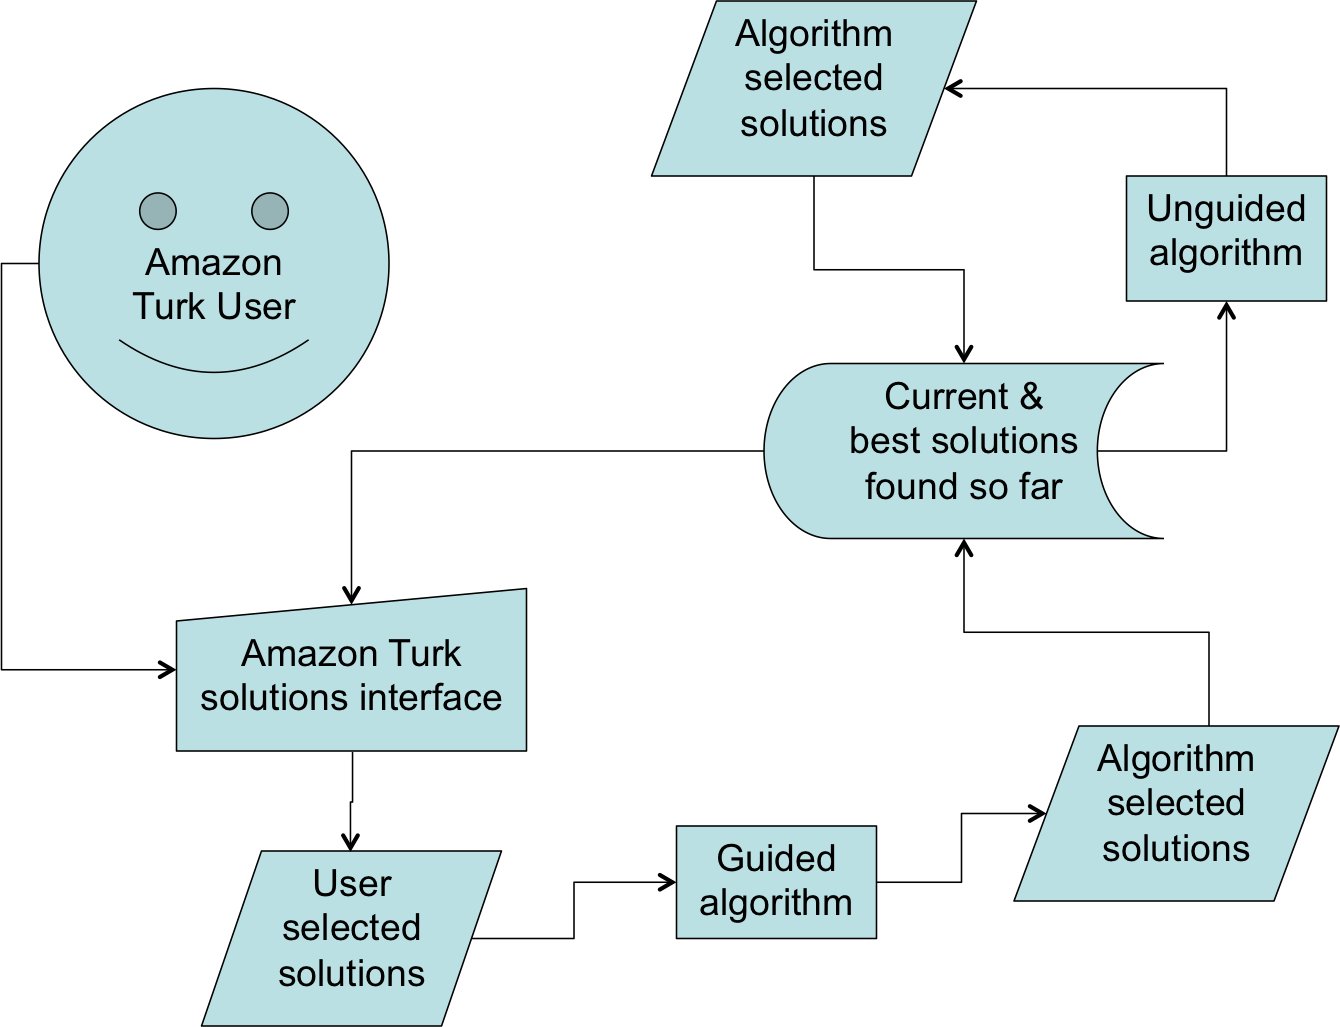
\includegraphics[width=4.5in]{HollowayDataFlow}
  \caption{CSIC data flow between user and algorithm.}
  \label{fig:data_flow}
\end{figure}

\subsection{User Interface}

In the user interface, the user is presented with a list of solutions from which he can make his selection.  The \index{solution symbolic representation}solutions are the strings of arbitrary symbols in Figure \ref{fig:CSIC_UI}.  Each solution is represented symbolically, so the user has no contextual clues as to what the problem is that he is attempting to solve.  This is done in order to create a \index{context independent interface}context independent interface that can be used for a wide variety of problems and algorithms. The only information to which the user has access is similarities between solutions (as shown by similarities in symbols) and the value of each solution. Once the user selects a set of solutions, he picks the type of variation operators to apply to the solutions, and then presses ``GO'' to have the algorithm, as shown in Algorithm \ref{alg:stochastic_global_solution_search}, create a new set of solutions.  Dembski's work implies that even with only this information it is possible for the user to be able to provide active information to the search algorithm because a prior external source of information is unnecessary to add active information to the search since the user is an intelligent agent.

The types of operators have different credit costs, since some operators discover more information about the problem than others. It is important to track the amount of information with which the user is making his decisions in order to fairly compare his performance to that of the unguided algorithm.  The \index{user reward}user is rewarded based on whether this new set of solutions improves over the best solutions found so far.  

\begin{figure}[!t]
  \centering
  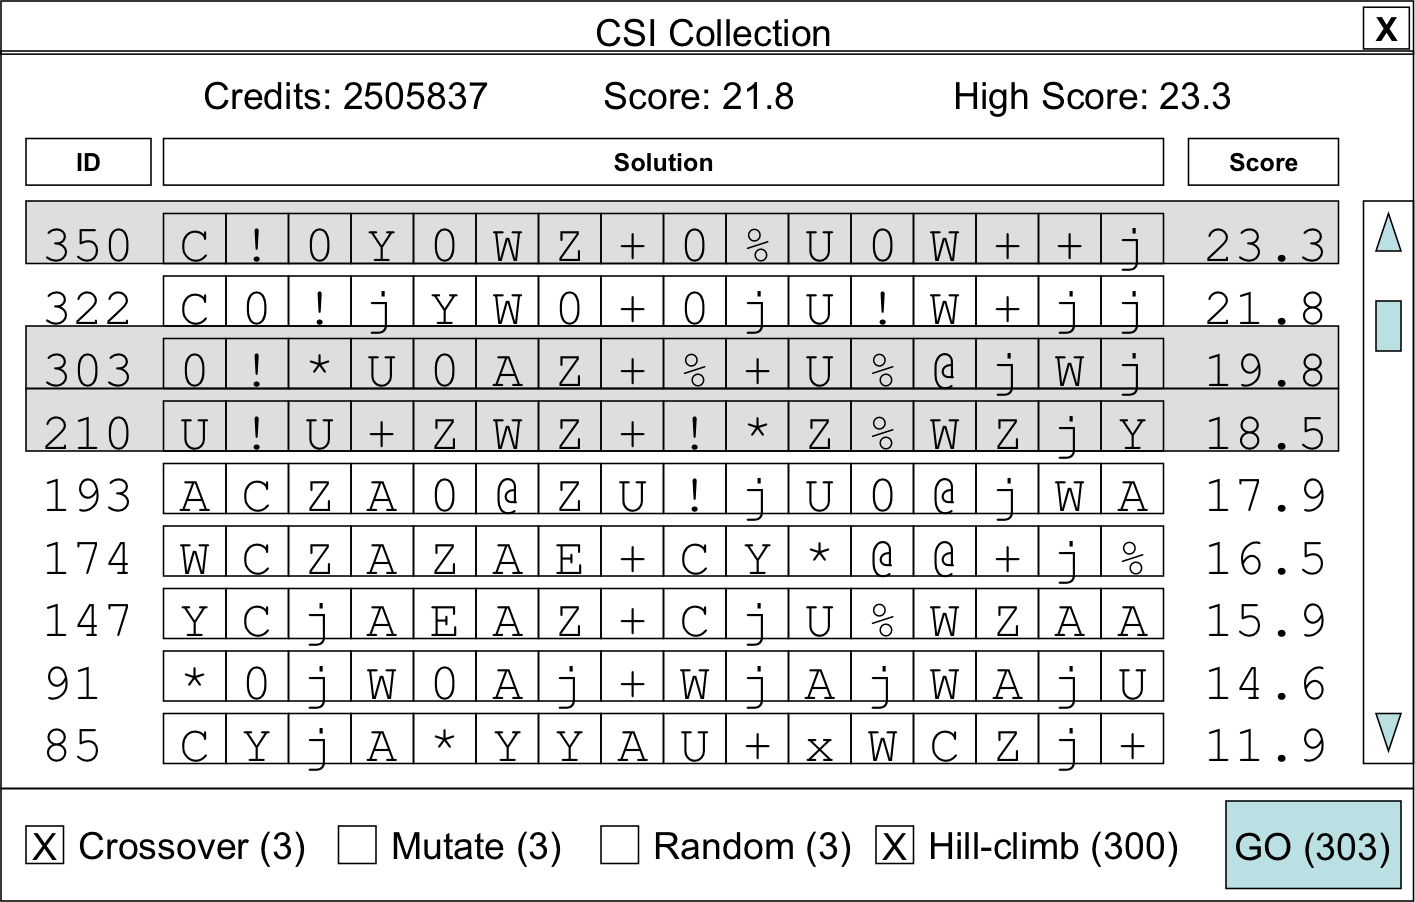
\includegraphics[width=4.5in]{HollowayCSICUI2}
  \caption{User inteface concept for CSIC.}
  \label{fig:CSIC_UI}
\end{figure}

The actual implementation in Figure \ref{fig:website_UI} is a simplified version of the interface shown in Figure \ref{fig:CSIC_UI}, since it is used by people on the Amazon Turk service.  Due to the low wage for using the interface, they cannot be expected to spend a long time trying to understand the intricacies of different variation operators.  Accordingly, credits are done away with since the same operators are used in every iteration.  Additionally, the numerical score is replaced with a visual indication of solution value, where higher valued solutions have a greater number of stars.

Otherwise, the basic idea is the same between the \index{actual and conceptual interfaces}actual and conceptual interfaces.  The users select solutions to guide the search algorithm, and then press ``GO.''  The users are paid a basic wage for using the webpage and are rewarded with a bonus based on the value of new solutions discovered.  The intent is to financially incentivize the users to discover highly valued and highly unique solutions. 

\begin{figure}[!t]
  \centering
  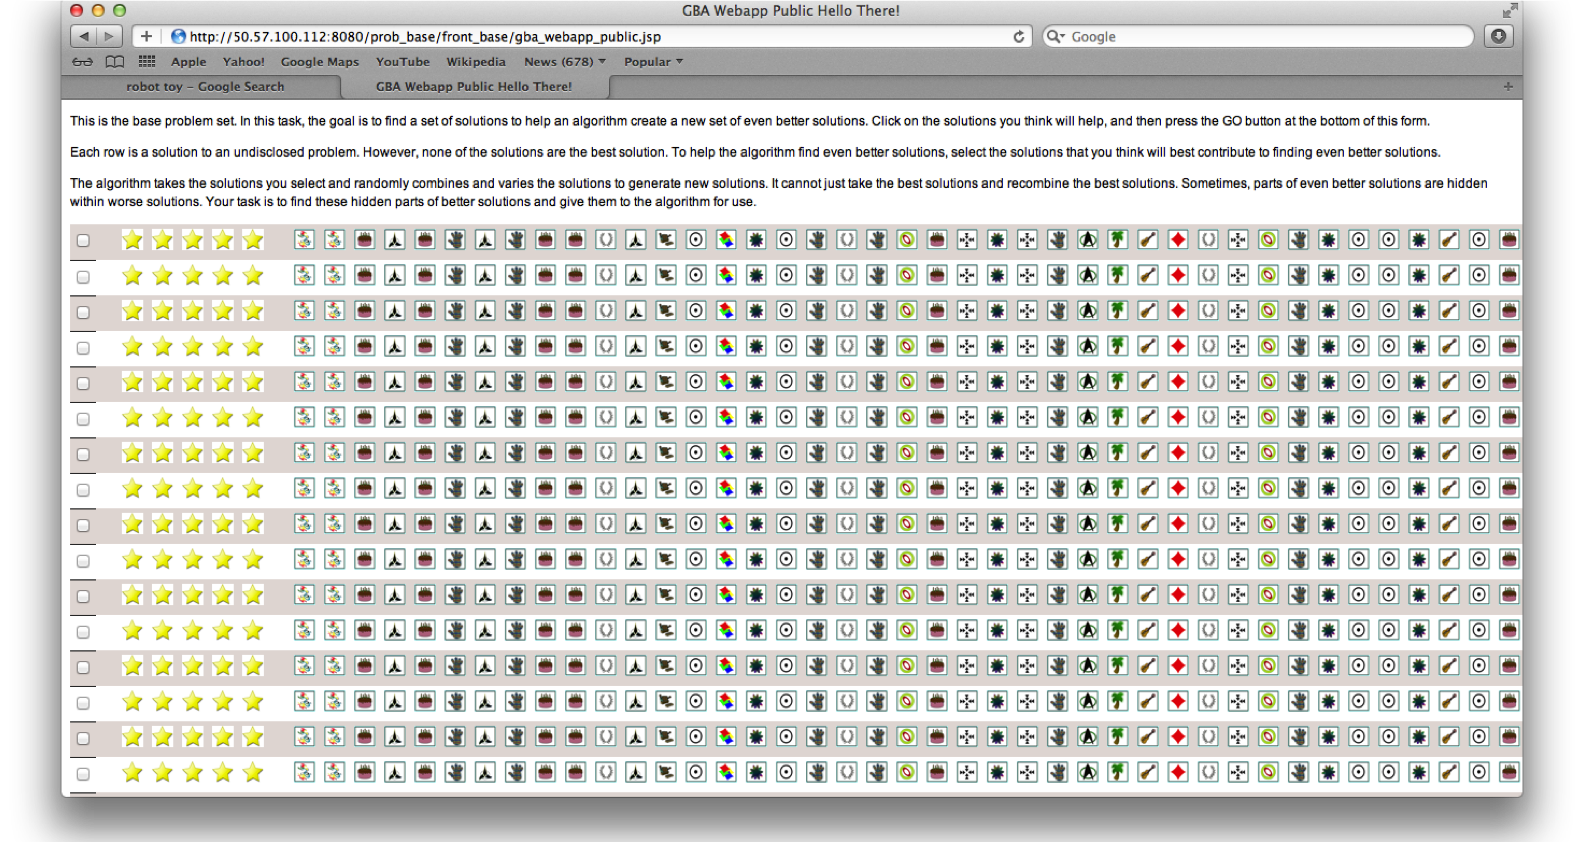
\includegraphics[width=4.5in]{HollowayWebsiteUI}
  \caption{Actual user inteface website.}
  \label{fig:website_UI}
\end{figure}

\subsection{Problem}\label{sec:problem}

CSIC is used to find the prime factors that generate keys for an asymmetric cryptosystem.  There is no known correlation between finding prime factors and multi-objective genetic algorithms, nor with human input during the selection phase.  This means the problem and algorithm together meet the criteria for the ANFLT to apply. 

Breaking asymmetric encryption is also an extremely hard problem, which is why it forms the basis of much information transmission security.  The asymmetric cryptosystem is RSA \citep{cormen01:_introd_to_algor}.  The genetic algorithm uses a multi-objective fitness function to measure how close a solution is to the correct set of primes.  To find the primes, the fitness function is given access to a true plaintext and true cyphertext. The two objectives are:

\begin{enumerate}
\item \emph{Matching encrypted bits}. The plaintext is encrypted using the keys generated by the solution primes.  This encrypted text is then compared with the true cyphertext, and the number of matching 1 bits are counted.  The 0 bits are not counted because they generally overwhelm the number of 1 bits.

\item \emph{Matching decrypted bits}. The true cyphertext is decrypted using the solution keys, and its accuracy is measured as for the previous objective.
\end{enumerate}

\section{Results and Conclusion}
The guided genetic algorithm received 500 human inputs from the Amazon Mechanical Turk service.  The human input contributed 1 out of 18 superior solutions found (Figure \ref{fig:results}).  The one solution found by a human was also found by the algorithm.  However, the logs show all human input consisted of selecting every single solution, which can be replicated by an algorithm.

\begin{figure}[!t]
  \centering
  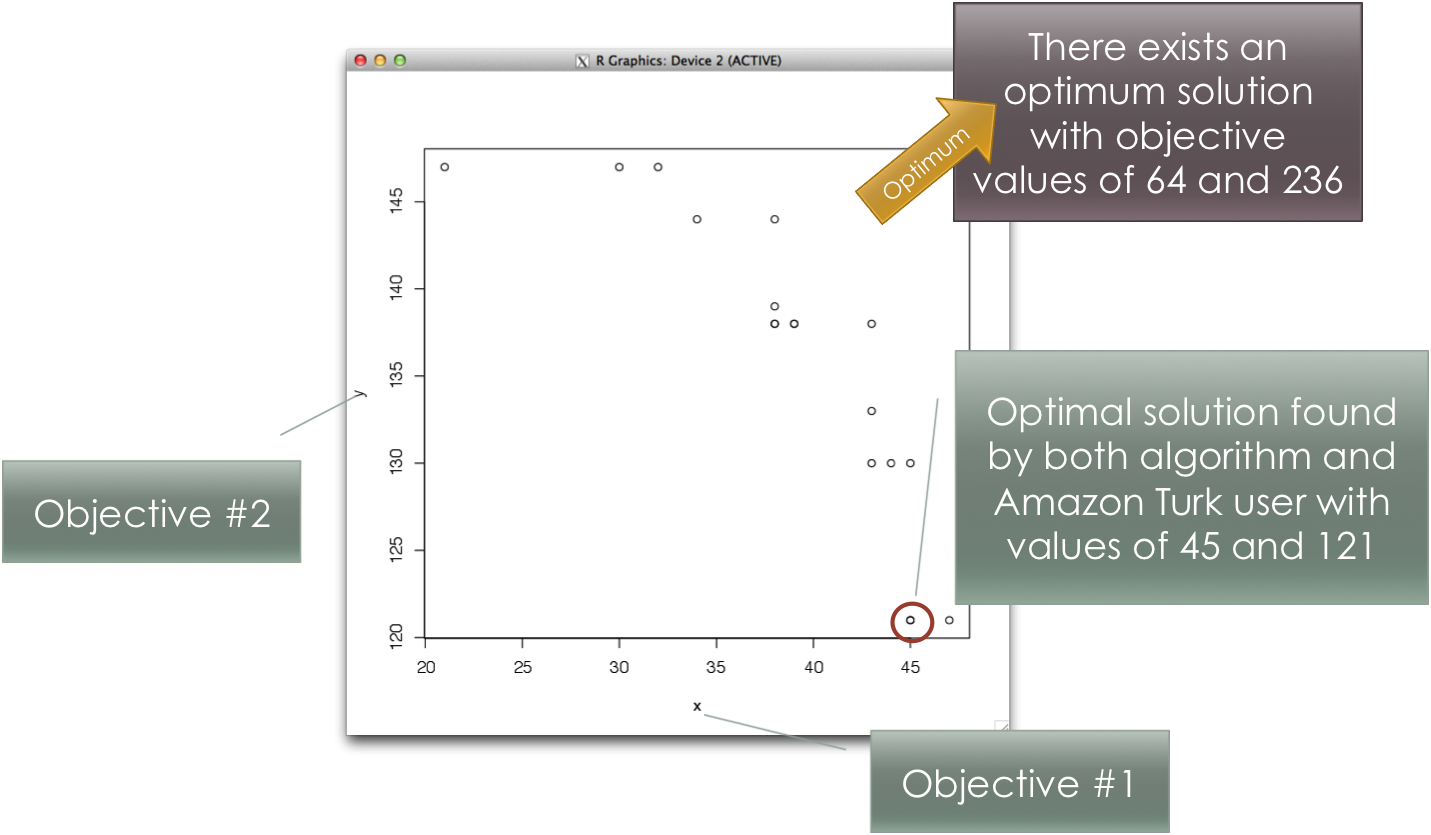
\includegraphics[width=4.5in]{HollowayResults}
  \caption{Best solutions found from Amazon Turk experiment.  The objectives are described in Section~\ref{sec:problem}.}
  \label{fig:results}
\end{figure}

This result did not validate the hypothesis, though the failure is  due to methodological factors, as will be discussed in Section \ref{sec:future-work}.  Since both the human and algorithm discovered the same solution it is not clear the solution was originally found by the human.  Thus, in terms of the FI metric in Section \ref{sec:solution-approach}, it is not possible to say whether the human outperformed the algorithm.

\section{Theoretical Objections}\label{sec:objections}

While the methodology for CSIC is still in its infancy, and its efficacy has yet to be demonstrated, there are also theoretical objections to the concept that have been or could be raised.  In the following section I attempt to answer these objections.  In all of these objections I assume CSI, or active information, cannot be created by algorithmic sources.  Additionally, I assume active information is a subcategory of CSI.

\subsection{Objection: Human intelligence is an algorithm with already high amounts of CSI}

One objection to this methodology is that human intelligence is an algorithm that \emph{already contains} high amounts of CSI, especially since the ANFLT does not rule out the possibility that a proximate algorithmic information source is available.  It might be the case that human minds are highly tuned algorithms for particular difficult problem domains.  Consequently, humans will outperform all current state of the art algorithms in these domains, but this does not preclude human intelligence being algorithmic.  This objection holds even in the case of the ANFLT.

Such an objection is valid.  The CSIC experiment cannot categorically rule out the possibility that human intelligence is a kind of algorithm.  However, CSIC can provide an \index{inference to the best explanation}inference to the best explanation between two competing hypotheses.  The first hypothesis asserts that the proximate cause, human intelligence, created the information.  The second hypothesis states that a more remote intelligent agent created the information.

To determine which hypothesis is better supported by a positive result in the CSIC experiment, I propose the \index{principle of minimal CSI creation}principle of minimal CSI creation.  The principle is analogous to Ockham's Razor.  This principle states in the case where the creation of CSI is presupposed, the explanation relying on the least amount of CSI creation is prefered.

The first hypothesis relies on less CSI creation, since the human only creates CSI for a particular problem instance.  Hypothesis two requires the creation of enormous amounts of CSI covering all possible problem instances the human might encounter.

 Consequently, while the CSIC experiment does not rule out algorithmic human intelligence, it does show that supra-computational human intelligence is the best explanation of a positive result. 

\subsection{Objection: Supra-computation does not imply effectiveness on all problems}
Another objection to this methodology is that even if human intelligence is supra-computational, this does not imply that it is necessarily effective on all possible problems.  It could be performing supra-computational actions which are still limited in scope, and thus preventing its use in arbitrary problems. This objection is also valid.  Consequently, the question is in which problems do humans demonstrate supra-computational abilities?  One way to answer this question is experimentally, by having humans work with different problems and seeing in which instances supra-computational abilities are exhibited.  This is the intent of the CSIC experiment.  There is no presumption supra-computational abilities will be demonstrated, only a presumption that it is possible to detect such abilities within the experiment. 

Research by \citet{bartlett11:_using_turin_oracl_in_cognit_model} suggests that even if humans do demonstrate supra-computation, such a capability may depend on existing information, such as axioms about the problem domain.  If true, then the almost complete removal of context in CSIC may render the user incapable of contributing active information to the search algorithm.

\subsection{Objection: Supra-computation is only exhibited in context dependent interactions}

This objection states that the removal of almost all context in CSIC is a methodological problem because experience seems to indicate that supra-computation only occurs within situational contexts.  A solution can only be created when the problem is contextually understood.

However, the observation is not always true.  One scenario similar to CSIC where information is created is learning to read.  When people learn to read a language, they are presented with a string of symbols without an inherent context.  They learn the meaning of the symbols through external responses, such as getting affirmation when mapping the symbols to the correct action or object.

\subsection{Objection: Supra-computation requires holistic \mbox{reasoning}}

This objection states that in order to solve a problem the person solving must not only know the problem, but also understand why the problem exists. Since the user of CSIC neither knows nor understands the problem at hand, he will be unable to solve the problem.

There is a degree of holism available in CSIC, as the user can see many solutions and valuations and thus look for overarching patterns. The user can understand at a very abstract level the characteristics of good and bad solutions.

\subsection{Objection: Fitness function in experiment cannot factor primes for RSA keys} 

This objection is quite likely correct.  However, even if correct, if human interaction improves the solutions beyond the algorithmic limits, then the experiment achieves a positive result.  On the other hand, better choices of problems, such as well understood pedagogical problems, would greatly improve the experimental design.  

RSA cracking was chosen for this experimental investigation mostly because the applicability of solving this problem is much easier to explain to a lay audience than more pedagogical problems.  Additionally, a successful result for this problem would have direct, groundbreaking relevance for software engineering.

\section{Future Work}\label{sec:future-work}

While the essential methodology and implementation of CSIC have now been created and tested, many areas of improvement remain.  Additionally CSIC must be compared to alternatives to see if CSIC is truly effective and beneficial.

The main improvement is verification whether the Amazon Turk input is truly human generated, and whether the users are actually trying to find patterns.  Users have been known to script Amazon Turk jobs, and without such verification in this case it is not possible to know with certainty whether the input is human generated.  When the logs from this experiment were analyzed, it turns out the Amazon Turk users were just selecting all the solutions and not trying to find patterns in the solutions.  To provide a cleaner environment for experimentation, the guided and unguided algorithms should be separated.  Additionally, the data logging needs to be time-stamped.

The algorithm and problem used in the experiment can be improved in numerous ways.  Pedagogical problems and algorithms should be used to compare the effectiveness of CSIC to the current state of the art.  Practical problems where search algorithms have already proven effective should be explored to see if CSIC can provide additional benefit.  CSIC should also be compared to contextualized human powered search algorithms, such as Foldit, to see how the addition of context affects search effectiveness.  

Different forms of motivation should be explored.  The Amazon Turk interface relies on a financial motivation, which motivates users to cut corners and perform the task in the fastest way possible.  Such motivation does not encourage users to find extremely good solutions.  If the interface is in the form of an entertaining game users are better encouraged to find good solutions.  Furthermore, a simplified explanation of the cutting edge relevance of their work provides an intrinsic motivation, and encourages innovation as demonstrated by significant user innovation in \index{Foldit}Foldit \citep{moore12:_foldit_game_leads_to_aids_resear_break}.

\eandmbibliography{HollowayLibrary}


\chapter[Roles of Engineering and Metaphysics]{The Independence and Proper Roles of Engineering and Metaphysics in Support of an Integrated Understanding of God's Creation}

%% FIXME - check dash sizes
%% FIXME - need to look at new references

\author{Alexander R. Sich, Ph.D.}

\begin{abstract}

The speculative (theoretical) sciences---including mathematics, natural sciences, and \sbf{metaphysics}---study the world independent of human volition, calling us to recognize the truths obtained as valuable in their own right. Indeed, these disciplines are ordered to ``understanding-thinking'' as an end in itself. The \sbf{engineering} disciplines, in contrast, are productive sciences ordered to ``understanding-making''---not as ends in themselves but to achieve practical ends \semph{per our wills}.

One distinguishes each particular natural science and engineering discipline by the subject matter each studies. Physics studies all forms of \sunder{natural} \semph{non-living} matter in physical motion by modeling ``objects'' according to mathematical formalisms while employing \semph{univocal} terms such as force, energy, mass, charge, etc. Biology studies all \sunder{natural} \semph{living things}. Engineering disciplines apply knowledge gained from the natural sciences to achieve practical ends---to the \semph{making} of \sunder{artificial} \semph{things} (artifacts). (Principles of motion of \sunder{natural} things are \semph{immanent to them}, whereas artifacts' principles of motion are imposed \semph{externally}.)

The knowledge obtained by the natural sciences and engineering disciplines is limited because they \semph{all} presuppose certain extra-scientific concepts and principles. These concepts and principles cannot be derived from any of the natural sciences themselves, for that would be circular. Moreover, the scientific method cannot validate its own ability to guide us to truths about creation: it cannot be the epistemic arbiter of all knowledge---otherwise known as the non-scientific pseudo-philosophy of scientism.

It falls to \sbf{metaphysics} to study the most general principles common to all \sunder{contingent beings}---whether natures or artifacts. For example, it is not the reduced understanding of motion studied by physics through physical efficient causality that metaphysics studies, but all manifestations of change \semph{qua} change. Metaphysics does not ask, ``\semph{how} do objects change?'' but ``\semph{what} is change?'' Metaphysics studies reality in ontological terms (hence, also employing \semph{analogous} terms), for it must understand what being, change, substance, accident, cause, potency, act, essence, etc. are in their widest throw. Moreover, metaphysics cannot be reduced to a crude synonym for ``world-view'': it is a rigorous speculative science that \semph{inter alia} animates the coordinating role a realist \sbf{philosophy of nature} plays for the particular natural sciences and engineering.

It falls to a \sbf{realist philosophy of nature} to study the most common principles of the \sunder{natural sciences}: to provide the foundational principles which \semph{all} particular sciences and engineering disciples presuppose, there must be a way of knowing nature whose subject matter concerns the \semph{principles and causes of natural} things insofar as they are natural---that is, subject to \semph{change} per principles immanent to themselves. A realist philosophy of nature therefore has the same \semph{general} subject matter as the natural sciences, but it applies \semph{general philosophical} (rather than \semph{specific scientific}) methods to study nature, and it does not suffer the operational restrictions of \semph{methodological naturalism}.

\sbf{Philosophy of nature} must be distinguished from \sbf{philosophy of science}---the latter which studies \semph{systems of reasoning about natural things}. It must not be confused with \semph{philosophical naturalism}, nor should it be conflated with the term ``natural philosophy'' as used during the Enlightenment, whose antecedents reflect a slow, incremental drift from a unified understanding of nature into the fragmentary and highly-specified particular sciences we observe today.

\end{abstract}

\section{Introduction}

\introquote{\textit{You arranged all things in measure and number and weight.}} 

\introquoteref{Wisdon of Solomon 11:20}

Metaphysics and engineering must be carefully distinguished to understand their subject matters and proper roles in support of an integrated understanding of God's Creation, and to avoid confusion that stifles such understanding, which in turn leads to an erroneous view of reality.

Today, predominate schools of philosophy are, at best, indifferent to, but more likely positively skeptical---if not openly hostile to---metaphysical thought. Metaphysics is unfortunately not understood as the classical systematic study of being as being and the properties that apply to all beings, but a grab-bag of diverse problems (e.g., free will, the existence of God, mind-body, ``eviscerated'' causality, etc.), whose only common bond is that they cannot be solved by the natural sciences, phenomenology, or other hyper-specialized disciplines.

Perhaps more unfortunately, metaphysics is often reduced to a crude synonym for ``worldview'' or ``philosophy''---a cheap, pseudo-mystical account relegated to dime-bookstores. Consider, for example, the description provided by this conference's website, which are followed by brief comments that will be expanded upon in this paper:

\begin{quote}
In short, metaphysics \semph{is} about the ultimate nature of reality. It includes many aspects of reality that are generally skipped over in standard physics, such as choice, creativity, morality, aesthetics, etc. While many engineers implicitly use their understanding of metaphysics when developing solutions, our goal is to move that thinking into explicit terms, so that those parts of our understanding can be better explored and systematized. Science is often bound by a methodological disregard for anything other than efficient causes. However, as engineers, our job is to include the whole of reality, and provide solutions that incorporate our entire knowledge of reality. Therefore, this conference aims at starting the discussion of how the fields of metaphysics and engineering influence each other.\cite{aboutconference}
\end{quote}

\begin{enumerate}
\item Indeed, metaphysics is about the ultimate nature of reality, but only in a qualified sense: it studies the principles of all contingent existens (beings) and supports theological reflection upon revealed knowledge.
\item There is no place for the study of choice (free will) in physics because physics studies an altogether different subject matter.
\item The natural sciences are \semph{not} bound by a methodological disregard for all but efficient causes. The natural sciences also incorporate physically-based material causes and a rarified version of the formal cause as manifested through mathematics.
\item It is most manifestly not the objective or responsibility of engineering to include the whole of reality: engineers \semph{make artifacts} based upon refined and highly focused natural scientific knowledge. \semph{Scientism} is the pseudo-philosophical notion that the modern empirical sciences (MESs) are the epistemic arbiters of all knowledge, so we want to avoid imputing a similar role to engineering\ldots which will result in \semph{engineergism}.
\end{enumerate}

\section{What Are the Sciences and How Are They Distinguished?\footnote{This section summarizes salient principles presented in sections II-IV of Mortimer J. Adler, \textit{Aristotle for Everybody}, (New York: Macmillan, 1978), 23-167.}}

What this begs are some important questions that will permit us to avoid the sentimental and erroneous notion of a particular discipline's attempts to pull the knowledge of all things into itself:

\begin{itemize}
\item What is ``science''?
\item What is ``engineering''?
\item What is ``metaphysics''?
\end{itemize}

A correct response to these questions---which, at the end of the day, should provide clear definitions---is part of the broader question that serves to demarcate the bounds of these disciplines responding to its own question: to what extent do each of these disciplines span the realm of human knowledge?

Man is a reasoning being because the definition (i.e., the logical genus and specific difference) of a \semph{human being} is a \semph{rational animal}. The very first sentence of Aristotle's \btitle{Metaphysics} strongly echoes what man is by his very nature: ``All men by nature desire to know.''\footnote{``\emph{All men by nature desire to know}. An indication of this is the delight we take in our senses; for even apart from their usefulness they are loved for themselves; and above all others the sense of sight. For not only with a view to action, but even when we are not going to do anything, we prefer sight to almost everything else. The reason is that this, most of all the senses, makes us know and brings to light many differences between things.'' (I.980a21)} Moreover, we as humans are commanded by Christ not to leave our brains at the door of knowing and loving God: ``And thou shalt love the Lord thy God with all thy heart, and with all thy soul, and \semph{with all thy \sbf{mind}}, and with all thy strength: this \semph{is} the first commandment.'' (Mark 12:30 echoed in Luke 10:27) However, the \semph{kind} of thinking man undertakes differs importantly depending on the \fword{telos}---the end sought. As such, there is a crucial logical distinction based on the role of truth in all human activities, i.e., the distinction of seeing man as a

\begin{itemize}
\item knower for the sake of knowing
\item doer or ``acting individual''
\item maker or ``builder''
\end{itemize}

Stated another way, the \semph{kind} of thinking man does (1) as a knower for the sake of knowing (i.e., productive of knowledge) differs from (2) the thinking done to act morally, socially, or politically (i.e., productive of actions), differs from (3) the thinking done to make things (i.e., productive of artifacts). In the sphere of \semph{knowing}, we are concerned with \semph{truth as truth}; in the sphere of \semph{doing} we are concerned with \semph{truth as action} (characterized as good and evil, right and wrong, etc.); in the sphere of \semph{making}, we are concerned with \semph{truth as beauty} (producing things that are ``well made'').

Indeed, the \semph{true}, the \semph{good}, and the \semph{beautiful} are among those few but extremely important metaphysical terms called ``transcendentals''---terms which apply to all contingent beings to the extent they exist, and as such are not \semph{valuative} but ontological.\footnote{Transcendentals are properties of \textit{all} contingent beings to the extent they exist. In typical accounts, there is the existent (\textit{ens}) itself, and then being is then said to be one, good, and true (\textit{unum}, \textit{bonum}, \textit{verum}), although St. Thomas Aquinas includes two more: thing and something (\textit{res}, \textit{aliquid}) in \textit{Disputed Questions on Truth}, q.1 a 1 (http://dhspriory.org/thomas/QDdeVer1.htm).  The transcendentals are ontologically one, thus they are convertable: where there is truth, there is also beauty and goodness.} A fly is ``beautiful,'' but not as beautiful as human---not in an emotional, aesthetic, or ``valuative'' sense but in the sense of an ontological hierarchy: a human exists ``more''---has a greater claim to existence---than a fly. A rock, in turn and in this sense, is ``less'' beautiful than a fly, but again not an emotional, aesthetic, or ``valuative'' sense. God, does not ``exist''---He IS Existence Itself, without a hint of potency, utterly simple\ldots and in that sense He is Beauty Itself.\footnote{The ultimate aim of metaphysics is knowledge of God as the human mind can acquire. Aquinas uses analogous names to give an account of the divine attributes such as wisdom, justice, mercy, being, one, true, good, etc. See Summa Theologiae I.13.}

So how are the relevant portions of reality demarcated for study among the various scientific disciplines? Really, what distinguishes (or should distinguish) the particular sciences is---employing logical terms of art---the \semph{subject matter} (sometimes called ``proper object'') studied by each.\footnote{St. Thomas Aquinas, Commentary on the Posterior Analytics [of Aristotle], Lectio 21, Caput 12 (77a36-77b15) ``The Questions, Responses And Disputations Peculiar To Each Science,'' see http://www.josephkenny.joyeurs.com/CDtexts/PostAnalytica.htm\#21} In other words, the distinction is not principally rooted in what we may devise as an \fword{a priori} classification scheme, but in the very objects studied. In other words, the question ``what \semph{kind} of an object is that?'' should lead the distinction. For example, is a ``neutrino'' the same \semph{kind} of thing as a ``frog,'' or a ``Venus flytrap'' the same \semph{kind} of thing as a ``triangle,'' or is DNA the same \semph{kind} of thing as ``design''? What this implies, of course, is that the particular sciences by themselves cannot form a basis for those distinctions, for that would be circular reasoning.

(Brief digression: at this point the reader should sense just how different the particular sciences and metaphysics are from engineering: to repeat, the former seek knowing for its own sake; the latter seeks knowing in order to make.)

To help bring out the important distinctions (and hence provide a basis for classification), the sciences will be differentiated based on the subject matter and on the outcome or result. The first question must be, ``what is science?'' Classically and in its widest throw, science is ``certain knowledge through causes'' or ``mediate intellectual knowledge obtained through demonstration.'' What this means is that theology and philosophy are also sciences, although they employ different methodologies, instrumentation, and means by which to achieve their end---truth about the real world. Just as one does not employ a telescope to study bacteria, one does not employ physics to study free will or the Transfiguration.

Now we may ask, ``what does science do?'' The answer to this question was introduced above, but we may now attach names to the ``doing'': (1) the ``theoretical'' or ``speculative'' sciences are those that study truth as truth; (2) the ``applied'' sciences study (a) truth in doing/action, and (b) truth in making/beauty; and (3) the methodological sciences study how we guide our reasoning to truth in both (1) and (2).

Finally, we distinguish what exactly the particular sciences study. This is perhaps best depicted in the diagram below which relates the two major distinctions noted above. In addition, the diagram will help us to distinguish the speculative (theoretical) sciences through their subject matter by means of the level of abstraction.

\begin{center}
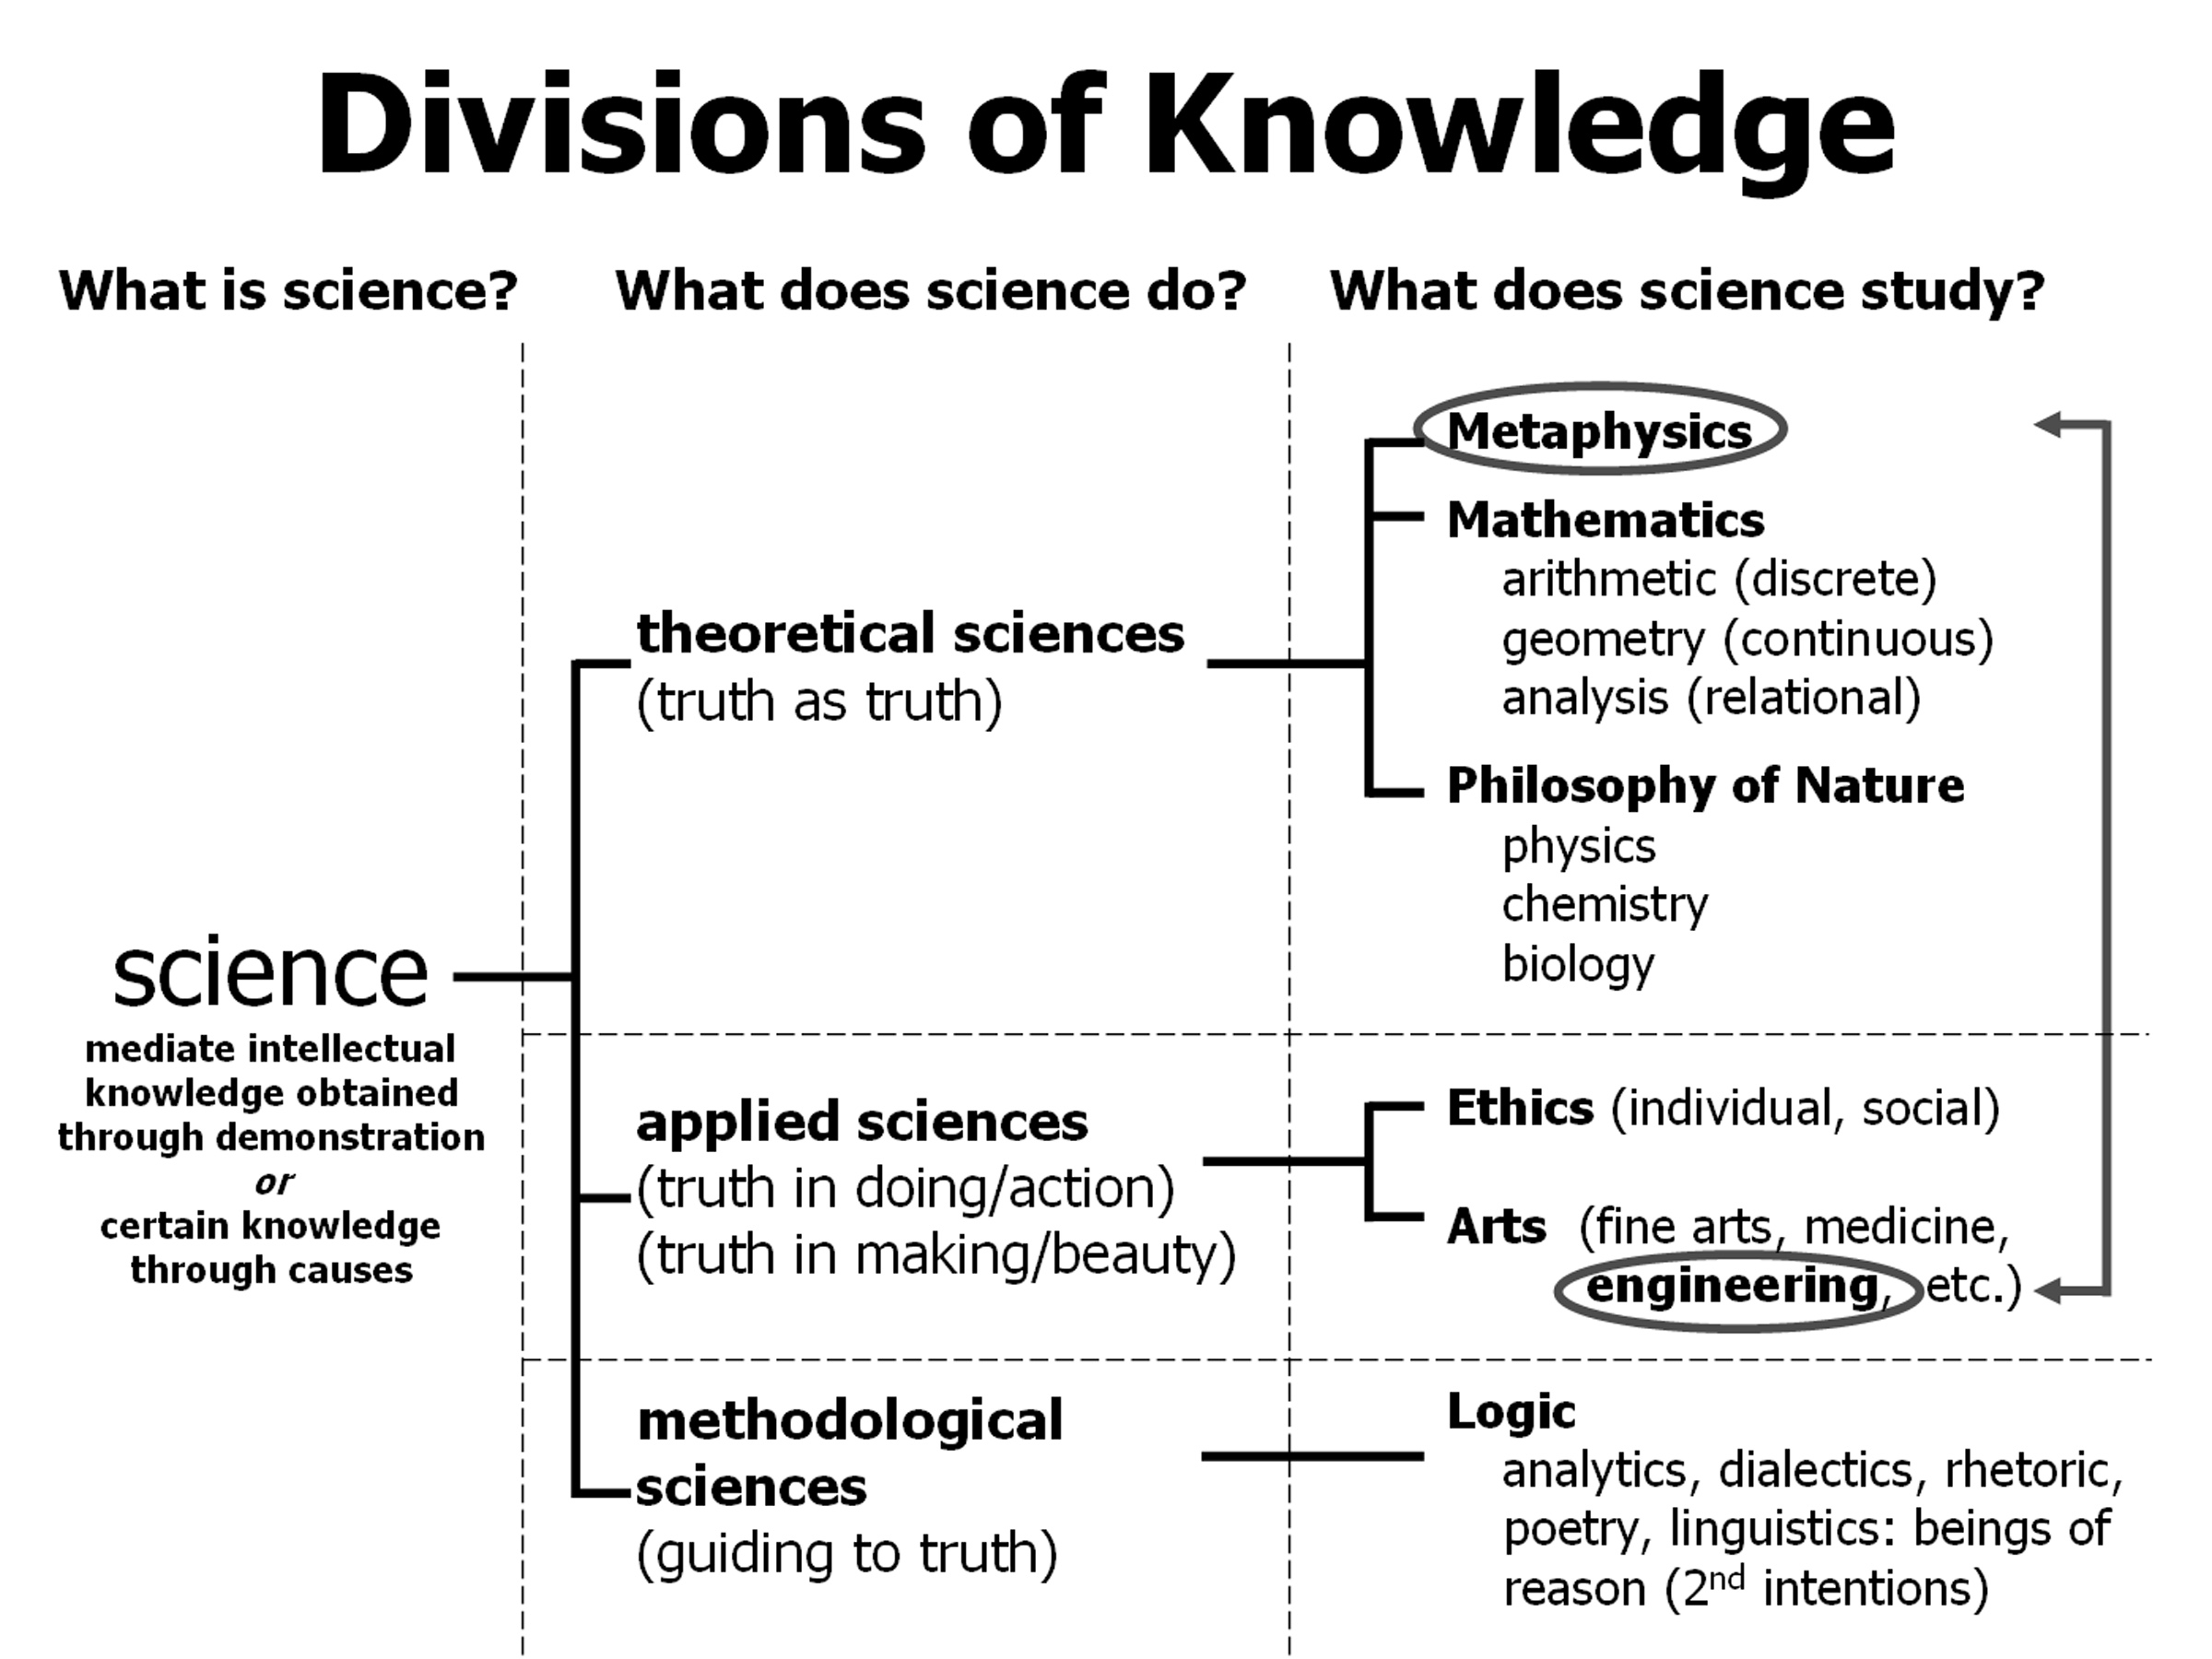
\includegraphics[scale=0.6]{sich_science_taxonomy.jpg}
\end{center}

All the particular (in the sense of ``individual'') sciences study different aspects of being. The question then becomes ``what are those \semph{fundamentally} distinguishing aspects or characteristics?''

Consider the speculative sciences. A discipline under the speculative sciences is the \sunder{philosophy of nature}, under which in turn can be distinguished the natural sciences:

\begin{itemize}
\item \sundertitle{Physics} studies matter in motion by modeling physical ``objects'' according to mathematically-formulated deterministic mechanisms;\footnote{Note for quantum mechanics one must be careful to distinguish the mathematical formalism employed to describe the behavior of objects that are highly affected by observation (measurement) from the natures of those objects. Epistemic limitations (in measurement) currently force us to employ statistical mathematical formalisms to describe observed quantum phenomena, but this in no way dictates the ontological status of those phenomena. The wave equation of an electron, for example, is derived from the observation of a huge population of electrons under specific conditions, but it does not follow that an electron is---by its nature---a wave: some wave-like behavior does not imply wave-like nature. An example might clarify this: the mathematical formalism known as a normal function describing the shape of the collection of balls that have fallen through a Galton board in no way implies the balls themselves---by their nature---are ``spread out'' in space or whose motions are \semph{random} (i.e., without cause). The Copenhagen Interpretation commits a gross error in logic and scientific procedure by concluding that what cannot be measured exactly does not occur exactly: an epistemic principle was converted into an ontological principle.}
\item \sundertitle{Chemistry} is concerned with the composition, structure, and properties of matter, as well as the changes matter undergoes during chemical reactions;
\item \sundertitle{Biology} studies living things---examining their structures, functions, growth, origin, distribution, and classification.
\end{itemize}

\sundertitle{Mathematics}, as a science, stands apart from the natural sciences because it studies being from which all properties (philosophically: accidents) abstracted except quantity---either discrete or continuous. In other words, mathematics studies being as quantified. \sunder{Metaphysics}, a science as well, stands above all---not just abstracting but \semph{separating} everything from being except those aspects shared by \semph{all} beings. \sundertitle{Theology} is a science: its subject matter is knowledge of God and Divine things obtained through philosophical reflection and argumentation. \sundertitle{Logic} studies beings of reason or second intentions. It is the science that seeks knowledge for its own sake and is productive of something for it organizes and guides reasoning to the truth. It is from this that we better see how levels of abstraction (from real beings to the object studied) distinguishes the sciences---yielding the subject matter of each of these disciplines.


\section[The Role of Abstraction]{The Role of Abstraction in Distinguishing the Particular Sciences\footnote{Many commentaries are available on the works of Aristotle and St. Thomas Aquinas that summarize the degrees of abstraction that distinguish the speculative sciences. See, for example, Jacques Maritain, \btitle{The Degrees of Knowledge}, trans. Gerald B. Phelan (New York: Charles Scribner's Sons, 1959): 35-36 and Rudi A. Te Velde, \btitle{Aquinas on God: The ``Divine Science'' of the \textrm{Summa Theologiae}}, (London: Ashgate Publishing, Ltd., 2006): 51-53.}}

(1) At the first level of abstraction, ``particular'' matter is left behind to focus upon ``general'' matter---where ``matter'' is understood in the logical sense. For example, the focus is not upon this red apple but upon the general notion of redness (physics) or the general notion of apples (biology) \semph{universally} applied to all particular objects studied. For the philosophy of nature, any particular red apple is termed a \semph{primary substance} while the universal ``apple'' is a \semph{secondary substance}; redness is an \semph{accident} (the Aristotelian category ``quality'') that can inhere in many different real objects. Another example is Socrates (primary substance) vs. human being (secondary substance). This first level of abstraction---generally applied to the philosophy of nature---resolves being in the sensible and the subject matter is \fword{ens mobile} (changeable being), while the individual natural sciences discriminate even further as noted above but worth repeating:

\begin{itemize}
\item Physics studies \semph{natural} material ``objects'' undergoing physical changes
\item Chemistry studies \semph{natural} material objects subject to electron-based interactions
\item Biology studies \semph{natural} living things
\end{itemize}

``Natural''---or ``natures''---as the term is used here is not to be understood in the popular or ecological sense but as applied to those things in whom the principles for motion/change are immanent. \semph{Artifacts}, on the other hand, ultimately have their principles located externally to them. Stated philosophically, an acorn has the immanent capacity to actualize its nature into a mature oak tree.\footnote{For the distinction between natural things and artifacts: Aristotle, \btitle{Physics}, Book II, 192 b 9-18, 28. See also Eleonore Stump, ``Substance and Artifact in Aquinas's Metaphysics,'' in Thomas Crisp, Matthew Davidson, David Lander Laan, eds., \btitle{Knowledge and Reality: Essays in Honor of Alvin Plantinga}, (Springer Netherlands, 2006): 63-79.} A robot, which is technically termed an ``accidental unity,'' ultimately has its motion or change ``located'' (in the sense of ``explained'') as external to it: even a ``self-powered'' robot is not strictly that, for some external rational agent had to design the robot and impart upon it the ability to be ``self-powered.''

Notice also the use of the word ``object'' particularly as applied to physics. When physics studies motion,\footnote{To be quite precise, physics does not study motion in the same sense that biology does not study life: neither “motion” nor “life” are, respectively, the objects of these sciences. \textit{Physics} studies material \textit{\textbf{things} in motion}; \textit{biology} studies \textit{living \textbf{things}} (or \textit{\textbf{things}} that were once living). “Things” here are understood as real, extra-mental existents accessible to (observable by) the five external senses or the senses enhanced through instrumentation. Neither “life” nor “motion” are per se observable by the senses: we know “motion” and “life” exist, but only because we reflect upon the knowledge gained through the natural sciences, and that reflection properly belongs to the philosophy of nature. See, in particular, section IV paragraph 3 ahead.} it simplifies the things studied (termed an ``object'') in order to understand the motion, and then attempts to return to the fullness of reality by successively increasing the complexity of external influences. For example, a typical introductory Freshman-level physics course may pose the following problem: an \semph{object}, for which the final position is to be determined, is hurled into the air at such-and-such a speed in such-and-such a direction. It doesn't matter to physics whether that object is a marble, a howitzer round, or an elephant: physics does not focus on the essence (``whatness'') or nature of the object, and it doesn't need to\ldots nor can it. Once that basic level of motion is understood, one can then incorporate into the question other factors that will influence the motion: initial angular momentum, air resistance, expansion due to rapid heating, curvature of the earth, air currents, manufacturing flaws, etc., etc. In fact, given time, patience, and resources, one can proceed to any level of precision. \semph{But}, the full ontological import and essence of the ``object'' will never be captured by physics alone---let alone my mathematics.

(2) The second level of abstraction ``belongs'' to mathematics: all sensible aspects are left behind except the quantitative, and hence the beings studied are resolved not in the senses but in the imagination. Note that even highly abstract mathematical concepts (Lie groups, Fourier analysis, complex functions, etc.) must ultimately be reducible to discrete and continuous quantities abstracted from real objects. Mathematics is therefore the study of things that can be imagined and conceived without matter, not just the abstraction from the particular for the philosophy of nature and the individual natural sciences. The focus of mathematics is upon the first Aristotelian category of real being---quantity, again whether continuous (surfaces, volumes, etc.) or discrete (integers, countables, etc.) or relational (equations, inequalities, etc.).

Quantity, as the first accident of real being, is the basis for quality---the second accident of real being. For example, the average temperature of air in a room presupposes a non-point-like \fword{res extensa}---a thing spatially extended---and the ability to measure (quantify). Further, quality admits of degree; quantity does not. For example, no number (quantity) of kindergarteners adds up to the intelligence (quality) of Einstein.\footnote{It also makes for good jokes among scientists, e.g., 2 is equal to three for large values of two.} Finally, geometry, for example, is not concerned with the question whether a triangle (as imagined from some extra-mental object) is made of copper or of wood, but only with its absolute quantifiable nature, according to which it has three sides and three angles that add to 180 degrees in Euclidean (flat) space.

(3) The final level of abstraction is actually ``separation'': all material aspects are left behind or ``separated'' from that which can exist without matter. Angels, for example, are purely immaterial beings and as such cannot in any way be imagined, for imagination requires an image---a picture---in the mind. Metaphysical terms such as unity, substance, soul, potency, causes, etc. exist without matter as well because such concepts apply to all extra-mental existents. Metaphysics, therefore, does not study being as changeable (philosophy of nature) or as quantifiable (mathematics) but being as being, and hence such being can only be resolved through concepts in the mind. As such, metaphysics is the study of the foundational principles of all beings---those aspects shared by \semph{all} contingent beings.

In a strong sense, metaphysics is really at the heart of philosophy since it deals with the nature of reality in its widest throw. Metaphysics comprises two main areas or sub-disciplines: ontology and transcendental metaphysics. Ontology concerns itself with responding to the question ``what exists?'' while Transcendental Metaphysics concerns itself with the questions ``what is it for something to exist?'', ``are their different modes of existence?'', and ``if there are different modes of existence, what are the truth makers for these modes?'' More specifically, ontology attempts to formulate a complete list of all the fundamental categories of being, while transcendental metaphysics concerns itself with a fundamental understanding of essence, existence, nature, cause, etc., and the relationships between them, with the truth makers for modal claims, and with the transcendental attributes of being---attributes which apply to all beings simply as beings.

Consider the example of shoes. One can think of what is common to shoes, but one cannot draw it, i.e., quite literally one cannot imagine that commonality or universality known as ``shoeness'' shared among all shoes. As such, there is absolutely nothing which can be sensed---and hence measured---about ``shoeness.'' When one has an idea (not image!) of what is common to all shoes, of every shape, size, color, style, etc., one has grasped \sunder{conceptually} the form (formal cause---the ``whatness'')---the shoeness.

\section{Metaphysics: the Foundational Science}

So, metaphysics is the foundational philosophical discipline---quite literally \semph{the} foundational science. Whereas the modern empirical sciences (MESs) are the most fundamental form of knowledge we have because their objects are accessible to us through our senses, the MESs are neither the only form of knowledge nor the most important. All the particular (individual) sciences---including the productive sciences such as medicine and engineering and architecture---depend upon metaphysics for their ultimate presuppositions and basic principles. The particular sciences seek to understand their particular subject matters through the proximate ``ultimate'' causes within their particular domain. And, no science can prove its own proximately-considered first principles. There must be one foundational science (metaphysics) which seeks to understand all reality---all contingent beings---in terms of the universal properties of being as such.

Consider the example of \semph{change}, and the species of change called ``local motion'' (translational, vibrational/oscillatory, and rotational/circular) through the following example. If one were to query a group of one hundred people chosen at random how many of them were seismologist that have modeled tectonic subduction zones, the expected response would be one, perhaps two of those people. If one then asked the same group how many had experienced an earthquake, the response might increase to about fifteen people. If one were then to ask the group how many know \semph{what} motion is, or at least experienced it, the hands of all the people in the group would be raised. This example highlights the difference between the narrowly- yet deeply-focused work of scientists, those who have had special experiences and hence knowledge, and the common knowledge shared by all healthy individuals.

Motion (change of position of a material object as a function of time) for a physicist is relatively easy compared to the general notion of what motion is, for physics only asks ``how do things change/move?'' whereas the philosopher must ask ``\textit{\textbf{what} is} change in its widest throw?'' Motion for the philosopher is merely a species of change, for it is not merely a metaphor to assert, ``I was \semph{moved} by the beauty of my wife.'' There was a ``before'' when I was not moved, and then there was an ``after'' when my potential to be moved was actualized into reality---the reality of actually being in love. Hence, the most general definition (i.e., not the narrow physics-based definition) of motion is ``the reduction from potency to act, inasmuch as the object is in potency.''\footnote{According to Aristotle, motion must be defined as ``the act [entelechy] of that which exists in potency insofar as it is such'' (\fword{actus existentis in potentia secundum quod huiusmodi}), \btitle{Physics} 3.2, 201a27--29.} It was this general definition---based upon common experience accessible to all---that provide the foundation for physicists to do their good, mathematically-described work. Change had to be understood in its widest, most general throw before physics could narrow that understanding of change to study material objects in physical motion.

So, to revisit the three speculative sciences we can say

\begin{itemize}
\item \sundertitle{Physics} studies those things (material objects and physical phenomena) that have separate substantial (real, i.e., extra-mental) existence but are subject to change;
\item \sundertitle{Mathematics} studies those things free from change but which do not have separate substantial (real, i.e., extra-mental) existence: they exist only as distinguishable aspects of concrete realities. E.g., a tire's shape is a circle, the statistical distribution of students tests scores is described by a normal curve, etc.
\item \sundertitle{Metaphysics} studies those things that have separate substantial existence but are free from change---primarily the study of substances (as they are the primary mode of being): what aspects do all substances share?
\end{itemize}

\section{Quo Vadis, Engineering?}

Let us now focus our attention upon engineering as the applied science it is.

The metaphysician asks ``what is motion?'' The physicists asks, ``how do levers move under the influence of external forces?'' The engineer asks, how do I construct a structurally-sound bridge that will not move (within set parameters) under the influence of external forces?'' The differences between the questions asked, and hence the objects studied by these disciplines is profoundly different.

The goal of the speculative (theoretical or ``pure'') sciences is to conform one's mind to reality. The goal of the applied sciences is to conform one's actions to reality, and by them we know (a) which actions conform to reality, (b) what we ought to do, and (c) how and why we should act.

In fact, one can only be successful in the applied sciences to the extent one is successful in the pure sciences. Ethics or moral philosophy answers the questions what should we do and why? The arts (including engineering as productive of ARTifacts) are---nay, must be---subordinate to ethics: one must first decide what one ought to do (which implies knowing why); then and only then may one enter into the details of how to do it. For example, knowing how to abort a child cannot trump knowing whether to do so. Another example is out ability, through science and technology, to detect weapons of mass destruction in Iran through remotes sensing. But no natural scientific, technological, or engineering discipline can then determine whether and what should be done about those weapons.

The applied sciences are subordinate to the speculative sciences as the speculative sciences are subordinate to the science that provides their principles---metaphysics. The knowledge obtained by the natural sciences must precede the application of the knowledge through engineering, and in that sense engineering is subordinate to the natural sciences as well.

So let's add engineering to our taxonomy in terms of the relationship it enjoys with the speculative sciences.

\begin{itemize}
\item \sundertitle{Metaphysics} is the study of being as being.
\item The \sundertitle{modern empirical sciences} study the metrical properties (quantified observables) of changeable, material objects---objects particular to each natural science.
\item The \sundertitle{philosophy of nature} stands between these two disciplines as the study of all changeable beings---of the general properties of all real (extra-mental, substantial and accidental) existents.
\item The \sundertitle{engineering disciplines} apply the knowledge gained from the natural sciences to achieve practical ends---to the making of artificial things (artifacts---\semph{not} natures).
\item The \sundertitle{philosophy of science} studies systems of reasoning (methodological epistemology) of natural things.
\end{itemize}

So, we see metaphysics is ultimately connected to engineering because it studies the first causes and principles of all beings---including those things studied by the modern empirical sciences and engineering.

However, the modern empirical sciences are ``closer'' to metaphysics because

\begin{enumerate}
\item they are speculative (theoretical) in the same way metaphysics is
\item the modern empirical sciences provide real-world knowledge for metaphysics to reflection upon
metaphysics, through natural philosophy, provides the modern empirical sciences with foundational (proximate ``first'') principles
\end{enumerate}

In contrast, engineering is ``located'' further from metaphysics because

\begin{enumerate}
\item it is applied knowledge (productive of artifacts) rather than speculative
\item it depends upon the MESs to provide knowledge of the real world
\item it provides metaphysics no direct substantive knowledge of the real world upon which to reflect
\item metaphysics---through the philosophy of nature and the modern empirical sciences---provides engineering with foundational principles
\item it is subject to the constraints of the practical sciences (e.g., ethics)
\end{enumerate}

Productive reasoning involves having what one might be tempted to call ``creative'' ideas. In fact, productive ideas are based upon some understanding of the forms that matter can take, supplemented by imaginative thinking about such details as sizes, shapes, and configurations. Scientific knowledge can indeed be applied productively: scientific knowledge, through \semph{technology} (= scientific know-how), provides us with the skills and power to produce things.

But the philosophical reflection that improves our common-sense grasp of the physical world in which we live gives us neither the skill nor the power to produce anything. Philosophy bakes no cakes and builds no bridges. So, is it ``useless'' in the Marxist sense? No. Echoing more strongly a previous point, philosophical knowledge lays the foundations of our thinking and can be ``used'' to direct lives and manage societies: philosophy animates for the sake of doing---not directly for the sake of making, which is why ``making'' must be subordinate to ``doing.''

There is also an analogical connection of metaphysics to engineering insofar as metaphysicians can draw analogies from the way things are made and function to make inferences about those things that cannot change. This reflects Aristotle's crucially-important principle: \sbf{art(ifact) imitates nature}, and not the other way around.

To anticipate a possible criticism: some may point to the Ancient Egyptians as an example of those who did not know physics yet built the pyramids and statues, or Ancient Romans who also did not know physics yet built roads and aqueducts, so that engineering \semph{can} precede science. Well, not really. In the order of knowing, one must first understand---even if inchoately---that rocks fall when released and crumble when too high a load is imposed. Such knowledge must precede the application of that knowledge. To build something is not to ``do'' engineering, in the same sense that technology cannot be equated to science. To categorize the smart folks of those times as ``scientists'' or ``engineers'' is actually incorrect if ``science'' and ``engineering'' are understood to be what they are to us moderns, unless one does so analogously. This is not to suggest that engineering does not inform the natural sciences---it does, quite significantly. However, there is \semph{no reason whatsoever} for engineering to explore physical reality other than to \semph{make} something---an artifact. If engineering's goal is simply to know, then it is no longer engineering but physics or chemistry or whatever natural science. Engineering's \fword{telos}---its end or goal---for studying reality is to make something, not to know simply for the sake of knowing.

\section[A Case Study]{A Case Study in the Failure to Properly Distinguish: Intelligent Design}

Needless to say, a mistake often made is to forget (or neglect\ldots perhaps even intentionally) this principle, and hence to fall into one of the most common errors: the fallacy that nature imitates art(ifact)---the ``mechanistic'' reductionist error shared by Intelligent Design and DarwinISM. Consider the following claims:

\begin{enumerate}
\item Intelligent Design proponent Michael Behe: ``Modern science reveals the \sbf{cell is a} sophisticated, automated, nanoscale \sbf{factory}.''\cite{beheinterview} [bold-face emphasis added]
\item Darwinist Bruce Alberts: ``The entire \sbf{cell can be viewed as a factory} that contains an elaborate network of interlocking assembly lines, each of which is composed of a set of large protein machines\ldots Why do we call the large protein assemblies that underlie cell function protein \emph{machines}? Precisely because, like machines invented by humans to deal efficiently with the macroscopic world, these protein assemblies contain highly coordinated moving parts.''\cite{balberts} [bold-face emphasis added]
\end{enumerate}

This is terribly muddled thinking that flips reality on its head, and Behe's claim is all the worse because it asserts, while Alberts at least qualifies his claim with ``can be viewed as.''

The nature or essence of a bacterial flagellum, for example, might be considered from the \semph{artificial} (note the root ``artifact'') perspective as that of a motor (a machine---an accidental unity) \semph{but only if considered in isolation from the cell}.\footnote{The point of the flagellum ``considered \semph{in isolation} from the cell'' is also important because it highlights another form of reductionism in Behe's thinking. To study most of the aspects of a bacterial flagellum (and certainly to study the components of the flagellum and their properties), the cell must be destroyed (Nature must not only be interrogated but tortured as well--harkening back to Francis Bacon's \fword{novus ordo seclorum} control over Nature), i.e., the flagellum is studied in a pathological state removed from the \semph{substance} known as the bacterial cell.} However, it is not Behe's empirical observations that indicate to him the flagellum is a motor: he drew upon empirical observations to reason to the intelligible aspect of that thing known through the universal concept of ``motor,'' i.e., it required an immaterial nous (intelligent agent) to ``know'' the immaterial intelligible aspect of that particular biological system.

Ric Machuga pointedly explains Behe and Dembski's misguided attempt to quantify an object's form (formal cause or specificity) and \textit{telos} (final cause or function) by providing the example of pincers: neither mathematics nor the natural sciences can tell us what the tweezers in my hand, the pliers in my tool box, the bigger pliers in my plumber's tool box, the pincers of a lobster's claw, the forceps of a surgeon, the mandibles of a bull ant, the jaw of a human being, or a fireman's ``jaws of life'' are. And yet, any intelligent agent can explain that all these examples are understood by the \semph{universal (i.e., not concrete and hence immaterial) concept} of a compound lever. There is \semph{nothing} about \semph{what} a compound lever \semph{is} that physics or mechanical engineering can tell anyone---apart from \semph{how} one works: the moment arms involved, the pressure applied at the point of contact, the position of the fulcrum, etc. Natural philosophy, on the other hand, not only permits one to ``see'' the \fword{quiddity} (``whatness'') of the object, but in the list provided it can distinguish between the three examples of \fword{per se} unities and the five examples of \fword{per accidens} unities. Machuga correctly concludes:

\begin{quote}
The only thing all pincers have in common is an intended purpose, design, of function---in short, a form. While quantifiable shapes can be the embodiment of forms, no form can be reduced to a quantifiable shape.\cite[pg.~162]{machuga}\footnote{Note for pedagogical reasons Machuga uses the term ``shape'' to capture all nine accidents (Aristotelian categories) of real being: `` `Shape,' as we are using the term, refers to the totality of a thing's physically quantifiable properties, i.e., its physical shape and size, height, weight, chemical composition, etc., in its most complete description\ldots It is what the sciences study.'' (pg. 27)}
\end{quote}

While provocative, it is nonetheless true: Intelligent Design is neither a science nor engineering. Intelligent Design is weak philosophizing imposed upon scientific findings, which the following example will help to clarify. Physicists inferred the existence of a material object---the neutrino---from physical observables, i.e. from the apparent violation of conservation of energy and angular momentum in beta decay processes. Intelligent Design theorists attempt to infer the existence of ``design'' and hence a designer. But this, of course, begs the question: is design the same ontological kind of thing as a neutrino? No, for unless one is a materialist or other such reductionist (which is a hidden irony of Intelligent Design), design is a very different kind of thing than a neutrino.  This, in turn, then demands a very different \semph{kind of science} to study design---not a natural science, but a philosophical science.

This confusion arises precisely because Intelligent Design fails to properly distinguish their subject matter, i.e., they haven't asked the question: ``is a neutrino the same \semph{kind} of thing as `design'?'' As a result of Intelligent Design ontologically ``flatlanding'' (or ``domesticating'') design down to the level of material objects, it then attempts to ``measure'' and ``quantify'' formal and final causality. And, it also unnecessarily pits efficient causality against final causality.

Design is an abstraction based on sensory observations, and philosophical arguments are needed to infer to its existence, just like philosophical arguments are used to support the efficacy of scientific method. A neutrino, on the other hand, is not an abstraction: it is a real, substantive, extra-mental material object. ``Design'' is a combination of formal causality (whatness) and final causality (function or ``for what'') that partly explains the existence of artifacts---\semph{not} natural things.

\textit{Functionality} or ``irreducible complexity''\footnote{Behe defines an irreducibly complex system as one “composed of several well-matched, interacting parts that contribute to the basic function, wherein the removal of any one of the parts causes the system to effectively cease functioning.” Michael Behe, \textit{Darwin’s Black Box: The Biochemical Challenge to Evolution}, (New York: Free Press, 2006), 39} per Michael Behe is, in fact, mathematically ambiguous, and in no way can it be measured---despite uninformed protestations to the contrary. Functionality implies a \textit{telos}---a “for whatness” or final cause, which is neither a subject matter (formal object) nor material object studied by any of the modern empirical sciences.  To repeat Machuga's point above, if one considers a pair of pliers, a nut cracker, an insect's mandibles, and a lobster claw, we have one and the same \textit{functionality} applied to different situations: to hold tight and possibly crush an object. Yet, their complexities vary exceedingly widely. Which of these objects has more ``\textit{functionally} specified information''? Stephen Meyers explicitly claims ``Dembski's theory\ldots applies to any system that has large amounts of such functional information.''\cite[pg.~372]{sigcell} Large amounts of functional information? Are jaws-of-life ``more'' \textit{functional} than a pair of household pliers, or are they simply more \textit{complex}?  How exactly is one to measure---literally to quantify by means of a metric---the differences in function between the physical examples above? Again, one cannot mathematically distinguish functions: the function is the same for all the examples above (and many more), while their mathematically-describable complexities (through the correlation of sensory-accessible properties into mathematical formalisms) vary widely.  Complexity and information are quantifiable, while functionality and essence (meaning) are not.

Similarly, what a thing is---or, to employ William Dembski's term, its ``specified complexity''\footnote{For a fair summary, including definitions, mathematical treatment, criticisms, and references see “Specified Complexity” (http://en.wikipedia.org/wiki/Specified\_complexity\#cite\_note--8)}---is also mathematically ambiguous, and Intelligent Design actually fails to properly distinguish ``information'' (which is measurable) from ``meaning'' (which is not measurable).  Intelligent Design literally conflates the two. To be ``specified'' is to be a \textit{specific} thing, to be an actualized existent---a \textit{substance} that is \textit{understood} or intelligible or whose whatness is known. In other words, it is the formal cause of a thing Dembski is attempting---and failing---to quantify.  If I (1) employ smoke to sky--write the Ukrainian word \sbf{\foreignlanguage{russian}{ЧЕРВОНЕ}} in all--caps, bold--faced, with letters each 100 meters tall, and if I print on paper the English word ``red'' in small--case 8--point font size, these two words have (gender signification notwithstanding in Ukrainian) \semph{precisely the same meaning}. Yet, the information content required to represent the physical aspects of these two words in a computer's memory would be very different.  Nonetheless, Dembski claims (which the scientific correctly community rejects, even as it vaguely understands): ``if there is a way to detect design, specified complexity is it.''\footnote{William A. Dembski, \textit{No Free Lunch: Why Specified Complexity Cannot Be Purchased without Intelligence}, (Lantham, MD: Rowman \& Littlefield Publishers), 19.}

Finally, Intelligent Design presupposes that living organisms are artifacts with externally-imposed functionality and form. These organisms are then implicitly viewed as passive, mechanistic receptors of an occasionalist designer's tinkering. As such, it fails to consider even clear Biblical evidence that God creates not individual things but natures---natures which actualize, through their immanent capacities or powers---to perfections (understood philosophically) like the earlier example of the acorn growing into a mature oak tree: God doesn't ``make'' oak trees (note the inherent engineering reductionism of a natural thing to an artifact), acorns ``make'' oak trees. Consider Genesis 1:11-12, 20, 24 where the \semph{\sunder{earth} brought forth}\ldots the \semph{\sunder{seas} brought forth}. Intelligent Design demotes God's timeless, existence-sustaining creative act to some ``thing'' accessible to natural scientific inquiry.

At the end of the day, Intelligent Design is an attempt to study miracles through natural scientific means. As such, it tries in vain to ``domesticate'' God down to the level of efficient causes in the real world because its proponents want to ``detect'' or ``infer'' His existence \semph{directly} through natural scientific means\ldots as the ugly step-sister of the even uglier step-son of atheists trying to disprove God through the natural sciences. Intelligent Design proponents want to ``infer'' God's direct actions from material entities by understanding Him as acting directly in biological organisms, which is another manifestation of the error of occassionalism.  In other words, God is reduced to another causes among causes, and hence another being among beings.

As St. Paul instructs us, because we are by nature rational animals, we are capable of knowing ``God's eternal power and divinity'' from ``the things He has made'' (Romans 1:19-20), i.e., by the light of human reason alone:

\begin{quote}
\semph{For what can be known about God is evident to [the wicked], because God made it \sbf{evident} to them. Ever since the creation of the world, His \sbf{invisible} attributes of eternal power and divinity have been able to be \sbf{understood and perceived} in what He has made}.'' (emphasis added)
\end{quote}

The knowledge presupposed by St. Paul in this passage cannot possibly be of beautiful galactic nebula, bacterial flagella, cosmic fine-tuning, or engineering system analysis of cell processes---there were no modern empirical sciences at that time! Rather, this knowledge must be grounded in pre-scientific common experience and philosophical reflection animated by the presuppositions and intellectual habits whose origin is in a Christian world view.

Permit me to be provocative again: one would have to be out of one's mind to deny design in the universe. But, the reductionist view of ``design'' proffered by Intelligent Design proponents and ``design'' as understood by critically-thinking philosophers are two very different things. Reason alone and independently (as well as faith alone or independently) can lead us to the ``existence'' of the Creator, but the path is in and through philosophy---not in the natural sciences or engineering. No amount of empirical data can defeat a metaphysical proof. Clearly, empirical data, scientific theories, and engineering expertise \semph{inform} metaphysical reasoning, such reasoning is impervious to empirical falsification---similar to a mathematical theorem not being falsifiable by any empirical data.

No empirical data or scientific theory exist in a vacuum: there is no ``preferred'' metaphysical interpretation attached. Yet, interpretations there must be. Whether implicitly or explicitly, secularist scientists embrace the pseudo-philosophy of ``philosophical'' naturalism and materialism as animated by scientism. To counter this, the Intelligent Design movement cannot hope to exclusively misappropriate science\ldots or especially to find a ``new home'' in engineering: it must adopt a realist philosophy of nature. That is where the real battle for the mind is fought---not in or through the natural sciences. What this implies, of course, is that Intelligent Design proponents must face some deep soul-searching to realize Intelligent Design indeed does not belong in the biology classroom any more than DarwinISM does. That is the only way the Intelligent Design movement will reclaim the high ground, and in my humble opinion only then will it be unstoppable.

The failure to distinguish the proper roles and subject matters studied by the natural sciences, metaphysics, and engineering will only lead to confusion\ldots of which Intelligent Design and DarwinISM are only two unfortunate examples.\footnote{Stephen C. Meyer, \textit{Signature in the Cell: DNA and the Evidence for Intelligent Design}, (New York: Harper Collins, 2009), 372.} However, when these disciplines are respected and their differences celebrated (a tuba would sound ugly usurping the part of a piccolo), i.e., if they are permitted to operate as a symphony productive of truth---with the particular science as the individual instruments, metaphysics as the conductor, and God as the composer---the music would, indeed, be Divinely beautiful.

\bibliographystyle{eandm}
\bibliography{SichLibrary}


\chapter*{About the Authors}
\addcontentsline{toc}{chapter}{About the Authors}
\markboth{ABOUT THE AUTHORS}{}

% environment to standardize the bios
\newenvironment{authorbio}[2]{
	\subsection*{#1}

	\ifstrequal{#2}{}{}  % skip the image if one wasn't provided
	{
		\begin{wrapfigure}{l}{1in}
		 	%\begin{minipage}{1in}
				\includegraphics[width=1in]{#2}
			%\end{minipage}
		\end{wrapfigure}
	}

	}{ 
	
		\mbox{}
}

\unnumberedsection{Editors and Organizers}{Editors and Organizers}

% Adapted from - http://www.oru.edu/academics/college_of_science_and_engineering/dominic_halsmer.php
\begin{authorbio}{Dominic Halsmer}{halsmer_photo.jpg}
Dominic Halsmer's love for physics began from the time he was a child playing at the small airport his father and uncle owned.  He and his siblings would work on projects to defy gravity, once even successfully building a kite large enough to lift a person off the ground using an old parachute and rope.  This natural curiosity eventually blossomed into the work he does today.  

Dominic went on to earn his B.S. and M.S. degrees in Aeronautical and Astronautical Engineering from Purdue University, and his Ph.D. in Mechanical Engineering from UCLA in 1992.  College was a time of spiritual searching, but ultimately he returned to his faith.  ``The love and Christ-like example of my parents made the difference,'' he said.  He also notes that the evidence from science for the truth of the Christian worldview also helped draw him back to his faith.  Today, he has a heart for reaching out with the gospel to skeptical scientists and engineers.

Dominic joined the Engineering and Physics Department at Oral Roberts University shortly after graduating from UCLA.  His interest in flight continues, including participation in the NASA/ASEE Summer Faculty Fellowship Program at NASA Goddard Space Flight Center, and working with undergraduates to test the stability of spinning aircraft under thrust.  His current research focuses on studying how the universe is engineered to reveal the glory of God and accomplish His purposes.  Dominic is married to his high school sweetheart Kate, and they are the parents of four children.

% FROM ORU Website
%Third from the youngest of 13 children, Dr. Dominic Halsmer grew up in rural Indiana where his family's large acreage provided ample room for a swimming pool, ball fields and trampoline. His godly parents and large extended family that lived near by gave him a strong foundation of faith, athleticism and adventure that endures today.
%
%Dominic's father and uncle owned and operated a small airport and the Halsmer kids spent many happy hours trying to defy gravity at the airfield. Once, under older brother David's direction, they developed a kite large enough to lift a person off the ground using an old parachute and some rope. Dominic's natural interest in physics and engineering blossomed in this fertile ground that fostered a child's exploration and curiosity.
%
%Dominic earned his B.S. and M.S. degrees in Aeronautical and Astronautical Engineering from Purdue University. College was a time of spiritual searching, but ultimately he returned to his faith. "The love and Christ-like example of my parents made the difference," he said. He also notes that the evidence from science for the truth of the Christian worldview also helped draw him back to his faith. Today, he has a heart for reaching out with the gospel to skeptical scientists and engineers.
%
%In 1992, Dominic earned his Ph.D. in Mechanical Engineering from UCLA. That fall, he joined the Engineering and Physics Department at Oral Roberts University. In 1996 and 1997, he participated in the NASA/ASEE Summer Faculty Fellowship Program at NASA Goddard Space Flight Center. His research activities have involved undergraduate engineering students in developing an apparatus to test the stability of spinning spacecraft under thrust. Currently, he is studying how the universe is engineered to reveal the glory of God and accomplish His purposes.
%
%Today, Dominic is a virtual poster boy for the ORU Whole Person concept. An accomplished athlete, he often earns a top-three slot in Tulsa area races and in 2007 placed third in the 3000 meter steeplechase at the National Master's Outdoor Track and Field Championships in Maine. But first and foremost, he is a committed Christian husband and father in addition to being an accomplished engineer with a thirst for knowledge and a love of teaching.  Dominic can often be seen running with students during lunch time.
%
%Dominic is married to his high school sweetheart Kate, and they are the parents of four children ages 14 to 22 years.
%
%B.S. and M.S. in Aeronautical and Astronautical engineering from Purdue University
%Ph.D. in Mechanical Engineering from UCLA
\end{authorbio}

% Adapted from http://webapps.oru.edu/new_php/academics/faculty_profile.php?id=99&k=
\begin{authorbio}{Mark Hall}{hall_photo.jpg}
Mark Hall is the Dean of the College of Arts and Cultural Studies at Oral Roberts University, where he currently teaches courses on the intersection of science and the humanities, including \textit{Science and the Imagination} and \textit{C. S. Lewis and the Inklings}, as well as other courses in literature.  He was recently co-organizer of the "When Worlds Collide" conference on science and science fiction featuring plenary speakers Paul Davies and Joan Slonczewski.

Mark Hall’s extensive list of degrees include a B.S.E. in English Education, an M.S.E. in English, and a Specialist degree in Higher Education with an emphasis in English, all from the University of Central Missouri.  He has also completed three Masters' degrees from Oral Roberts University including an M.A. in Biblical Literature, an M.A. in Theological and Historical Studies, and an M.A. in  Biblical Literature (Advanced Languages concentration).  Mark received his Ph.D. in English from the University of Tulsa.  

Mark is an ordained minister and a former church pastor.  He has been married for over 22 years to his wife, Rachel, who is the Music Director at Jenks United Methodist Church. Dr. Hall and his wife have two children, Jonathan and Kathryne.   Mark is active in his community through politics and the theater and is an avid reader, with one of his favorite authors being C. S. Lewis.
\end{authorbio}

\begin{authorbio}{Jonathan Bartlett}{bartlett_photo.jpg}
Jonathan Bartlett is the Director of The Blyth Institute in Tulsa, Oklahoma.  The Blyth Institute is a non-profit research and education organization focusing on pioneering non-reductionistic approaches to biology.  Jonathan's research focuses on the origin of novelty---both the origin of biological novelty in adaptation as well as the origin of insight in the human creative process. 

Jonathan's other roles include managing a team of software developers as the Director of Technology at New Medio, tutoring homeschool students in chemistry and calculus at Classical Conversations, and being part of the Classical Conversations Writer's Circle, where he has a monthly column discussing issues of science, faith, and education.  Jonathan is the author of the book \textit{Programming from the Ground Up}, which has been used in Universities from Princeton University to Oklahoma State for teaching undergraduate assembly language.

Jonathan received a B.S. in computer science and a B.A. in religion from Oklahoma Baptist University, and an M.T.S. from Phillips Theological Seminary.  Jonathan and his wife, Christa, have had five boys---three living and two deceased.  Jonathan spends his free time practicing Taekwondo with his boys, tending to his garden, and exploring bookstores with his wife.
\end{authorbio}

\unnumberedsection{Primary Authors}{Primary Authors}

\begin{authorbio}{Alexander Sich}{}
Alexander Sich is Associate Professor of Physics at Franciscan University of Steubenville. He holds a B.S. in Nuclear Engineering from Rensselaer Polytechnic Institute (with a minor in physics), an M.A. in Soviet Studies from Harvard University, an M.A. in Philosophy from Holy Apostles College \& Seminary, and a Ph.D. in Nuclear Engineering from MIT.  Professor Sich conducted his Ph.D. research in Ukraine at the Chernobyl site, and worked in the former Soviet Union in nuclear safety and nonproliferation effort regarding weapons of mass destruction for over thirteen years. In addition to technical articles, Professor Sich has published opinion pieces on nuclear safety (including the Iranian Bushehr issue) in \emph{The Bulletin of the Atomic Scientists}, \emph{The Boston Globe}, The \emph{Wall Street Journal}, \emph{The Diplomat}, and \emph{Newsday}. Professor Sich is married with seven children, speaks near native fluent Ukrainian and fluent Russian. His current research interests lie primarily in the philosophy of nature, and in teaching.
\end{authorbio}

\begin{authorbio}{Arminius Mignea}{}

\end{authorbio}

\begin{authorbio}{Eric Holloway}{holloway_photo.jpg}
Mr. Holloway is currently an officer in the Air Force and has been on
active duty for eight years (including a deployment to Afghanistan in
2010). He has a BSc from Biola and an MSc from the Air Force Institute
of Technology, both in computer science. The MSc was focused on AI
with an emphasis on evolutionary algorithms and was funded by an \$80k
grant from the Air Force Research Lab. The work was was published in
two conference proceedings, IEEE and ACM.
\end{authorbio}

\begin{authorbio}{Winston Ewert}{ewert_photo.jpg}

Winston Ewert hails from Canada where he earned a Bachelor's degree in Computer Science from Trinity Western University. He continued his graduate career at Baylor University where he earned a master's degree and is currently a Ph.D. candidate. While at Baylor he is working for the Evolutionary Informatics Lab, with Robert J. Marks II and William Dembski, dedicated to understanding the role of information in evolution. He has a number of publications in the areas of search, conservation of information, artificial life, swarm intelligence, and evolutionary modelling. 
\end{authorbio}


\unnumberedsection{Additional Authors}{Additional Authors}
% Facebook page - https://www.facebook.com/tyler.todd.315/about
% dynomite212005@oru.edu
\begin{authorbio}{Tyler Todd}{}
FIXME - need info
\end{authorbio}

% LI - http://www.linkedin.com/profile/view?id=23238440&authType=NAME_SEARCH&authToken=SbS5&locale=en_US&srchid=200467151381097959048&srchindex=5&srchtotal=15&trk=vsrp_people_res_name&trkInfo=VSRPsearchId%3A200467151381097959048%2CVSRPtargetId%3A23238440%2CVSRPcmpt%3Aprimary
% nathaniel.p.roman@boeing.com
\begin{authorbio}{Nate Roman}{}
Nate Roman graduated from ORU in 2009 with a B.S. in Engineering Physics and currently works for Boeing as an Electrophysicist.
\end{authorbio}

\begin{authorbio}{Robert J. Marks II}{marks_photo.jpg}
Robert J. Marks II is currently the Distinguished Professor of Electrical and Computer Engineering 
at Baylor University, Waco, TX. He is a Fellow of both IEEE and the Optical Society
of America. He served for 17 years as the Faculty Advisor with the Campus Crusade for Christ,
University of Washington chapter. His consulting activities include Microsoft Corporation, Pacific
Gas \& Electric, and Boeing Computer Services. Eleven of his papers have been republished in collections 
of seminal works. He is the author of \textit{Introduction to Shannon Sampling and Interpolation
Theory} (Springer-Verlag), \textit{Handbook of Fourier Analysis and Its Applications} (Oxford University
Press) and is a co-author of \textit{Neural Smithing} (MIT Press). His research has been funded by organizations 
such as the National Science Foundation, General Electric, Southern California Edison,
Electric Power Research Institute, the Air Force Office of Scientific Research, the Office of Naval
Research, the Whitaker Foundation, Boeing Defense, the National Institutes of Health, The Jet
Propulsion Laboratory, the Army Research Office, and the National Aeronautics and Space Administration 
(NASA). 
His Erd\"{o}s-Bacon
number is five.
%He is a former Editor-in-Chief of the IEEE TRANSACTIONS ON NEURAL
%NETWORKS \& LEARNING SYSTEMS. He was the recipient of numerous professional awards,
%including a NASA Tech Brief Award and a Best Paper Award from the American Brachytherapy
%Society for prostate-cancer research. He was the recipient of the IEEE Outstanding Branch Councilor 
%Award, the IEEE Centennial Medal, the IEEE Computational Intelligence Society Meritorious
%Service Award, the IEEE Circuits and Systems Society Golden Jubilee Award, and, for 2007, the
%IEEE CIS Chapter of the IEEE Dallas Section Volunteer of the Year Award. He was named a
%Distinguished Young Alumnus of the Rose-Hulman Institute of Technology and is an inductee into
%the Texas Tech Electrical Engineering Academy. He was the recipient of the Banned Item of the
%Year Award from the Discovery Institute and a recognition crystal from the International Joint
%Conference on Neural Networks for contributions to the field of neural networks. 
\end{authorbio}

% Taken from http://geweckespot.com
% rachelle.gewecke@gmail.com
\begin{authorbio}{Rachelle Gewecke}{rgewecke_photo.jpg}
Rachelle grew up in rural Iowa where she was baptized in the Reformed Church of America.  Rachelle begged her mother (a music professor) to teach her to play the piano when she was four years old, and she has been playing ever since.  Within her twenty plus years with the instrument, Rachelle has performed in a broad range of venues, including state youth symphonies, university orchestras, faculty studios, and, most recently, as accompanist and choir director at Community Presbyterian Church of the Sand Hills, NJ.  When Rachelle is not playing piano (or viola) she is often at home with Emily, where she has taken on the task of redirecting her toddler’s seemingly boundless energy.
\end{authorbio}


% Taken from http://geweckespot.com
% michaelgwke@gmail.com
\begin{authorbio}{Michael Gewecke}{mgewecke_photo.jpg}
Michael Gewecke earned a Bachelor of Arts at Oral Roberts University, a private liberal arts college in Tulsa, OK where he studied Theological Historical Studies.  Most recently he received a Master of Divinity degree from Princeton Theological Seminary in Princeton, NJ.  In addition to his academic theological study, Michael has been a technology consultant and online website designer for the last five years.  Most recently, Michael served as the CEO of Worship Times, a website design and hosting company that is dedicated to serving small non-profit religious organizations across the United States.  These integrative experiences of theology and technology lend towards Michael's interest in the cross section between science and religion with particular emphasis upon their mutuality.   
\end{authorbio}

% Facebook page - https://www.facebook.com/jessica.fitzgerald.58
% Adapted from - http://www.linkedin.com/pub/jessica-fitzgerald/61/39/ab8
% concita1092@oru.edu
\begin{authorbio}{Jessica Fitzgerald}{fitzgerald_photo.jpg}
Jessica Fitzgerald is a student at Oral Roberts University studying Engineering Physics.  She is pursuing a Bachelor of Science Degree in Engineering Physics with a minor in Mathematics. She plans to attend graduate school for physics or engineering, with a particular interest in nanoscience. Her strengths include data analysis, computation, and attention to detail.
\end{authorbio}

\begin{authorbio}{William A. Dembski}{dembski_photo.jpg}
William A. Dembski received the B.A. degree in psychology, the M.S. degree in statistics, the
Ph.D. degree in philosophy, and the Ph.D. degree in mathematics in 1988 from the University of
Chicago, Chicago, IL, and the M.Div. degree from Princeton Theological Seminary, Princeton,
NJ, in 1996. He was an Associate Research Professor with the Conceptual Foundations of Science, 
Baylor University, Waco, TX, where he also headed the first Intelligent Design think-tank
at a major research university: The Michael Polanyi Center. He was the Carl F. H. Henry Professor 
in theology and science with The Southern Baptist Theological Seminary, Louisville, KY,
where he founded its Center for Theology and Science. He has taught at Northwestern University, 
Evanston, IL, the University of Notre Dame, Notre Dame, IN, and the University of Dallas,
Irving, TX. He has done postdoctoral work in mathematics with the Massachusetts Institute of
Technology, Cambridge, in physics with the University of Chicago, and in computer science with
Princeton University, Princeton, NJ.  %He is a Mathematician and Philosopher. 
He is currently a
Research Professor in philosophy with the Department of Philosophy, Southwestern Baptist Theological 
Seminary, Fort Worth, TX. He is currently also a Senior Fellow with the Center for Science
and Culture, Discovery Institute, Seattle, WA. He has held National Science Foundation graduate
and postdoctoral fellowships. He has published articles in mathematics, philosophy, and theology
journals and is the author/editor of more than a dozen books. 
%In The Design Inference: Eliminating 
%Chance Through Small Probabilities (Cambridge University Press, 1998), he examines the
%design argument in a post-Darwinian context and analyzes the connections linking chance, proba-
%bility, and intelligent causation. The sequel to The Design Inference (Rowman \& Littlefield, 2002)
%critiques Darwinian and other naturalistic accounts of evolution. It is titled No Free Lunch: Why
%Specified Complexity Cannot Be Purchased Without Intelligence. He has edited several influential
%anthologies, including Uncommon Dissent: Intellectuals Who Find Darwinism Unconvincing (ISI,
%2004) and Debating Design: From Darwin to DNA (Cambridge University Press, 2004, coedited
%with M. Ruse). His newest book, coauthored with J.Wells, is titled The Design of Life: Discovering
%Signs of Intelligence in Biological Systems (Foundation for Thought and Ethics, 2007). His area
%of interest in intelligent design has grown in the wider culture; he has assumed the role of public
%intellectual. In addition to lecturing around the world at colleges and universities, he is frequently
%interviewed on the radio and television. His work has been cited in numerous newspaper and
%magazine articles, including three front-page stories in The New York Times as well as the August
%15, 2005 Time Magazine cover story on intelligent design. He has appeared on the BBC, NPR
%(Diane Rehm, etc.), PBS (Inside the Law with Jack Ford and Uncommon Knowledge with Peter
%Robinson), CSPAN2, CNN, Fox News, ABC Nightline, and the Daily Show with Jon Stewart.
\end{authorbio}




\end{document}
